% \newcommand{\CLASSINPUTtoptextmargin}{0.8in}
% \newcommand{\CLASSINPUTbottomtextmargin}{1.05in}
\documentclass[conference]{IEEEtran}
\usepackage[utf8]{inputenc}


\usepackage{times}
\usepackage{latexsym}

\usepackage[T1]{fontenc}

\usepackage[utf8]{inputenc}

\usepackage{microtype}

\usepackage{inconsolata}

\usepackage{graphicx}


\usepackage{amsmath}
\usepackage{amssymb}
\usepackage{multirow}
\usepackage{booktabs}
\usepackage{catchfile}

\usepackage[boxed]{algorithm}
\usepackage{varwidth}
\usepackage[noEnd=true,indLines=false]{algpseudocodex}
\usepackage{cleveref}
\makeatletter
\@addtoreset{ALG@line}{algorithm}
\renewcommand{\ALG@beginalgorithmic}{\small}
\algrenewcommand\alglinenumber[1]{\small #1:}
\makeatother

\usepackage[normalem]{ulem}
\usepackage{todonotes}

\usepackage{lipsum}    %
\usepackage{comment}   %
\usepackage{graphicx}  %
\usepackage{pifont}    %

\usepackage[font=small,labelfont=bf]{caption}
\usepackage{float}     %
\usepackage{booktabs}  %
\usepackage{subcaption}  %

\usepackage{listings}

\usepackage{amsthm}  %

\newcommand{\mc}[1]{\mathcal{#1}}

\title{\ourAlgFull}


\author{
\IEEEauthorblockN{Farzad Habibi}
\IEEEauthorblockA{\textit{Department of Computer Science} \\
    \textit{University of California, Irvine}\\
    \textit{habibif@uci.edu}}
\and
\IEEEauthorblockN{Juncheng Fang}
\IEEEauthorblockA{\textit{Department of Computer Science} \\
    \textit{University of California, Irvine}\\
    \textit{junchf1@uci.edu}}

}



\IEEEoverridecommandlockouts
% \IEEEpubid{\makebox[\columnwidth]{978-3-903176-31-7~\copyright~2020 IFIP \hfill} \hspace{\columnsep}\makebox[\columnwidth]{ }}

%\usepackage[pscoord]{eso-pic}
%\newcommand{\placetextbox}[3]{\setbox0=\hbox{#3}\AddToShipoutPictureFG*{\put(\LenToUnit{#1\paperwidth},\LenToUnit{#2\paperheight}){\vtop{{\null}\makebox[0pt][c]{#3}}}}}
%\placetextbox{.2}{0.055}{978-3-903176-31-7~\copyright~2020 IFIP}

\begin{document}

\maketitle

\begin{abstract}  
Test time scaling is currently one of the most active research areas that shows promise after training time scaling has reached its limits.
Deep-thinking (DT) models are a class of recurrent models that can perform easy-to-hard generalization by assigning more compute to harder test samples.
However, due to their inability to determine the complexity of a test sample, DT models have to use a large amount of computation for both easy and hard test samples.
Excessive test time computation is wasteful and can cause the ``overthinking'' problem where more test time computation leads to worse results.
In this paper, we introduce a test time training method for determining the optimal amount of computation needed for each sample during test time.
We also propose Conv-LiGRU, a novel recurrent architecture for efficient and robust visual reasoning. 
Extensive experiments demonstrate that Conv-LiGRU is more stable than DT, effectively mitigates the ``overthinking'' phenomenon, and achieves superior accuracy.
\end{abstract}  
\section{Introduction}
\label{sec:introduction}
The business processes of organizations are experiencing ever-increasing complexity due to the large amount of data, high number of users, and high-tech devices involved \cite{martin2021pmopportunitieschallenges, beerepoot2023biggestbpmproblems}. This complexity may cause business processes to deviate from normal control flow due to unforeseen and disruptive anomalies \cite{adams2023proceddsriftdetection}. These control-flow anomalies manifest as unknown, skipped, and wrongly-ordered activities in the traces of event logs monitored from the execution of business processes \cite{ko2023adsystematicreview}. For the sake of clarity, let us consider an illustrative example of such anomalies. Figure \ref{FP_ANOMALIES} shows a so-called event log footprint, which captures the control flow relations of four activities of a hypothetical event log. In particular, this footprint captures the control-flow relations between activities \texttt{a}, \texttt{b}, \texttt{c} and \texttt{d}. These are the causal ($\rightarrow$) relation, concurrent ($\parallel$) relation, and other ($\#$) relations such as exclusivity or non-local dependency \cite{aalst2022pmhandbook}. In addition, on the right are six traces, of which five exhibit skipped, wrongly-ordered and unknown control-flow anomalies. For example, $\langle$\texttt{a b d}$\rangle$ has a skipped activity, which is \texttt{c}. Because of this skipped activity, the control-flow relation \texttt{b}$\,\#\,$\texttt{d} is violated, since \texttt{d} directly follows \texttt{b} in the anomalous trace.
\begin{figure}[!t]
\centering
\includegraphics[width=0.9\columnwidth]{images/FP_ANOMALIES.png}
\caption{An example event log footprint with six traces, of which five exhibit control-flow anomalies.}
\label{FP_ANOMALIES}
\end{figure}

\subsection{Control-flow anomaly detection}
Control-flow anomaly detection techniques aim to characterize the normal control flow from event logs and verify whether these deviations occur in new event logs \cite{ko2023adsystematicreview}. To develop control-flow anomaly detection techniques, \revision{process mining} has seen widespread adoption owing to process discovery and \revision{conformance checking}. On the one hand, process discovery is a set of algorithms that encode control-flow relations as a set of model elements and constraints according to a given modeling formalism \cite{aalst2022pmhandbook}; hereafter, we refer to the Petri net, a widespread modeling formalism. On the other hand, \revision{conformance checking} is an explainable set of algorithms that allows linking any deviations with the reference Petri net and providing the fitness measure, namely a measure of how much the Petri net fits the new event log \cite{aalst2022pmhandbook}. Many control-flow anomaly detection techniques based on \revision{conformance checking} (hereafter, \revision{conformance checking}-based techniques) use the fitness measure to determine whether an event log is anomalous \cite{bezerra2009pmad, bezerra2013adlogspais, myers2018icsadpm, pecchia2020applicationfailuresanalysispm}. 

The scientific literature also includes many \revision{conformance checking}-independent techniques for control-flow anomaly detection that combine specific types of trace encodings with machine/deep learning \cite{ko2023adsystematicreview, tavares2023pmtraceencoding}. Whereas these techniques are very effective, their explainability is challenging due to both the type of trace encoding employed and the machine/deep learning model used \cite{rawal2022trustworthyaiadvances,li2023explainablead}. Hence, in the following, we focus on the shortcomings of \revision{conformance checking}-based techniques to investigate whether it is possible to support the development of competitive control-flow anomaly detection techniques while maintaining the explainable nature of \revision{conformance checking}.
\begin{figure}[!t]
\centering
\includegraphics[width=\columnwidth]{images/HIGH_LEVEL_VIEW.png}
\caption{A high-level view of the proposed framework for combining \revision{process mining}-based feature extraction with dimensionality reduction for control-flow anomaly detection.}
\label{HIGH_LEVEL_VIEW}
\end{figure}

\subsection{Shortcomings of \revision{conformance checking}-based techniques}
Unfortunately, the detection effectiveness of \revision{conformance checking}-based techniques is affected by noisy data and low-quality Petri nets, which may be due to human errors in the modeling process or representational bias of process discovery algorithms \cite{bezerra2013adlogspais, pecchia2020applicationfailuresanalysispm, aalst2016pm}. Specifically, on the one hand, noisy data may introduce infrequent and deceptive control-flow relations that may result in inconsistent fitness measures, whereas, on the other hand, checking event logs against a low-quality Petri net could lead to an unreliable distribution of fitness measures. Nonetheless, such Petri nets can still be used as references to obtain insightful information for \revision{process mining}-based feature extraction, supporting the development of competitive and explainable \revision{conformance checking}-based techniques for control-flow anomaly detection despite the problems above. For example, a few works outline that token-based \revision{conformance checking} can be used for \revision{process mining}-based feature extraction to build tabular data and develop effective \revision{conformance checking}-based techniques for control-flow anomaly detection \cite{singh2022lapmsh, debenedictis2023dtadiiot}. However, to the best of our knowledge, the scientific literature lacks a structured proposal for \revision{process mining}-based feature extraction using the state-of-the-art \revision{conformance checking} variant, namely alignment-based \revision{conformance checking}.

\subsection{Contributions}
We propose a novel \revision{process mining}-based feature extraction approach with alignment-based \revision{conformance checking}. This variant aligns the deviating control flow with a reference Petri net; the resulting alignment can be inspected to extract additional statistics such as the number of times a given activity caused mismatches \cite{aalst2022pmhandbook}. We integrate this approach into a flexible and explainable framework for developing techniques for control-flow anomaly detection. The framework combines \revision{process mining}-based feature extraction and dimensionality reduction to handle high-dimensional feature sets, achieve detection effectiveness, and support explainability. Notably, in addition to our proposed \revision{process mining}-based feature extraction approach, the framework allows employing other approaches, enabling a fair comparison of multiple \revision{conformance checking}-based and \revision{conformance checking}-independent techniques for control-flow anomaly detection. Figure \ref{HIGH_LEVEL_VIEW} shows a high-level view of the framework. Business processes are monitored, and event logs obtained from the database of information systems. Subsequently, \revision{process mining}-based feature extraction is applied to these event logs and tabular data input to dimensionality reduction to identify control-flow anomalies. We apply several \revision{conformance checking}-based and \revision{conformance checking}-independent framework techniques to publicly available datasets, simulated data of a case study from railways, and real-world data of a case study from healthcare. We show that the framework techniques implementing our approach outperform the baseline \revision{conformance checking}-based techniques while maintaining the explainable nature of \revision{conformance checking}.

In summary, the contributions of this paper are as follows.
\begin{itemize}
    \item{
        A novel \revision{process mining}-based feature extraction approach to support the development of competitive and explainable \revision{conformance checking}-based techniques for control-flow anomaly detection.
    }
    \item{
        A flexible and explainable framework for developing techniques for control-flow anomaly detection using \revision{process mining}-based feature extraction and dimensionality reduction.
    }
    \item{
        Application to synthetic and real-world datasets of several \revision{conformance checking}-based and \revision{conformance checking}-independent framework techniques, evaluating their detection effectiveness and explainability.
    }
\end{itemize}

The rest of the paper is organized as follows.
\begin{itemize}
    \item Section \ref{sec:related_work} reviews the existing techniques for control-flow anomaly detection, categorizing them into \revision{conformance checking}-based and \revision{conformance checking}-independent techniques.
    \item Section \ref{sec:abccfe} provides the preliminaries of \revision{process mining} to establish the notation used throughout the paper, and delves into the details of the proposed \revision{process mining}-based feature extraction approach with alignment-based \revision{conformance checking}.
    \item Section \ref{sec:framework} describes the framework for developing \revision{conformance checking}-based and \revision{conformance checking}-independent techniques for control-flow anomaly detection that combine \revision{process mining}-based feature extraction and dimensionality reduction.
    \item Section \ref{sec:evaluation} presents the experiments conducted with multiple framework and baseline techniques using data from publicly available datasets and case studies.
    \item Section \ref{sec:conclusions} draws the conclusions and presents future work.
\end{itemize}
\section{Bellman Error Centering}

Centering operator $\mathcal{C}$ for a variable $x(s)$ is defined as follows:
\begin{equation}
\mathcal{C}x(s)\dot{=} x(s)-\mathbb{E}[x(s)]=x(s)-\sum_s{d_{s}x(s)},
\end{equation} 
where $d_s$ is the probability of $s$.
In vector form,
\begin{equation}
\begin{split}
\mathcal{C}\bm{x} &= \bm{x}-\mathbb{E}[x]\bm{1}\\
&=\bm{x}-\bm{x}^{\top}\bm{d}\bm{1},
\end{split}
\end{equation} 
where $\bm{1}$ is an all-ones vector.
For any vector $\bm{x}$ and $\bm{y}$ with a same distribution $\bm{d}$,
we have
\begin{equation}
\begin{split}
\mathcal{C}(\bm{x}+\bm{y})&=(\bm{x}+\bm{y})-(\bm{x}+\bm{y})^{\top}\bm{d}\bm{1}\\
&=\bm{x}-\bm{x}^{\top}\bm{d}\bm{1}+\bm{y}-\bm{y}^{\top}\bm{d}\bm{1}\\
&=\mathcal{C}\bm{x}+\mathcal{C}\bm{y}.
\end{split}
\end{equation}
\subsection{Revisit Reward Centering}


The update (\ref{src3}) is an unbiased estimate of the average reward
with  appropriate learning rate $\beta_t$ conditions.
\begin{equation}
\bar{r}_{t}\approx \lim_{n\rightarrow\infty}\frac{1}{n}\sum_{t=1}^n\mathbb{E}_{\pi}[r_t].
\end{equation}
That is 
\begin{equation}
r_t-\bar{r}_{t}\approx r_t-\lim_{n\rightarrow\infty}\frac{1}{n}\sum_{t=1}^n\mathbb{E}_{\pi}[r_t]= \mathcal{C}r_t.
\end{equation}
Then, the simple reward centering can be rewrited as:
\begin{equation}
V_{t+1}(s_t)=V_{t}(s_t)+\alpha_t [\mathcal{C}r_{t+1}+\gamma V_{t}(s_{t+1})-V_t(s_t)].
\end{equation}
Therefore, the simple reward centering is, in a strict sense, reward centering.

By definition of $\bar{\delta}_t=\delta_t-\bar{r}_{t}$,
let rewrite the update rule of the value-based reward centering as follows:
\begin{equation}
V_{t+1}(s_t)=V_{t}(s_t)+\alpha_t \rho_t (\delta_t-\bar{r}_{t}),
\end{equation}
where $\bar{r}_{t}$ is updated as:
\begin{equation}
\bar{r}_{t+1}=\bar{r}_{t}+\beta_t \rho_t(\delta_t-\bar{r}_{t}).
\label{vrc3}
\end{equation}
The update (\ref{vrc3}) is an unbiased estimate of the TD error
with  appropriate learning rate $\beta_t$ conditions.
\begin{equation}
\bar{r}_{t}\approx \mathbb{E}_{\pi}[\delta_t].
\end{equation}
That is 
\begin{equation}
\delta_t-\bar{r}_{t}\approx \mathcal{C}\delta_t.
\end{equation}
Then, the value-based reward centering can be rewrited as:
\begin{equation}
V_{t+1}(s_t)=V_{t}(s_t)+\alpha_t \rho_t \mathcal{C}\delta_t.
\label{tdcentering}
\end{equation}
Therefore, the value-based reward centering is no more,
 in a strict sense, reward centering.
It is, in a strict sense, \textbf{Bellman error centering}.

It is worth noting that this understanding is crucial, 
as designing new algorithms requires leveraging this concept.


\subsection{On the Fixpoint Solution}

The update rule (\ref{tdcentering}) is a stochastic approximation
of the following update:
\begin{equation}
\begin{split}
V_{t+1}&=V_{t}+\alpha_t [\bm{\mathcal{T}}^{\pi}\bm{V}-\bm{V}-\mathbb{E}[\delta]\bm{1}]\\
&=V_{t}+\alpha_t [\bm{\mathcal{T}}^{\pi}\bm{V}-\bm{V}-(\bm{\mathcal{T}}^{\pi}\bm{V}-\bm{V})^{\top}\bm{d}_{\pi}\bm{1}]\\
&=V_{t}+\alpha_t [\mathcal{C}(\bm{\mathcal{T}}^{\pi}\bm{V}-\bm{V})].
\end{split}
\label{tdcenteringVector}
\end{equation}
If update rule (\ref{tdcenteringVector}) converges, it is expected that
$\mathcal{C}(\mathcal{T}^{\pi}V-V)=\bm{0}$.
That is 
\begin{equation}
    \begin{split}
    \mathcal{C}\bm{V} &= \mathcal{C}\bm{\mathcal{T}}^{\pi}\bm{V} \\
    &= \mathcal{C}(\bm{R}^{\pi} + \gamma \mathbb{P}^{\pi} \bm{V}) \\
    &= \mathcal{C}\bm{R}^{\pi} + \gamma \mathcal{C}\mathbb{P}^{\pi} \bm{V} \\
    &= \mathcal{C}\bm{R}^{\pi} + \gamma (\mathbb{P}^{\pi} \bm{V} - (\mathbb{P}^{\pi} \bm{V})^{\top} \bm{d_{\pi}} \bm{1}) \\
    &= \mathcal{C}\bm{R}^{\pi} + \gamma (\mathbb{P}^{\pi} \bm{V} - \bm{V}^{\top} (\mathbb{P}^{\pi})^{\top} \bm{d_{\pi}} \bm{1}) \\  % 修正双重上标
    &= \mathcal{C}\bm{R}^{\pi} + \gamma (\mathbb{P}^{\pi} \bm{V} - \bm{V}^{\top} \bm{d_{\pi}} \bm{1}) \\
    &= \mathcal{C}\bm{R}^{\pi} + \gamma (\mathbb{P}^{\pi} \bm{V} - \bm{V}^{\top} \bm{d_{\pi}} \mathbb{P}^{\pi} \bm{1}) \\
    &= \mathcal{C}\bm{R}^{\pi} + \gamma (\mathbb{P}^{\pi} \bm{V} - \mathbb{P}^{\pi} \bm{V}^{\top} \bm{d_{\pi}} \bm{1}) \\
    &= \mathcal{C}\bm{R}^{\pi} + \gamma \mathbb{P}^{\pi} (\bm{V} - \bm{V}^{\top} \bm{d_{\pi}} \bm{1}) \\
    &= \mathcal{C}\bm{R}^{\pi} + \gamma \mathbb{P}^{\pi} \mathcal{C}\bm{V} \\
    &\dot{=} \bm{\mathcal{T}}_c^{\pi} \mathcal{C}\bm{V},
    \end{split}
    \label{centeredfixpoint}
    \end{equation}
where we defined $\bm{\mathcal{T}}_c^{\pi}$ as a centered Bellman operator.
We call equation (\ref{centeredfixpoint}) as centered Bellman equation.
And it is \textbf{centered fixpoint}.

For linear value function approximation, let define
\begin{equation}
\mathcal{C}\bm{V}_{\bm{\theta}}=\bm{\Pi}\bm{\mathcal{T}}_c^{\pi}\mathcal{C}\bm{V}_{\bm{\theta}}.
\label{centeredTDfixpoint}
\end{equation}
We call equation (\ref{centeredTDfixpoint}) as \textbf{centered TD fixpoint}.

\subsection{On-policy and Off-policy Centered TD Algorithms
with Linear Value Function Approximation}
Given the above centered TD fixpoint,
 mean squared centered Bellman error (MSCBE), is proposed as follows:
\begin{align*}
    \label{argminMSBEC}
 &\arg \min_{{\bm{\theta}}}\text{MSCBE}({\bm{\theta}}) \\
 &= \arg \min_{{\bm{\theta}}} \|\bm{\mathcal{T}}_c^{\pi}\mathcal{C}\bm{V}_{\bm{{\bm{\theta}}}}-\mathcal{C}\bm{V}_{\bm{{\bm{\theta}}}}\|_{\bm{D}}^2\notag\\
 &=\arg \min_{{\bm{\theta}}} \|\bm{\mathcal{T}}^{\pi}\bm{V}_{\bm{{\bm{\theta}}}} - \bm{V}_{\bm{{\bm{\theta}}}}-(\bm{\mathcal{T}}^{\pi}\bm{V}_{\bm{{\bm{\theta}}}} - \bm{V}_{\bm{{\bm{\theta}}}})^{\top}\bm{d}\bm{1}\|_{\bm{D}}^2\notag\\
 &=\arg \min_{{\bm{\theta}},\omega} \| \bm{\mathcal{T}}^{\pi}\bm{V}_{\bm{{\bm{\theta}}}} - \bm{V}_{\bm{{\bm{\theta}}}}-\omega\bm{1} \|_{\bm{D}}^2\notag,
\end{align*}
where $\omega$ is is used to estimate the expected value of the Bellman error.
% where $\omega$ is used to estimate $\mathbb{E}[\delta]$, $\omega \doteq \mathbb{E}[\mathbb{E}[\delta_t|S_t]]=\mathbb{E}[\delta]$ and $\delta_t$ is the TD error as follows:
% \begin{equation}
% \delta_t = r_{t+1}+\gamma
% {\bm{\theta}}_t^{\top}\bm{{\bm{\phi}}}_{t+1}-{\bm{\theta}}_t^{\top}\bm{{\bm{\phi}}}_t.
% \label{delta}
% \end{equation}
% $\mathbb{E}[\delta_t|S_t]$ is the Bellman error, and $\mathbb{E}[\mathbb{E}[\delta_t|S_t]]$ represents the expected value of the Bellman error.
% If $X$ is a random variable and $\mathbb{E}[X]$ is its expected value, then $X-\mathbb{E}[X]$ represents the centered form of $X$. 
% Therefore, we refer to $\mathbb{E}[\delta_t|S_t]-\mathbb{E}[\mathbb{E}[\delta_t|S_t]]$ as Bellman error centering and 
% $\mathbb{E}[(\mathbb{E}[\delta_t|S_t]-\mathbb{E}[\mathbb{E}[\delta_t|S_t]])^2]$ represents the the mean squared centered Bellman error, namely MSCBE.
% The meaning of (\ref{argminMSBEC}) is to minimize the mean squared centered Bellman error.
%The derivation of CTD is as follows.

First, the parameter  $\omega$ is derived directly based on
stochastic gradient descent:
\begin{equation}
\omega_{t+1}= \omega_{t}+\beta_t(\delta_t-\omega_t).
\label{omega}
\end{equation}

Then, based on stochastic semi-gradient descent, the update of 
the parameter ${\bm{\theta}}$ is as follows:
\begin{equation}
{\bm{\theta}}_{t+1}=
{\bm{\theta}}_{t}+\alpha_t(\delta_t-\omega_t)\bm{{\bm{\phi}}}_t.
\label{theta}
\end{equation}

We call (\ref{omega}) and (\ref{theta}) the on-policy centered
TD (CTD) algorithm. The convergence analysis with be given in
the following section.

In off-policy learning, we can simply multiply by the importance sampling
 $\rho$.
\begin{equation}
    \omega_{t+1}=\omega_{t}+\beta_t\rho_t(\delta_t-\omega_t),
    \label{omegawithrho}
\end{equation}
\begin{equation}
    {\bm{\theta}}_{t+1}=
    {\bm{\theta}}_{t}+\alpha_t\rho_t(\delta_t-\omega_t)\bm{{\bm{\phi}}}_t.
    \label{thetawithrho}
\end{equation}

We call (\ref{omegawithrho}) and (\ref{thetawithrho}) the off-policy centered
TD (CTD) algorithm.

% By substituting $\delta_t$ into Equations (\ref{omegawithrho}) and (\ref{thetawithrho}), 
% we can see that Equations (\ref{thetawithrho}) and (\ref{omegawithrho}) are formally identical 
% to the linear expressions of Equations (\ref{rewardcentering1}) and (\ref{rewardcentering2}), respectively. However, the meanings 
% of the corresponding parameters are entirely different.
% ${\bm{\theta}}_t$ is for approximating the discounted value function.
% $\bar{r_t}$ is an estimate of the average reward, while $\omega_t$ 
% is an estimate of the expected value of the Bellman error.
% $\bar{\delta_t}$ is the TD error for value-based reward centering, 
% whereas $\delta_t$ is the traditional TD error.

% This study posits that the CTD is equivalent to value-based reward 
% centering. However, CTD can be unified under a single framework 
% through an objective function, MSCBE, which also lays the 
% foundation for proving the algorithm's convergence. 
% Section 4 demonstrates that the CTD algorithm guarantees 
% convergence in the on-policy setting.

\subsection{Off-policy Centered TDC Algorithm with Linear Value Function Approximation}
The convergence of the  off-policy centered TD algorithm
may not be guaranteed.

To deal with this problem, we propose another new objective function, 
called mean squared projected centered Bellman error (MSPCBE), 
and derive Centered TDC algorithm (CTDC).

% We first establish some relationships between
%  the vector-matrix quantities and the relevant statistical expectation terms:
% \begin{align*}
%     &\mathbb{E}[(\delta({\bm{\theta}})-\mathbb{E}[\delta({\bm{\theta}})]){\bm{\phi}}] \\
%     &= \sum_s \mu(s) {\bm{\phi}}(s) \big( R(s) + \gamma \sum_{s'} P_{ss'} V_{\bm{\theta}}(s') - V_{\bm{\theta}}(s)  \\
%     &\quad \quad-\sum_s \mu(s)(R(s) + \gamma \sum_{s'} P_{ss'} V_{\bm{\theta}}(s') - V_{\bm{\theta}}(s))\big)\\
%     &= \bm{\Phi}^\top \mathbf{D} (\bm{TV}_{\bm{{\bm{\theta}}}} - \bm{V}_{\bm{{\bm{\theta}}}}-\omega\bm{1}),
% \end{align*}
% where $\omega$ is the expected value of the Bellman error and $\bm{1}$ is all-ones vector.

The specific expression of the objective function 
MSPCBE is as follows:
\begin{align}
    \label{MSPBECwithomega}
    &\arg \min_{{\bm{\theta}}}\text{MSPCBE}({\bm{\theta}})\notag\\ 
    % &= \arg \min_{{\bm{\theta}}}\big(\mathbb{E}[(\delta({\bm{\theta}}) - \mathbb{E}[\delta({\bm{\theta}})]) \bm{{\bm{\phi}}}]^\top \notag\\
    % &\quad \quad \quad\mathbb{E}[\bm{{\bm{\phi}}} \bm{{\bm{\phi}}}^\top]^{-1} \mathbb{E}[(\delta({\bm{\theta}}) - \mathbb{E}[\delta({\bm{\theta}})]) \bm{{\bm{\phi}}}]\big) \notag\\
    % &=\arg \min_{{\bm{\theta}},\omega}\mathbb{E}[(\delta({\bm{\theta}})-\omega) \bm{\bm{{\bm{\phi}}}}]^{\top} \mathbb{E}[\bm{\bm{{\bm{\phi}}}} \bm{\bm{{\bm{\phi}}}}^{\top}]^{-1}\mathbb{E}[(\delta({\bm{\theta}}) -\omega)\bm{\bm{{\bm{\phi}}}}]\\
    % &= \big(\bm{\Phi}^\top \mathbf{D} (\bm{TV}_{\bm{{\bm{\theta}}}} - \bm{V}_{\bm{{\bm{\theta}}}}-\omega\bm{1})\big)^\top (\bm{\Phi}^\top \mathbf{D} \bm{\Phi})^{-1} \notag\\
    % & \quad \quad \quad \bm{\Phi}^\top \mathbf{D} (\bm{TV}_{\bm{{\bm{\theta}}}} - \bm{V}_{\bm{{\bm{\theta}}}}-\omega\bm{1}) \notag\\
    % &= (\bm{TV}_{\bm{{\bm{\theta}}}} - \bm{V}_{\bm{{\bm{\theta}}}}-\omega\bm{1})^\top \mathbf{D} \bm{\Phi} (\bm{\Phi}^\top \mathbf{D} \bm{\Phi})^{-1} \notag\\
    % &\quad \quad \quad \bm{\Phi}^\top \mathbf{D} (\bm{TV}_{\bm{{\bm{\theta}}}} - \bm{V}_{\bm{{\bm{\theta}}}}-\omega\bm{1})\notag\\
    % &= (\bm{TV}_{\bm{{\bm{\theta}}}} - \bm{V}_{\bm{{\bm{\theta}}}}-\omega\bm{1})^\top {\bm{\Pi}}^\top \mathbf{D} {\bm{\Pi}} (\bm{TV}_{\bm{{\bm{\theta}}}} - \bm{V}_{\bm{{\bm{\theta}}}}-\omega\bm{1}) \notag\\
    &= \arg \min_{{\bm{\theta}}} \|\bm{\Pi}\bm{\mathcal{T}}_c^{\pi}\mathcal{C}\bm{V}_{\bm{{\bm{\theta}}}}-\mathcal{C}\bm{V}_{\bm{{\bm{\theta}}}}\|_{\bm{D}}^2\notag\\
    &= \arg \min_{{\bm{\theta}}} \|\bm{\Pi}(\bm{\mathcal{T}}_c^{\pi}\mathcal{C}\bm{V}_{\bm{{\bm{\theta}}}}-\mathcal{C}\bm{V}_{\bm{{\bm{\theta}}}})\|_{\bm{D}}^2\notag\\
    &= \arg \min_{{\bm{\theta}},\omega}\| {\bm{\Pi}} (\bm{\mathcal{T}}^{\pi}\bm{V}_{\bm{{\bm{\theta}}}} - \bm{V}_{\bm{{\bm{\theta}}}}-\omega\bm{1}) \|_{\bm{D}}^2\notag.
\end{align}
In the process of computing the gradient of the MSPCBE with respect to ${\bm{\theta}}$, 
$\omega$ is treated as a constant.
So, the derivation process of CTDC is the same 
as for the TDC algorithm \cite{sutton2009fast}, the only difference is that the original $\delta$ is replaced by $\delta-\omega$.
Therefore, the updated formulas of the centered TDC  algorithm are as follows:
\begin{equation}
 \bm{{\bm{\theta}}}_{k+1}=\bm{{\bm{\theta}}}_{k}+\alpha_{k}[(\delta_{k}- \omega_k) \bm{\bm{{\bm{\phi}}}}_k\\
 - \gamma\bm{\bm{{\bm{\phi}}}}_{k+1}(\bm{\bm{{\bm{\phi}}}}^{\top}_k \bm{u}_{k})],
\label{thetavmtdc}
\end{equation}
\begin{equation}
 \bm{u}_{k+1}= \bm{u}_{k}+\zeta_{k}[\delta_{k}-\omega_k - \bm{\bm{{\bm{\phi}}}}^{\top}_k \bm{u}_{k}]\bm{\bm{{\bm{\phi}}}}_k,
\label{uvmtdc}
\end{equation}
and
\begin{equation}
 \omega_{k+1}= \omega_{k}+\beta_k (\delta_k- \omega_k).
 \label{omegavmtdc}
\end{equation}
This algorithm is derived to work 
with a given set of sub-samples—in the form of 
triples $(S_k, R_k, S'_k)$ that match transitions 
from both the behavior and target policies. 

% \subsection{Variance Minimization ETD Learning: VMETD}
% Based on the off-policy TD algorithm, a scalar, $F$,  
% is introduced to obtain the ETD algorithm, 
% which ensures convergence under off-policy 
% conditions. This paper further introduces a scalar, 
% $\omega$, based on the ETD algorithm to obtain VMETD.
% VMETD by the following update:
% \begin{equation}
% \label{fvmetd}
%  F_t \leftarrow \gamma \rho_{t-1}F_{t-1}+1,
% \end{equation}
% \begin{equation}
%  \label{thetavmetd}
%  {{\bm{\theta}}}_{t+1}\leftarrow {{\bm{\theta}}}_t+\alpha_t (F_t \rho_t\delta_t - \omega_{t}){\bm{{\bm{\phi}}}}_t,
% \end{equation}
% \begin{equation}
%  \label{omegavmetd}
%  \omega_{t+1} \leftarrow \omega_t+\beta_t(F_t  \rho_t \delta_t - \omega_t),
% \end{equation}
% where $\rho_t =\frac{\pi(A_t | S_t)}{\mu(A_t | S_t)}$ and $\omega$ is used to estimate $\mathbb{E}[F \rho\delta]$, i.e., $\omega \doteq \mathbb{E}[F \rho\delta]$.

% (\ref{thetavmetd}) can be rewritten as
% \begin{equation*}
%  \begin{array}{ccl}
%  {{\bm{\theta}}}_{t+1}&\leftarrow& {{\bm{\theta}}}_t+\alpha_t (F_t \rho_t\delta_t - \omega_t){\bm{{\bm{\phi}}}}_t -\alpha_t \omega_{t+1}{\bm{{\bm{\phi}}}}_t\\
%   &=&{{\bm{\theta}}}_{t}+\alpha_t(F_t\rho_t\delta_t-\mathbb{E}_{\mu}[F_t\rho_t\delta_t|{{\bm{\theta}}}_t]){\bm{{\bm{\phi}}}}_t\\
%  &=&{{\bm{\theta}}}_t+\alpha_t F_t \rho_t (r_{t+1}+\gamma {{\bm{\theta}}}_t^{\top}{\bm{{\bm{\phi}}}}_{t+1}-{{\bm{\theta}}}_t^{\top}{\bm{{\bm{\phi}}}}_t){\bm{{\bm{\phi}}}}_t\\
%  & & \hspace{2em} -\alpha_t \mathbb{E}_{\mu}[F_t \rho_t \delta_t]{\bm{{\bm{\phi}}}}_t\\
%  &=& {{\bm{\theta}}}_t+\alpha_t \{\underbrace{(F_t\rho_tr_{t+1}-\mathbb{E}_{\mu}[F_t\rho_t r_{t+1}]){\bm{{\bm{\phi}}}}_t}_{{b}_{\text{VMETD},t}}\\
%  &&\hspace{-7em}- \underbrace{(F_t\rho_t{\bm{{\bm{\phi}}}}_t({\bm{{\bm{\phi}}}}_t-\gamma{\bm{{\bm{\phi}}}}_{t+1})^{\top}-{\bm{{\bm{\phi}}}}_t\mathbb{E}_{\mu}[F_t\rho_t ({\bm{{\bm{\phi}}}}_t-\gamma{\bm{{\bm{\phi}}}}_{t+1})]^{\top})}_{\textbf{A}_{\text{VMETD},t}}{{\bm{\theta}}}_t\}.
%  \end{array}
% \end{equation*}
% Therefore, 
% \begin{equation*}
%  \begin{array}{ccl}
%   &&\textbf{A}_{\text{VMETD}}\\
%   &=&\lim_{t \rightarrow \infty} \mathbb{E}[\textbf{A}_{\text{VMETD},t}]\\
%   &=& \lim_{t \rightarrow \infty} \mathbb{E}_{\mu}[F_t \rho_t {\bm{{\bm{\phi}}}}_t ({\bm{{\bm{\phi}}}}_t - \gamma {\bm{{\bm{\phi}}}}_{t+1})^{\top}]\\  
%   &&\hspace{1em}- \lim_{t\rightarrow \infty} \mathbb{E}_{\mu}[  {\bm{{\bm{\phi}}}}_t]\mathbb{E}_{\mu}[F_t \rho_t ({\bm{{\bm{\phi}}}}_t - \gamma {\bm{{\bm{\phi}}}}_{t+1})]^{\top}\\
%   &=& \lim_{t \rightarrow \infty} \mathbb{E}_{\mu}[{\bm{{\bm{\phi}}}}_tF_t \rho_t ({\bm{{\bm{\phi}}}}_t - \gamma {\bm{{\bm{\phi}}}}_{t+1})^{\top}]\\   
%   &&\hspace{1em}-\lim_{t \rightarrow \infty} \mathbb{E}_{\mu}[ {\bm{{\bm{\phi}}}}_t]\lim_{t \rightarrow \infty}\mathbb{E}_{\mu}[F_t \rho_t ({\bm{{\bm{\phi}}}}_t - \gamma {\bm{{\bm{\phi}}}}_{t+1})]^{\top}\\
%   && \hspace{-2em}=\sum_{s} d_{\mu}(s)\lim_{t \rightarrow \infty}\mathbb{E}_{\mu}[F_t|S_t = s]\mathbb{E}_{\mu}[\rho_t\bm{{\bm{\phi}}}_t(\bm{{\bm{\phi}}}_t - \gamma \bm{{\bm{\phi}}}_{t+1})^{\top}|S_t= s]\\   
%   &&\hspace{1em}-\sum_{s} d_{\mu}(s)\bm{{\bm{\phi}}}(s)\sum_{s} d_{\mu}(s)\lim_{t \rightarrow \infty}\mathbb{E}_{\mu}[F_t|S_t = s]\\
%   &&\hspace{7em}\mathbb{E}_{\mu}[\rho_t(\bm{{\bm{\phi}}}_t - \gamma \bm{{\bm{\phi}}}_{t+1})^{\top}|S_t = s]\\
%   &=& \sum_{s} f(s)\mathbb{E}_{\pi}[\bm{{\bm{\phi}}}_t(\bm{{\bm{\phi}}}_t- \gamma \bm{{\bm{\phi}}}_{t+1})^{\top}|S_t = s]\\   
%   &&\hspace{1em}-\sum_{s} d_{\mu}(s)\bm{{\bm{\phi}}}(s)\sum_{s} f(s)\mathbb{E}_{\pi}[(\bm{{\bm{\phi}}}_t- \gamma \bm{{\bm{\phi}}}_{t+1})^{\top}|S_t = s]\\
%   &=&\sum_{s} f(s) \bm{\bm{{\bm{\phi}}}}(s)(\bm{\bm{{\bm{\phi}}}}(s) - \gamma \sum_{s'}[\textbf{P}_{\pi}]_{ss'}\bm{\bm{{\bm{\phi}}}}(s'))^{\top}  \\
%   &&-\sum_{s} d_{\mu}(s) {\bm{{\bm{\phi}}}}(s) * \sum_{s} f(s)({\bm{{\bm{\phi}}}}(s) - \gamma \sum_{s'}[\textbf{P}_{\pi}]_{ss'}{\bm{{\bm{\phi}}}}(s'))^{\top}\\
%   &=&{\bm{\bm{\Phi}}}^{\top} \textbf{F} (\textbf{I} - \gamma \textbf{P}_{\pi}) \bm{\bm{\Phi}} - {\bm{\bm{\Phi}}}^{\top} {d}_{\mu} {f}^{\top} (\textbf{I} - \gamma \textbf{P}_{\pi}) \bm{\bm{\Phi}}  \\
%   &=&{\bm{\bm{\Phi}}}^{\top} (\textbf{F} - {d}_{\mu} {f}^{\top}) (\textbf{I} - \gamma \textbf{P}_{\pi}){\bm{\bm{\Phi}}} \\
%   &=&{\bm{\bm{\Phi}}}^{\top} (\textbf{F} (\textbf{I} - \gamma \textbf{P}_{\pi})-{d}_{\mu} {f}^{\top} (\textbf{I} - \gamma \textbf{P}_{\pi})){\bm{\bm{\Phi}}} \\
%   &=&{\bm{\bm{\Phi}}}^{\top} (\textbf{F} (\textbf{I} - \gamma \textbf{P}_{\pi})-{d}_{\mu} {d}_{\mu}^{\top} ){\bm{\bm{\Phi}}},
%  \end{array}
% \end{equation*}
% \begin{equation*}
%  \begin{array}{ccl}
%   &&{b}_{\text{VMETD}}\\
%   &=&\lim_{t \rightarrow \infty} \mathbb{E}[{b}_{\text{VMETD},t}]\\
%   &=& \lim_{t \rightarrow \infty} \mathbb{E}_{\mu}[F_t\rho_tR_{t+1}{\bm{{\bm{\phi}}}}_t]\\
%   &&\hspace{2em} - \lim_{t\rightarrow \infty} \mathbb{E}_{\mu}[{\bm{{\bm{\phi}}}}_t]\mathbb{E}_{\mu}[F_t\rho_kR_{k+1}]\\  
%   &=& \lim_{t \rightarrow \infty} \mathbb{E}_{\mu}[{\bm{{\bm{\phi}}}}_tF_t\rho_tr_{t+1}]\\
%   &&\hspace{2em} - \lim_{t\rightarrow \infty} \mathbb{E}_{\mu}[  {\bm{{\bm{\phi}}}}_t]\mathbb{E}_{\mu}[{\bm{{\bm{\phi}}}}_t]\mathbb{E}_{\mu}[F_t\rho_tr_{t+1}]\\ 
%   &=& \lim_{t \rightarrow \infty} \mathbb{E}_{\mu}[{\bm{{\bm{\phi}}}}_tF_t\rho_tr_{t+1}]\\
%   &&\hspace{2em} - \lim_{t \rightarrow \infty} \mathbb{E}_{\mu}[ {\bm{{\bm{\phi}}}}_t]\lim_{t \rightarrow \infty}\mathbb{E}_{\mu}[F_t\rho_tr_{t+1}]\\  
%   &=&\sum_{s} f(s) {\bm{{\bm{\phi}}}}(s)r_{\pi} - \sum_{s} d_{\mu}(s) {\bm{{\bm{\phi}}}}(s) * \sum_{s} f(s)r_{\pi}  \\
%   &=&\bm{\bm{\bm{\Phi}}}^{\top}(\textbf{F}-{d}_{\mu} {f}^{\top}){r}_{\pi}.
%  \end{array}
% \end{equation*}


\section{RELATED WORK}
\label{sec:relatedwork}
In this section, we describe the previous works related to our proposal, which are divided into two parts. In Section~\ref{sec:relatedwork_exoplanet}, we present a review of approaches based on machine learning techniques for the detection of planetary transit signals. Section~\ref{sec:relatedwork_attention} provides an account of the approaches based on attention mechanisms applied in Astronomy.\par

\subsection{Exoplanet detection}
\label{sec:relatedwork_exoplanet}
Machine learning methods have achieved great performance for the automatic selection of exoplanet transit signals. One of the earliest applications of machine learning is a model named Autovetter \citep{MCcauliff}, which is a random forest (RF) model based on characteristics derived from Kepler pipeline statistics to classify exoplanet and false positive signals. Then, other studies emerged that also used supervised learning. \cite{mislis2016sidra} also used a RF, but unlike the work by \citet{MCcauliff}, they used simulated light curves and a box least square \citep[BLS;][]{kovacs2002box}-based periodogram to search for transiting exoplanets. \citet{thompson2015machine} proposed a k-nearest neighbors model for Kepler data to determine if a given signal has similarity to known transits. Unsupervised learning techniques were also applied, such as self-organizing maps (SOM), proposed \citet{armstrong2016transit}; which implements an architecture to segment similar light curves. In the same way, \citet{armstrong2018automatic} developed a combination of supervised and unsupervised learning, including RF and SOM models. In general, these approaches require a previous phase of feature engineering for each light curve. \par

%DL is a modern data-driven technology that automatically extracts characteristics, and that has been successful in classification problems from a variety of application domains. The architecture relies on several layers of NNs of simple interconnected units and uses layers to build increasingly complex and useful features by means of linear and non-linear transformation. This family of models is capable of generating increasingly high-level representations \citep{lecun2015deep}.

The application of DL for exoplanetary signal detection has evolved rapidly in recent years and has become very popular in planetary science.  \citet{pearson2018} and \citet{zucker2018shallow} developed CNN-based algorithms that learn from synthetic data to search for exoplanets. Perhaps one of the most successful applications of the DL models in transit detection was that of \citet{Shallue_2018}; who, in collaboration with Google, proposed a CNN named AstroNet that recognizes exoplanet signals in real data from Kepler. AstroNet uses the training set of labelled TCEs from the Autovetter planet candidate catalog of Q1–Q17 data release 24 (DR24) of the Kepler mission \citep{catanzarite2015autovetter}. AstroNet analyses the data in two views: a ``global view'', and ``local view'' \citep{Shallue_2018}. \par


% The global view shows the characteristics of the light curve over an orbital period, and a local view shows the moment at occurring the transit in detail

%different = space-based

Based on AstroNet, researchers have modified the original AstroNet model to rank candidates from different surveys, specifically for Kepler and TESS missions. \citet{ansdell2018scientific} developed a CNN trained on Kepler data, and included for the first time the information on the centroids, showing that the model improves performance considerably. Then, \citet{osborn2020rapid} and \citet{yu2019identifying} also included the centroids information, but in addition, \citet{osborn2020rapid} included information of the stellar and transit parameters. Finally, \citet{rao2021nigraha} proposed a pipeline that includes a new ``half-phase'' view of the transit signal. This half-phase view represents a transit view with a different time and phase. The purpose of this view is to recover any possible secondary eclipse (the object hiding behind the disk of the primary star).


%last pipeline applies a procedure after the prediction of the model to obtain new candidates, this process is carried out through a series of steps that include the evaluation with Discovery and Validation of Exoplanets (DAVE) \citet{kostov2019discovery} that was adapted for the TESS telescope.\par
%



\subsection{Attention mechanisms in astronomy}
\label{sec:relatedwork_attention}
Despite the remarkable success of attention mechanisms in sequential data, few papers have exploited their advantages in astronomy. In particular, there are no models based on attention mechanisms for detecting planets. Below we present a summary of the main applications of this modeling approach to astronomy, based on two points of view; performance and interpretability of the model.\par
%Attention mechanisms have not yet been explored in all sub-areas of astronomy. However, recent works show a successful application of the mechanism.
%performance

The application of attention mechanisms has shown improvements in the performance of some regression and classification tasks compared to previous approaches. One of the first implementations of the attention mechanism was to find gravitational lenses proposed by \citet{thuruthipilly2021finding}. They designed 21 self-attention-based encoder models, where each model was trained separately with 18,000 simulated images, demonstrating that the model based on the Transformer has a better performance and uses fewer trainable parameters compared to CNN. A novel application was proposed by \citet{lin2021galaxy} for the morphological classification of galaxies, who used an architecture derived from the Transformer, named Vision Transformer (VIT) \citep{dosovitskiy2020image}. \citet{lin2021galaxy} demonstrated competitive results compared to CNNs. Another application with successful results was proposed by \citet{zerveas2021transformer}; which first proposed a transformer-based framework for learning unsupervised representations of multivariate time series. Their methodology takes advantage of unlabeled data to train an encoder and extract dense vector representations of time series. Subsequently, they evaluate the model for regression and classification tasks, demonstrating better performance than other state-of-the-art supervised methods, even with data sets with limited samples.

%interpretation
Regarding the interpretability of the model, a recent contribution that analyses the attention maps was presented by \citet{bowles20212}, which explored the use of group-equivariant self-attention for radio astronomy classification. Compared to other approaches, this model analysed the attention maps of the predictions and showed that the mechanism extracts the brightest spots and jets of the radio source more clearly. This indicates that attention maps for prediction interpretation could help experts see patterns that the human eye often misses. \par

In the field of variable stars, \citet{allam2021paying} employed the mechanism for classifying multivariate time series in variable stars. And additionally, \citet{allam2021paying} showed that the activation weights are accommodated according to the variation in brightness of the star, achieving a more interpretable model. And finally, related to the TESS telescope, \citet{morvan2022don} proposed a model that removes the noise from the light curves through the distribution of attention weights. \citet{morvan2022don} showed that the use of the attention mechanism is excellent for removing noise and outliers in time series datasets compared with other approaches. In addition, the use of attention maps allowed them to show the representations learned from the model. \par

Recent attention mechanism approaches in astronomy demonstrate comparable results with earlier approaches, such as CNNs. At the same time, they offer interpretability of their results, which allows a post-prediction analysis. \par


\section{\projecttitle Library}
\label{sec:abstraction}
\label{sec:recipe-implementation}
%\dimitra{system level design details here and the low-level API!}




\subsection{\projecttitle{} Architecture Overview} \label{subsec:overview}
\myparagraph{Distributed systems architecture} 
A distributed data store system uses a tiered architecture with a distributed data store layer for routing requests, a replication layer (provided by \projecttitle{}) for consistent data replication, and a data layer (Key-Value stores) for storage.  \projecttitle{} provides a trusted computing base using trusted execution environments (TEEs) to protect consensus fault tolerance protocols, including secure initialization of replicas and a direct I/O layer for efficient, secure communication.


Figure~\ref{fig:overview} shows the overview of a distributed data store system that builds on top of the \projecttitle{} system.  Distributed data stores implement a tiered architecture consisting of a \emph{distributed data store layer}, \emph{replication layer}, and  \emph{data layer}. In our case, the replication and data layers are provided by \projecttitle{}. The distributed data store layer maintains a routing table that matches the keyspace with the owners' nodes. This layer is responsible for forwarding client requests to the appropriate coordinator nodes (e.g., leader of the replication protocol) for execution. The \projecttitle{} replication layer is responsible for consistently replicating the data by executing the implemented protocol. After the protocol execution, \projecttitle{} nodes store the data in their Key-Value stores (KVs), the data layer, and they reply to the client~\cite{redis, rocksdb, leveldb, memcached2004}.

\myparagraph{\projecttitle{} architecture} \projecttitle{} design is based on a distributed setting of TEEs that implement a (distributed) trusted computing base (TCB) and shield the execution of unmodified CFT protocols against Byzantine failures. \projecttitle{}'s TCB contains the CFT protocol's code along with some metadata specific to the protocol. 

The code and TEEs of all replicas are attested before instantiating the protocol to ensure that the TEE hardware and the residing code are genuine. All authenticated replicas receive secrets (e.g., signing or encryption keys) and configuration data securely at initialization. 

Further, \projecttitle{} builds a \emph{direct I/O layer} comprised of a networking library for low-latency communication between nodes ($\S$~\ref{subsec:networkin}). The library bypasses the kernel stack for performance and shields the communication to guarantee non-equivocation and transferable authentication against Byzantine actors in the network. \projecttitle{} guarantees both properties by layering the non-equivocation and authentication layers on top of the direct I/O layer. In addition,  to strengthen \projecttitle{}'s security properties and eliminate syscalls, we map the network library software stack to the TEE's address space.

Lastly, \projecttitle{} builds the  \emph{data layer} on top of local KV store instances. Our design of the KV store increases the trust in individual nodes, allowing for local reads ($\S$~\ref{subsec:KV}). Our KV store achieves two goals: first, we guarantee trust to individual replicas to serve reads locally, and second, we limit the TCB size, optimizing the enclave memory usage. As shown in Figure~\ref{fig:overview}, \projecttitle{} keeps bulk data (values) in the host memory and stores only minimal data (keys + metadata) in the TEE area. The metadata, e.g., hash of the value, timestamps, etc., are kept along with keys in the TEE for integrity verification. 



Our work shows how to leverage modern hardware to build efficient, robust, and easily adaptable distributed protocols by meeting the aforementioned transformation requirements.
%(see Q1---Q3 below). Motivated by the recently launched cloud-hosted blockchain systems, we also argue that confidential BFT protocols are required to satisfy modern applications' needs for confidentiality (see Q4 below).
To achieve our goal, we need to address the following technical questions discussed in~$\S$~\ref{sec:motivation}.
Next, we present the implementation details or our work focusing on four core components of \projecttitle{} ($\S$~\ref{sec:recipe_impl_apis}). Table~\ref{tab:api} summarizes the \projecttitle{}'s API for each component. 

\begin{figure*}[t]
    \begin{center}
        \includegraphics[width=1\textwidth]{figs/recipe_full_system.pdf}
        %\vspace{-2pt}
        \caption{\projecttitle{}'s system architecture.}
       % \vspace{-1pt}
        \label{fig:overview}
    \end{center}
\end{figure*}


\section{Bellman Error Centering}

Centering operator $\mathcal{C}$ for a variable $x(s)$ is defined as follows:
\begin{equation}
\mathcal{C}x(s)\dot{=} x(s)-\mathbb{E}[x(s)]=x(s)-\sum_s{d_{s}x(s)},
\end{equation} 
where $d_s$ is the probability of $s$.
In vector form,
\begin{equation}
\begin{split}
\mathcal{C}\bm{x} &= \bm{x}-\mathbb{E}[x]\bm{1}\\
&=\bm{x}-\bm{x}^{\top}\bm{d}\bm{1},
\end{split}
\end{equation} 
where $\bm{1}$ is an all-ones vector.
For any vector $\bm{x}$ and $\bm{y}$ with a same distribution $\bm{d}$,
we have
\begin{equation}
\begin{split}
\mathcal{C}(\bm{x}+\bm{y})&=(\bm{x}+\bm{y})-(\bm{x}+\bm{y})^{\top}\bm{d}\bm{1}\\
&=\bm{x}-\bm{x}^{\top}\bm{d}\bm{1}+\bm{y}-\bm{y}^{\top}\bm{d}\bm{1}\\
&=\mathcal{C}\bm{x}+\mathcal{C}\bm{y}.
\end{split}
\end{equation}
\subsection{Revisit Reward Centering}


The update (\ref{src3}) is an unbiased estimate of the average reward
with  appropriate learning rate $\beta_t$ conditions.
\begin{equation}
\bar{r}_{t}\approx \lim_{n\rightarrow\infty}\frac{1}{n}\sum_{t=1}^n\mathbb{E}_{\pi}[r_t].
\end{equation}
That is 
\begin{equation}
r_t-\bar{r}_{t}\approx r_t-\lim_{n\rightarrow\infty}\frac{1}{n}\sum_{t=1}^n\mathbb{E}_{\pi}[r_t]= \mathcal{C}r_t.
\end{equation}
Then, the simple reward centering can be rewrited as:
\begin{equation}
V_{t+1}(s_t)=V_{t}(s_t)+\alpha_t [\mathcal{C}r_{t+1}+\gamma V_{t}(s_{t+1})-V_t(s_t)].
\end{equation}
Therefore, the simple reward centering is, in a strict sense, reward centering.

By definition of $\bar{\delta}_t=\delta_t-\bar{r}_{t}$,
let rewrite the update rule of the value-based reward centering as follows:
\begin{equation}
V_{t+1}(s_t)=V_{t}(s_t)+\alpha_t \rho_t (\delta_t-\bar{r}_{t}),
\end{equation}
where $\bar{r}_{t}$ is updated as:
\begin{equation}
\bar{r}_{t+1}=\bar{r}_{t}+\beta_t \rho_t(\delta_t-\bar{r}_{t}).
\label{vrc3}
\end{equation}
The update (\ref{vrc3}) is an unbiased estimate of the TD error
with  appropriate learning rate $\beta_t$ conditions.
\begin{equation}
\bar{r}_{t}\approx \mathbb{E}_{\pi}[\delta_t].
\end{equation}
That is 
\begin{equation}
\delta_t-\bar{r}_{t}\approx \mathcal{C}\delta_t.
\end{equation}
Then, the value-based reward centering can be rewrited as:
\begin{equation}
V_{t+1}(s_t)=V_{t}(s_t)+\alpha_t \rho_t \mathcal{C}\delta_t.
\label{tdcentering}
\end{equation}
Therefore, the value-based reward centering is no more,
 in a strict sense, reward centering.
It is, in a strict sense, \textbf{Bellman error centering}.

It is worth noting that this understanding is crucial, 
as designing new algorithms requires leveraging this concept.


\subsection{On the Fixpoint Solution}

The update rule (\ref{tdcentering}) is a stochastic approximation
of the following update:
\begin{equation}
\begin{split}
V_{t+1}&=V_{t}+\alpha_t [\bm{\mathcal{T}}^{\pi}\bm{V}-\bm{V}-\mathbb{E}[\delta]\bm{1}]\\
&=V_{t}+\alpha_t [\bm{\mathcal{T}}^{\pi}\bm{V}-\bm{V}-(\bm{\mathcal{T}}^{\pi}\bm{V}-\bm{V})^{\top}\bm{d}_{\pi}\bm{1}]\\
&=V_{t}+\alpha_t [\mathcal{C}(\bm{\mathcal{T}}^{\pi}\bm{V}-\bm{V})].
\end{split}
\label{tdcenteringVector}
\end{equation}
If update rule (\ref{tdcenteringVector}) converges, it is expected that
$\mathcal{C}(\mathcal{T}^{\pi}V-V)=\bm{0}$.
That is 
\begin{equation}
    \begin{split}
    \mathcal{C}\bm{V} &= \mathcal{C}\bm{\mathcal{T}}^{\pi}\bm{V} \\
    &= \mathcal{C}(\bm{R}^{\pi} + \gamma \mathbb{P}^{\pi} \bm{V}) \\
    &= \mathcal{C}\bm{R}^{\pi} + \gamma \mathcal{C}\mathbb{P}^{\pi} \bm{V} \\
    &= \mathcal{C}\bm{R}^{\pi} + \gamma (\mathbb{P}^{\pi} \bm{V} - (\mathbb{P}^{\pi} \bm{V})^{\top} \bm{d_{\pi}} \bm{1}) \\
    &= \mathcal{C}\bm{R}^{\pi} + \gamma (\mathbb{P}^{\pi} \bm{V} - \bm{V}^{\top} (\mathbb{P}^{\pi})^{\top} \bm{d_{\pi}} \bm{1}) \\  % 修正双重上标
    &= \mathcal{C}\bm{R}^{\pi} + \gamma (\mathbb{P}^{\pi} \bm{V} - \bm{V}^{\top} \bm{d_{\pi}} \bm{1}) \\
    &= \mathcal{C}\bm{R}^{\pi} + \gamma (\mathbb{P}^{\pi} \bm{V} - \bm{V}^{\top} \bm{d_{\pi}} \mathbb{P}^{\pi} \bm{1}) \\
    &= \mathcal{C}\bm{R}^{\pi} + \gamma (\mathbb{P}^{\pi} \bm{V} - \mathbb{P}^{\pi} \bm{V}^{\top} \bm{d_{\pi}} \bm{1}) \\
    &= \mathcal{C}\bm{R}^{\pi} + \gamma \mathbb{P}^{\pi} (\bm{V} - \bm{V}^{\top} \bm{d_{\pi}} \bm{1}) \\
    &= \mathcal{C}\bm{R}^{\pi} + \gamma \mathbb{P}^{\pi} \mathcal{C}\bm{V} \\
    &\dot{=} \bm{\mathcal{T}}_c^{\pi} \mathcal{C}\bm{V},
    \end{split}
    \label{centeredfixpoint}
    \end{equation}
where we defined $\bm{\mathcal{T}}_c^{\pi}$ as a centered Bellman operator.
We call equation (\ref{centeredfixpoint}) as centered Bellman equation.
And it is \textbf{centered fixpoint}.

For linear value function approximation, let define
\begin{equation}
\mathcal{C}\bm{V}_{\bm{\theta}}=\bm{\Pi}\bm{\mathcal{T}}_c^{\pi}\mathcal{C}\bm{V}_{\bm{\theta}}.
\label{centeredTDfixpoint}
\end{equation}
We call equation (\ref{centeredTDfixpoint}) as \textbf{centered TD fixpoint}.

\subsection{On-policy and Off-policy Centered TD Algorithms
with Linear Value Function Approximation}
Given the above centered TD fixpoint,
 mean squared centered Bellman error (MSCBE), is proposed as follows:
\begin{align*}
    \label{argminMSBEC}
 &\arg \min_{{\bm{\theta}}}\text{MSCBE}({\bm{\theta}}) \\
 &= \arg \min_{{\bm{\theta}}} \|\bm{\mathcal{T}}_c^{\pi}\mathcal{C}\bm{V}_{\bm{{\bm{\theta}}}}-\mathcal{C}\bm{V}_{\bm{{\bm{\theta}}}}\|_{\bm{D}}^2\notag\\
 &=\arg \min_{{\bm{\theta}}} \|\bm{\mathcal{T}}^{\pi}\bm{V}_{\bm{{\bm{\theta}}}} - \bm{V}_{\bm{{\bm{\theta}}}}-(\bm{\mathcal{T}}^{\pi}\bm{V}_{\bm{{\bm{\theta}}}} - \bm{V}_{\bm{{\bm{\theta}}}})^{\top}\bm{d}\bm{1}\|_{\bm{D}}^2\notag\\
 &=\arg \min_{{\bm{\theta}},\omega} \| \bm{\mathcal{T}}^{\pi}\bm{V}_{\bm{{\bm{\theta}}}} - \bm{V}_{\bm{{\bm{\theta}}}}-\omega\bm{1} \|_{\bm{D}}^2\notag,
\end{align*}
where $\omega$ is is used to estimate the expected value of the Bellman error.
% where $\omega$ is used to estimate $\mathbb{E}[\delta]$, $\omega \doteq \mathbb{E}[\mathbb{E}[\delta_t|S_t]]=\mathbb{E}[\delta]$ and $\delta_t$ is the TD error as follows:
% \begin{equation}
% \delta_t = r_{t+1}+\gamma
% {\bm{\theta}}_t^{\top}\bm{{\bm{\phi}}}_{t+1}-{\bm{\theta}}_t^{\top}\bm{{\bm{\phi}}}_t.
% \label{delta}
% \end{equation}
% $\mathbb{E}[\delta_t|S_t]$ is the Bellman error, and $\mathbb{E}[\mathbb{E}[\delta_t|S_t]]$ represents the expected value of the Bellman error.
% If $X$ is a random variable and $\mathbb{E}[X]$ is its expected value, then $X-\mathbb{E}[X]$ represents the centered form of $X$. 
% Therefore, we refer to $\mathbb{E}[\delta_t|S_t]-\mathbb{E}[\mathbb{E}[\delta_t|S_t]]$ as Bellman error centering and 
% $\mathbb{E}[(\mathbb{E}[\delta_t|S_t]-\mathbb{E}[\mathbb{E}[\delta_t|S_t]])^2]$ represents the the mean squared centered Bellman error, namely MSCBE.
% The meaning of (\ref{argminMSBEC}) is to minimize the mean squared centered Bellman error.
%The derivation of CTD is as follows.

First, the parameter  $\omega$ is derived directly based on
stochastic gradient descent:
\begin{equation}
\omega_{t+1}= \omega_{t}+\beta_t(\delta_t-\omega_t).
\label{omega}
\end{equation}

Then, based on stochastic semi-gradient descent, the update of 
the parameter ${\bm{\theta}}$ is as follows:
\begin{equation}
{\bm{\theta}}_{t+1}=
{\bm{\theta}}_{t}+\alpha_t(\delta_t-\omega_t)\bm{{\bm{\phi}}}_t.
\label{theta}
\end{equation}

We call (\ref{omega}) and (\ref{theta}) the on-policy centered
TD (CTD) algorithm. The convergence analysis with be given in
the following section.

In off-policy learning, we can simply multiply by the importance sampling
 $\rho$.
\begin{equation}
    \omega_{t+1}=\omega_{t}+\beta_t\rho_t(\delta_t-\omega_t),
    \label{omegawithrho}
\end{equation}
\begin{equation}
    {\bm{\theta}}_{t+1}=
    {\bm{\theta}}_{t}+\alpha_t\rho_t(\delta_t-\omega_t)\bm{{\bm{\phi}}}_t.
    \label{thetawithrho}
\end{equation}

We call (\ref{omegawithrho}) and (\ref{thetawithrho}) the off-policy centered
TD (CTD) algorithm.

% By substituting $\delta_t$ into Equations (\ref{omegawithrho}) and (\ref{thetawithrho}), 
% we can see that Equations (\ref{thetawithrho}) and (\ref{omegawithrho}) are formally identical 
% to the linear expressions of Equations (\ref{rewardcentering1}) and (\ref{rewardcentering2}), respectively. However, the meanings 
% of the corresponding parameters are entirely different.
% ${\bm{\theta}}_t$ is for approximating the discounted value function.
% $\bar{r_t}$ is an estimate of the average reward, while $\omega_t$ 
% is an estimate of the expected value of the Bellman error.
% $\bar{\delta_t}$ is the TD error for value-based reward centering, 
% whereas $\delta_t$ is the traditional TD error.

% This study posits that the CTD is equivalent to value-based reward 
% centering. However, CTD can be unified under a single framework 
% through an objective function, MSCBE, which also lays the 
% foundation for proving the algorithm's convergence. 
% Section 4 demonstrates that the CTD algorithm guarantees 
% convergence in the on-policy setting.

\subsection{Off-policy Centered TDC Algorithm with Linear Value Function Approximation}
The convergence of the  off-policy centered TD algorithm
may not be guaranteed.

To deal with this problem, we propose another new objective function, 
called mean squared projected centered Bellman error (MSPCBE), 
and derive Centered TDC algorithm (CTDC).

% We first establish some relationships between
%  the vector-matrix quantities and the relevant statistical expectation terms:
% \begin{align*}
%     &\mathbb{E}[(\delta({\bm{\theta}})-\mathbb{E}[\delta({\bm{\theta}})]){\bm{\phi}}] \\
%     &= \sum_s \mu(s) {\bm{\phi}}(s) \big( R(s) + \gamma \sum_{s'} P_{ss'} V_{\bm{\theta}}(s') - V_{\bm{\theta}}(s)  \\
%     &\quad \quad-\sum_s \mu(s)(R(s) + \gamma \sum_{s'} P_{ss'} V_{\bm{\theta}}(s') - V_{\bm{\theta}}(s))\big)\\
%     &= \bm{\Phi}^\top \mathbf{D} (\bm{TV}_{\bm{{\bm{\theta}}}} - \bm{V}_{\bm{{\bm{\theta}}}}-\omega\bm{1}),
% \end{align*}
% where $\omega$ is the expected value of the Bellman error and $\bm{1}$ is all-ones vector.

The specific expression of the objective function 
MSPCBE is as follows:
\begin{align}
    \label{MSPBECwithomega}
    &\arg \min_{{\bm{\theta}}}\text{MSPCBE}({\bm{\theta}})\notag\\ 
    % &= \arg \min_{{\bm{\theta}}}\big(\mathbb{E}[(\delta({\bm{\theta}}) - \mathbb{E}[\delta({\bm{\theta}})]) \bm{{\bm{\phi}}}]^\top \notag\\
    % &\quad \quad \quad\mathbb{E}[\bm{{\bm{\phi}}} \bm{{\bm{\phi}}}^\top]^{-1} \mathbb{E}[(\delta({\bm{\theta}}) - \mathbb{E}[\delta({\bm{\theta}})]) \bm{{\bm{\phi}}}]\big) \notag\\
    % &=\arg \min_{{\bm{\theta}},\omega}\mathbb{E}[(\delta({\bm{\theta}})-\omega) \bm{\bm{{\bm{\phi}}}}]^{\top} \mathbb{E}[\bm{\bm{{\bm{\phi}}}} \bm{\bm{{\bm{\phi}}}}^{\top}]^{-1}\mathbb{E}[(\delta({\bm{\theta}}) -\omega)\bm{\bm{{\bm{\phi}}}}]\\
    % &= \big(\bm{\Phi}^\top \mathbf{D} (\bm{TV}_{\bm{{\bm{\theta}}}} - \bm{V}_{\bm{{\bm{\theta}}}}-\omega\bm{1})\big)^\top (\bm{\Phi}^\top \mathbf{D} \bm{\Phi})^{-1} \notag\\
    % & \quad \quad \quad \bm{\Phi}^\top \mathbf{D} (\bm{TV}_{\bm{{\bm{\theta}}}} - \bm{V}_{\bm{{\bm{\theta}}}}-\omega\bm{1}) \notag\\
    % &= (\bm{TV}_{\bm{{\bm{\theta}}}} - \bm{V}_{\bm{{\bm{\theta}}}}-\omega\bm{1})^\top \mathbf{D} \bm{\Phi} (\bm{\Phi}^\top \mathbf{D} \bm{\Phi})^{-1} \notag\\
    % &\quad \quad \quad \bm{\Phi}^\top \mathbf{D} (\bm{TV}_{\bm{{\bm{\theta}}}} - \bm{V}_{\bm{{\bm{\theta}}}}-\omega\bm{1})\notag\\
    % &= (\bm{TV}_{\bm{{\bm{\theta}}}} - \bm{V}_{\bm{{\bm{\theta}}}}-\omega\bm{1})^\top {\bm{\Pi}}^\top \mathbf{D} {\bm{\Pi}} (\bm{TV}_{\bm{{\bm{\theta}}}} - \bm{V}_{\bm{{\bm{\theta}}}}-\omega\bm{1}) \notag\\
    &= \arg \min_{{\bm{\theta}}} \|\bm{\Pi}\bm{\mathcal{T}}_c^{\pi}\mathcal{C}\bm{V}_{\bm{{\bm{\theta}}}}-\mathcal{C}\bm{V}_{\bm{{\bm{\theta}}}}\|_{\bm{D}}^2\notag\\
    &= \arg \min_{{\bm{\theta}}} \|\bm{\Pi}(\bm{\mathcal{T}}_c^{\pi}\mathcal{C}\bm{V}_{\bm{{\bm{\theta}}}}-\mathcal{C}\bm{V}_{\bm{{\bm{\theta}}}})\|_{\bm{D}}^2\notag\\
    &= \arg \min_{{\bm{\theta}},\omega}\| {\bm{\Pi}} (\bm{\mathcal{T}}^{\pi}\bm{V}_{\bm{{\bm{\theta}}}} - \bm{V}_{\bm{{\bm{\theta}}}}-\omega\bm{1}) \|_{\bm{D}}^2\notag.
\end{align}
In the process of computing the gradient of the MSPCBE with respect to ${\bm{\theta}}$, 
$\omega$ is treated as a constant.
So, the derivation process of CTDC is the same 
as for the TDC algorithm \cite{sutton2009fast}, the only difference is that the original $\delta$ is replaced by $\delta-\omega$.
Therefore, the updated formulas of the centered TDC  algorithm are as follows:
\begin{equation}
 \bm{{\bm{\theta}}}_{k+1}=\bm{{\bm{\theta}}}_{k}+\alpha_{k}[(\delta_{k}- \omega_k) \bm{\bm{{\bm{\phi}}}}_k\\
 - \gamma\bm{\bm{{\bm{\phi}}}}_{k+1}(\bm{\bm{{\bm{\phi}}}}^{\top}_k \bm{u}_{k})],
\label{thetavmtdc}
\end{equation}
\begin{equation}
 \bm{u}_{k+1}= \bm{u}_{k}+\zeta_{k}[\delta_{k}-\omega_k - \bm{\bm{{\bm{\phi}}}}^{\top}_k \bm{u}_{k}]\bm{\bm{{\bm{\phi}}}}_k,
\label{uvmtdc}
\end{equation}
and
\begin{equation}
 \omega_{k+1}= \omega_{k}+\beta_k (\delta_k- \omega_k).
 \label{omegavmtdc}
\end{equation}
This algorithm is derived to work 
with a given set of sub-samples—in the form of 
triples $(S_k, R_k, S'_k)$ that match transitions 
from both the behavior and target policies. 

% \subsection{Variance Minimization ETD Learning: VMETD}
% Based on the off-policy TD algorithm, a scalar, $F$,  
% is introduced to obtain the ETD algorithm, 
% which ensures convergence under off-policy 
% conditions. This paper further introduces a scalar, 
% $\omega$, based on the ETD algorithm to obtain VMETD.
% VMETD by the following update:
% \begin{equation}
% \label{fvmetd}
%  F_t \leftarrow \gamma \rho_{t-1}F_{t-1}+1,
% \end{equation}
% \begin{equation}
%  \label{thetavmetd}
%  {{\bm{\theta}}}_{t+1}\leftarrow {{\bm{\theta}}}_t+\alpha_t (F_t \rho_t\delta_t - \omega_{t}){\bm{{\bm{\phi}}}}_t,
% \end{equation}
% \begin{equation}
%  \label{omegavmetd}
%  \omega_{t+1} \leftarrow \omega_t+\beta_t(F_t  \rho_t \delta_t - \omega_t),
% \end{equation}
% where $\rho_t =\frac{\pi(A_t | S_t)}{\mu(A_t | S_t)}$ and $\omega$ is used to estimate $\mathbb{E}[F \rho\delta]$, i.e., $\omega \doteq \mathbb{E}[F \rho\delta]$.

% (\ref{thetavmetd}) can be rewritten as
% \begin{equation*}
%  \begin{array}{ccl}
%  {{\bm{\theta}}}_{t+1}&\leftarrow& {{\bm{\theta}}}_t+\alpha_t (F_t \rho_t\delta_t - \omega_t){\bm{{\bm{\phi}}}}_t -\alpha_t \omega_{t+1}{\bm{{\bm{\phi}}}}_t\\
%   &=&{{\bm{\theta}}}_{t}+\alpha_t(F_t\rho_t\delta_t-\mathbb{E}_{\mu}[F_t\rho_t\delta_t|{{\bm{\theta}}}_t]){\bm{{\bm{\phi}}}}_t\\
%  &=&{{\bm{\theta}}}_t+\alpha_t F_t \rho_t (r_{t+1}+\gamma {{\bm{\theta}}}_t^{\top}{\bm{{\bm{\phi}}}}_{t+1}-{{\bm{\theta}}}_t^{\top}{\bm{{\bm{\phi}}}}_t){\bm{{\bm{\phi}}}}_t\\
%  & & \hspace{2em} -\alpha_t \mathbb{E}_{\mu}[F_t \rho_t \delta_t]{\bm{{\bm{\phi}}}}_t\\
%  &=& {{\bm{\theta}}}_t+\alpha_t \{\underbrace{(F_t\rho_tr_{t+1}-\mathbb{E}_{\mu}[F_t\rho_t r_{t+1}]){\bm{{\bm{\phi}}}}_t}_{{b}_{\text{VMETD},t}}\\
%  &&\hspace{-7em}- \underbrace{(F_t\rho_t{\bm{{\bm{\phi}}}}_t({\bm{{\bm{\phi}}}}_t-\gamma{\bm{{\bm{\phi}}}}_{t+1})^{\top}-{\bm{{\bm{\phi}}}}_t\mathbb{E}_{\mu}[F_t\rho_t ({\bm{{\bm{\phi}}}}_t-\gamma{\bm{{\bm{\phi}}}}_{t+1})]^{\top})}_{\textbf{A}_{\text{VMETD},t}}{{\bm{\theta}}}_t\}.
%  \end{array}
% \end{equation*}
% Therefore, 
% \begin{equation*}
%  \begin{array}{ccl}
%   &&\textbf{A}_{\text{VMETD}}\\
%   &=&\lim_{t \rightarrow \infty} \mathbb{E}[\textbf{A}_{\text{VMETD},t}]\\
%   &=& \lim_{t \rightarrow \infty} \mathbb{E}_{\mu}[F_t \rho_t {\bm{{\bm{\phi}}}}_t ({\bm{{\bm{\phi}}}}_t - \gamma {\bm{{\bm{\phi}}}}_{t+1})^{\top}]\\  
%   &&\hspace{1em}- \lim_{t\rightarrow \infty} \mathbb{E}_{\mu}[  {\bm{{\bm{\phi}}}}_t]\mathbb{E}_{\mu}[F_t \rho_t ({\bm{{\bm{\phi}}}}_t - \gamma {\bm{{\bm{\phi}}}}_{t+1})]^{\top}\\
%   &=& \lim_{t \rightarrow \infty} \mathbb{E}_{\mu}[{\bm{{\bm{\phi}}}}_tF_t \rho_t ({\bm{{\bm{\phi}}}}_t - \gamma {\bm{{\bm{\phi}}}}_{t+1})^{\top}]\\   
%   &&\hspace{1em}-\lim_{t \rightarrow \infty} \mathbb{E}_{\mu}[ {\bm{{\bm{\phi}}}}_t]\lim_{t \rightarrow \infty}\mathbb{E}_{\mu}[F_t \rho_t ({\bm{{\bm{\phi}}}}_t - \gamma {\bm{{\bm{\phi}}}}_{t+1})]^{\top}\\
%   && \hspace{-2em}=\sum_{s} d_{\mu}(s)\lim_{t \rightarrow \infty}\mathbb{E}_{\mu}[F_t|S_t = s]\mathbb{E}_{\mu}[\rho_t\bm{{\bm{\phi}}}_t(\bm{{\bm{\phi}}}_t - \gamma \bm{{\bm{\phi}}}_{t+1})^{\top}|S_t= s]\\   
%   &&\hspace{1em}-\sum_{s} d_{\mu}(s)\bm{{\bm{\phi}}}(s)\sum_{s} d_{\mu}(s)\lim_{t \rightarrow \infty}\mathbb{E}_{\mu}[F_t|S_t = s]\\
%   &&\hspace{7em}\mathbb{E}_{\mu}[\rho_t(\bm{{\bm{\phi}}}_t - \gamma \bm{{\bm{\phi}}}_{t+1})^{\top}|S_t = s]\\
%   &=& \sum_{s} f(s)\mathbb{E}_{\pi}[\bm{{\bm{\phi}}}_t(\bm{{\bm{\phi}}}_t- \gamma \bm{{\bm{\phi}}}_{t+1})^{\top}|S_t = s]\\   
%   &&\hspace{1em}-\sum_{s} d_{\mu}(s)\bm{{\bm{\phi}}}(s)\sum_{s} f(s)\mathbb{E}_{\pi}[(\bm{{\bm{\phi}}}_t- \gamma \bm{{\bm{\phi}}}_{t+1})^{\top}|S_t = s]\\
%   &=&\sum_{s} f(s) \bm{\bm{{\bm{\phi}}}}(s)(\bm{\bm{{\bm{\phi}}}}(s) - \gamma \sum_{s'}[\textbf{P}_{\pi}]_{ss'}\bm{\bm{{\bm{\phi}}}}(s'))^{\top}  \\
%   &&-\sum_{s} d_{\mu}(s) {\bm{{\bm{\phi}}}}(s) * \sum_{s} f(s)({\bm{{\bm{\phi}}}}(s) - \gamma \sum_{s'}[\textbf{P}_{\pi}]_{ss'}{\bm{{\bm{\phi}}}}(s'))^{\top}\\
%   &=&{\bm{\bm{\Phi}}}^{\top} \textbf{F} (\textbf{I} - \gamma \textbf{P}_{\pi}) \bm{\bm{\Phi}} - {\bm{\bm{\Phi}}}^{\top} {d}_{\mu} {f}^{\top} (\textbf{I} - \gamma \textbf{P}_{\pi}) \bm{\bm{\Phi}}  \\
%   &=&{\bm{\bm{\Phi}}}^{\top} (\textbf{F} - {d}_{\mu} {f}^{\top}) (\textbf{I} - \gamma \textbf{P}_{\pi}){\bm{\bm{\Phi}}} \\
%   &=&{\bm{\bm{\Phi}}}^{\top} (\textbf{F} (\textbf{I} - \gamma \textbf{P}_{\pi})-{d}_{\mu} {f}^{\top} (\textbf{I} - \gamma \textbf{P}_{\pi})){\bm{\bm{\Phi}}} \\
%   &=&{\bm{\bm{\Phi}}}^{\top} (\textbf{F} (\textbf{I} - \gamma \textbf{P}_{\pi})-{d}_{\mu} {d}_{\mu}^{\top} ){\bm{\bm{\Phi}}},
%  \end{array}
% \end{equation*}
% \begin{equation*}
%  \begin{array}{ccl}
%   &&{b}_{\text{VMETD}}\\
%   &=&\lim_{t \rightarrow \infty} \mathbb{E}[{b}_{\text{VMETD},t}]\\
%   &=& \lim_{t \rightarrow \infty} \mathbb{E}_{\mu}[F_t\rho_tR_{t+1}{\bm{{\bm{\phi}}}}_t]\\
%   &&\hspace{2em} - \lim_{t\rightarrow \infty} \mathbb{E}_{\mu}[{\bm{{\bm{\phi}}}}_t]\mathbb{E}_{\mu}[F_t\rho_kR_{k+1}]\\  
%   &=& \lim_{t \rightarrow \infty} \mathbb{E}_{\mu}[{\bm{{\bm{\phi}}}}_tF_t\rho_tr_{t+1}]\\
%   &&\hspace{2em} - \lim_{t\rightarrow \infty} \mathbb{E}_{\mu}[  {\bm{{\bm{\phi}}}}_t]\mathbb{E}_{\mu}[{\bm{{\bm{\phi}}}}_t]\mathbb{E}_{\mu}[F_t\rho_tr_{t+1}]\\ 
%   &=& \lim_{t \rightarrow \infty} \mathbb{E}_{\mu}[{\bm{{\bm{\phi}}}}_tF_t\rho_tr_{t+1}]\\
%   &&\hspace{2em} - \lim_{t \rightarrow \infty} \mathbb{E}_{\mu}[ {\bm{{\bm{\phi}}}}_t]\lim_{t \rightarrow \infty}\mathbb{E}_{\mu}[F_t\rho_tr_{t+1}]\\  
%   &=&\sum_{s} f(s) {\bm{{\bm{\phi}}}}(s)r_{\pi} - \sum_{s} d_{\mu}(s) {\bm{{\bm{\phi}}}}(s) * \sum_{s} f(s)r_{\pi}  \\
%   &=&\bm{\bm{\bm{\Phi}}}^{\top}(\textbf{F}-{d}_{\mu} {f}^{\top}){r}_{\pi}.
%  \end{array}
% \end{equation*}



\if 0
This section describes four core components of \projecttitle{}. Table~\ref{tab:api} summarizes the \projecttitle{}'s API for each component.%  (a) networking library, (b) KV store, (c) secure runtime, and (d) attestation and configuration management.


%(\projecttitle{}-lib): \emph{(i)} the shielded networking library which leverages direct I/O while also preventing Byzantine behaviors in the untrusted network infrastructure, \emph{(ii)} the KV store which guarantees trust to local reads and, \emph{(iii)} the attestation and secrets distribution service which ensures that only trusted nodes know the configuration, keys, etc.


%\pramod{fix missing citations and a lot of typos and grammar errors.}


\subsection{\projecttitle Implementation and APIs}
\label{sec:recipe_impl_apis}
\myparagraph{\projecttitle{} networking}
\label{subsec:networkin}
%\myparagraph{Networking overview}
\projecttitle{} adopts the Remote Procedure Call (RPC) paradigm~\cite{286500} over a generic network library with various transportation layers (Infiniband, RoCE, and DPDK), which is also favorable in the context of TEEs where traditional kernel-based networking is impractical~\cite{kuvaiskii2017sgxbounds}. %Below, we explain how the networking layer is initialized in \projecttitle{}, the requests workflow and the core implementation details.



\begin{table}[t]
%\small
\fontsize{7}{9}\selectfont 

\begin{center}
\begin{tabular}{ |c|c| }
 \hline
 \bf{Attestation API} &  \\ \hline
 \multirow{1}{*}{\texttt{attest(measurement)}} & Attests the node based on  a measurement.  \\  \hline \hline
 \bf{Initialization API} &  \\ \hline
 \texttt{create\_rpc(app\_ctx)} & Initializes an RPCobj. \\
  \texttt{init\_store()} & Initializes the KV store. \\
  \texttt{reg\_hdlr(\&func)} & Registers request handlers. \\ \hline \hline
 \bf{Network API} &  \\ \hline
 \texttt{send(\&msg\_buf)} & Prepares a req for transmission. \\
 %\hline
% \texttt{multicast(\&msg\_buf, nodes)} & Prepares a request for multicast. \\
 \multirow{1}{*}{\texttt{respond(\&msg\_buf)}} & Prepares a resp for transmission. \\
 \texttt{poll()} & Polls for incoming messages. \\\hline \hline
% \texttt{aggregates\_multicast()} &  \\ 
 \bf{Security API} &  \\ \hline
 \texttt{verify\_msg(\&msg\_buf)} & Verifies the authenticity/integrity and cnt of a msg. \\
 \texttt{shield\_msg(\&msg\_buf)} & Generates a shielded msg. \\ \hline \hline
% \texttt{aggregates\_multicast()} &  \\ 
 \bf{KV Store API} &  \\ \hline
 \texttt{write(key, value)} & Writes a KV to the store. \\
 \hline
 \multirow{2}{*}{\texttt{get(key, \&v$_{TEE}$)}} & Reads the value into \texttt{v$_{TEE}$} \\ & and verifies integrity. \\ \hline %\hline
 \if 0
 \bf{Trusted Leases API} &  \\ \hline
 \texttt{init\_lease(node\_id, thread\_id)} & Requests a lease from the grander.\\ \hline
 \texttt{renew\_lease(\&lease)} & Updates a lease.\\ \hline
 \texttt{grand\_or\_update\_lease(node\_id, thread\_id)} & Grands a lease.\\ \hline
 \texttt{exec\_with\_lease(\&lease, \&func, \&args\_list)} & Executes the func within the lease ownership.\\ [1ex] \hline
 \fi
\end{tabular}
\end{center}
%\vspace{-10pt}
\caption{\projecttitle{} library APIs.} \label{tab:api}
\vspace{-6pt}
\end{table}





\if 0

Developer effort – initialization. The developer must spec-
ify the number and the nature of the logical message flows
they require. In RDMA parlance each flow corresponds to
one queue pair (QP), i.e., a send and a receive queue. For
instance, consider Hermes where a write requires two broad-
cast rounds: invalidations (invs) and validations (vals). Each
worker in each node sets up three QPs: 1) to send and re-
ceive invs, 2) to send and receive acks (for the invs) and 3) to
send and receive vals. Splitting the communication in mes-
sage flows is the responsibility of the developer. To create
the QP for each message flow, the developer simply calls a
Odyssey function, passing details about the nature of the QP.

\fi





% \myparagraph{Initialization}
% Prior to application's execution, developers need to initialize the networking layer by specifying the number of concurrent available connections, the types of the available requests and by registering the appropriate (custom) request handlers. In \projecttitle{} terms, a communication endpoint corresponds to a per-thread RPC object (RPCobj) with private send/receive queues. All RPCobjs are registered to the same physical port (configurable). Initially, \projecttitle{} creates a handle to the NIC which is passed to all RPCobjs. Developers need to define the types of the RPC requests, each of which might be served by a different request handler. Request handlers are functions written by developers that are registered with the handle prior to the creation of the communication endpoints. Lastly, before executing the application's code, the connections between RPCobjs need to be correctly established.

\if 0
\projecttitle{} offers a \texttt{create\_rpc()} function that creates Remote Procedure Call (RPC) objects (rpc) bound to the NIC. Specifically this function takes the application context as an argument, i.e., node's NIC specification and port, remote IP and port, creates a communication endpoint and continuously tries to establish connection with the remote side. The function returns after the connection establishment. An rpc offers bidirectional communication between the two sides. Additionally, we need to register the request handler functions to the rpcs, i.e., pass a pointer function a the construction of the endpoint which states what will happen when a request of a specific type is received. The developer might to overwrite/implement the \texttt{init\_store()} function which will keep an application's state and metadata in the trusted enclave. By default \projecttitle{} comes with a thread-safe and lock-free hybrid skiplist based on~\cite{avocado, folly}. While implementing our use cases in $\$$~\ref{sec:eval}, we used two  \projecttitle{} skiplists for metadata and data accordingly.  %Lastly, we need to register the request handler functions to the \texttt{rpc}s, i.e., pass a pointer function a the construction of the endpoint which states what will happen when a request of a specific type is received.
\fi

\if 0
Developer effort – send and receive. For each QP, Odys-
sey maintains a send-FIFO and a receive-FIFO. Sending re-
quires that the developer first inserts messages in the send-
FIFO via an Odyssey insert function; later they can call a send
function to trigger the sending of all inserted messages. To re-
ceive messages, the developer need only call an Odyssey func-
tion that polls the receive-FIFO. Notably, the developer can
specify and register handlers to be called when calling any
one of the Odyssey functions. Therefore, the Odyssey polling
function will deliver the incoming messages, if any, to the
developer-specified handler.
\fi





%\myparagraph{send/receive operations}
We offer asynchronous network operations following the RPC paradigm. For each RPCobj, \projecttitle{} keeps a transmission (TX) and reception (RX) queue, organized as ring buffers. Developers enqueue requests and responses to requests via \projecttitle{}'s specific functions which place the message in the RPCobj's TX queue. Later, they can call a polling function that flushes the messages in the TX and drains the RX queues of an RPCobj. The function will trigger the sending of all queued messages and process all received requests and responses. Reception of a request triggers the execution of the request handler for that specific type. Reception of a response to a request triggers a cleanup function that releases all resources allocated for the request, e.g., message buffers and rate limiters (for congestion). %The cleanup functions can be overwritten by the developers for extra functionalities.

\if 0
\projecttitle{} offers high performance RPCs by extending eRPC~\cite{erpc} and DPDK~\cite{dpdk} in the context of TEEs. eRPC is .. Specifically, we place the message buffers outside the trusted enclave to both overcome the limited enclave memory and enable DMA operations~\footnote{DMA mappings are prohibited in the trusted area of a TEE as this violates their security properties~\cite{intel-sgx}}. We design a \texttt{send()} operation is used to submit a message for transmission. The message buffer is allocated by our library in \texttt{Hugepage} memory area and is later copied to the transmission queue (TX). Further, we provide a multicast() operation which creates identical copies of a message for all the recipient group.    Upon a reception of a request, the program control passes to the registered request handler where the function \texttt{respond()} can submit a response or \texttt{ACK} to that request. Lastly, the function \texttt{poll()} needs to be called regularly to fetch and process and send the incoming responses or requests and send the queued responses and requests respectively. 
\fi




%\myparagraph{Non-equivocation and authentication layers} %\manos{changed the paragraph titles to match the title and the first sentence below}
\label{non-equivocation-design}
%extends the properties of conventional CFT protocols to tolerate Byzantine settings by 
\projecttitle{}'s networking library embodies a non-equivocation and an authentication layer through two TEE-assisted primitives, the shield\_request() and verify\_request().%, shown in Algorithm~\ref{algo:primitives}.% (the \texttt{Attest()} primitive is used for initialization and is discussed in~$\S$~\ref{subsec:attestation}). We now explain the mechanisms, correctness arguments are presented in $\S$~\ref{sec:theory}.



\noindent{\underline{Non-equivocation layer}}: \projecttitle{} prevents replay attacks in the network with sequence numbers for the exchanged messages. Each replica maintains local sequence tuples of the form (view, cq, cnt$_{cq}$) where view is the current view number, cq is the communication endpoint(s) between two nodes, and cnt$_{cq}$ is the current trusted counter value in that view for the latest request sent over the cq. The sender assigns to messages a unique tuple of the form (view, cq, cnt$_{cq}$) and then increments cnt$_{cq}$ to guarantee monotonicity. % and rollback/forking attacks resilience.  %the request with the correct tuple and increments the $seq$.
Replicas execute the implemented CFT protocol for verified valid requests. Replicas can verify the freshness of a message by examining its cnt$_{cq}$ (verify\_request() primitive). The primitive verifies that the message's id (as part of the metadata) is consistent with the receiver's local counter rcnt$_{cq}$ (rcnt$_{cq}$ is the last seen valid message counter for received messages in cq). \projecttitle{}'s replicas are willing to accept ``future'' valid messages as these might come out of order, i.e., messages whose cnt$_{cq}$ is $>$ (rcnt$_{cq}$+1). These messages are processed and committed according to the CFT protocol. %~\footnote{The attestation that takes place at the TEE setup ($\S$~\ref{subsec:attestation}) ensures that only trusted nodes are capable of generating valid messages.}

\noindent{\underline{Authentication layer}}: For the authentication, we use cryptographic primitives (e.g., MAC and encryption functions when \projecttitle{} aims for confidentiality) to verify the integrity and the authenticity of the messages. Each message $m$ sent from a node $n_i$ to a node $n_j$ over a communication channel cq is accompanied by metadata (e.g., cnt$_{cq}$, view, sender and receiver nodes id) and the calculated message authentication code (MAC) $h_{cq}_{\sigma}_q$. The MAC is calculated over the payload and the metadata, then follows the message $m$. The sender node calls into the shield\_request(req, cq) and generates such a trusted message for the request req. %The trusted message is of the form [(req, (ReplicaView, cq, cnt\_{cq})), ${h_{cq}_{\sigma_{cq}})}$$>$.% containing the encrypted metadata and hash of the $req$ and the $req$ payload. %This function will marshal the current value of its trusted monotonic counter, the current view number, and the (cryptographic) hash of the message into one string. 

%\myparagraph{Non-equivocation} \projecttitle{} limits the equivocation of Byzantine (malicious) faults in the networking infrastructure using TEEs. Specifically, we guarantee non-equivocation via trusted counter assignment and verification. Each replica maintains a local sequence tuple $(v, cq, seq)$ where $v$ is the current view number, $cq$ is the communication (pair) channel between two nodes and $seq$ is the
%current trusted counter value in that view for the latest committed request sent in that communication channel. Each request is assigned a unique tuple $(v, cq, seq)$ which is maintained by the TEE of each replica to guarantee monotonic increments and rollback/forking attacks resilience. The coordinator node of a request assigns the request with the correct tuple and increments the $seq$.  Once a replica receives a request, they only accept it after its verification. The accepted requests pass through the underlying CFT protocol. Replicas verify the received requests using the \texttt{VerifyCounter}$(<req, (v, cq, seq)>, {h_{cq}})$ function. Specifically, the replica verifies the freshness of the message/request by examining its counter id. The message passes through the non-equivocation layer to verify that the counter associated with the received request (as part of the message metadata) is consistent with its local counter. Replicas in \projecttitle{} are willing to accept ``future'' valid messages as these might come out of order, i.e., messages whose seq number is $> (seq'_{cq}+1)$ ($seq'_{cq}$ is the last seen request number from that communication channel). Such messages are valid so \projecttitle{} accepts them. However, they are processed and committed when the underlying CFT protocol allows that.

%\dimitra{fix this}
%\myparagraph{Integrity verification} In \projecttitle{} we leverage basic primitives in modern cryptography such as hash functions to check and verify the integrity of the data the might reside in the untrusted areas including, the host memory and the network infrastructure. Each message $m$ sent from $n_i$ to $n_j$ over a communication channel $cq$ is accompanied by its calculated hash $h_{cq}$ that allows the recipient $n_j$ to verify that the message payload is genuine. A node that drives the client's request (coordinator) before sending the request to replicas need to call \texttt{ShieldRequest}$(req, cq)$ to generate an integrity-protected message for that request. This function will marshal the current value of its trusted monotonic counter, the current view number, and the (cryptographic) hash of the message into one string. The output is a bytestream of the form $<req, (\texttt{(ReplicaView}, cq, cnt_{cq})>, {h_{cq})}$ containing the metadata, the request payload and the computed hash of metadata and payload.

\if 0
\myparagraph{API} We offer a create\_rpc() function that creates a bound-to-the-NIC RPCobj. The function takes as an argument the application context, i.e., NIC specification and port, remote IP and port, creates a communication endpoint and establishes connection with the remote side. The function returns after the connection establishment. RPCobjs offer bidirectional communication between the two sides. Prior to the creation of RPCobj, developers need to specify and register the request types and handlers using the reg\_hdlr() which takes as an argument a reference to the preferred handler function. %The developer might to overwrite/implement the \texttt{init\_store()} function which will keep an application's state and metadata in the trusted enclave. By default \projecttitle{} comes with a thread-safe and lock-free hybrid skiplist based on~\cite{avocado, folly}. While implementing our use cases in $\$$~\ref{sec:eval}, we used two  \projecttitle{} skiplists for metadata and data accordingly.  %Lastly, we need to register the request handler functions to the \texttt{rpc}s, i.e., pass a pointer function a the construction of the endpoint which states what will happen when a request of a specific type is received.

For exchanging network messages, we designed a send() function which takes as arguments the session (connection) identifier, the message buffer to be sent, the request type and the cleanup function. This function submits a message for transmission. Upon a reception of a request, the program control passes to the registered request handler where the function respond() can submit a response or ACK to that request. Lastly, the function poll() needs to be called regularly to fetch or transmit the network messages in the TX and RX queues.




\fi 
\begin{comment}
~\footnote{DMA mappings are prohibited in the trusted area of a TEE as this violates TEE's security properties~\cite{intel-sgx, avocado, treaty}}
\end{comment}

\if 0
\myparagraph{Implementation details}
We designed \projecttitle{}'s high performance RPCs by extending eRPC~\cite{erpc} in the context of TEEs. We place the message buffers outside the enclave to overcome the limited enclave memory and enable DMA operations~\cite{intel-sgx, avocado, treaty}. The message buffers are allocated in Hugepage area and are later copied or mapped to the TX/RX queues. The networking buffers residing outside the TEE follow the trusted message format we discussed in \ref{subsec:overview}. As such, while outside the trusted area, their integrity (or confidentiality) can be verified upon reception.

We also adopted a rate limiter which can be configured to limit read and/or write requests. The use of a rate limiter was found to be useful in protocols which vastly saturated the available host memory (we found out that the R-ABD protocol was quickly exhausting all available memory in the system while the tail-node in the R-CR protocol also ran out-of-memory for read-heavy workloads). Lastly, we implement on top of \projecttitle{}'s network library a batching technique which queues the message buffers and merges them into a bigger buffer before transmission. The batching factor is configurable and has been proven extremely efficient for small messages (e.g., \SI{256}{\byte}).

\fi 


\myparagraph{Secure runtime} We build our codebase in C++ using \scone{} to access the TEE hardware. \scone{} exposes a modified libc library and combines user-level threading and asynchronous syscalls~\cite{flexsc} to reduce the cost of syscall execution. While we limit the number of syscalls, leveraging  \scone{}'s exit-less approach allows us to optimize the initialization phase that vastly allocates host memory for the network stack and the KV store. To enable NIC's DMA operations and memory mappings to the hugepages (for message buffers and TX/RX queues) ($\S$~\ref{subsec:networkin}), we overwrite the \texttt{mmap()} syscall of \scone{} to bypass its shield layer and allow the allocation of (untrusted) host memory. 

%For the cryptographic primitives, we build on OpenSSL~\cite{openssl}. Lastly, we build on a lease mechanism~\cite{t-lease} in \scone{} for auxiliary operations, e.g., failures detection and leader's election.

\if 0
\begin{algorithm}
\SetAlgoLined
%\fontsize
\small
%\fontsize{9}{10}\selectfont 

%\texttt{$seq'_{cq}$ the last committed sequence for that cq} \\

$\triangleright$ cnt$_{cq}$: the latest sent message id from  cq\\$\triangleright$ rcnt$_{cq}$: the last committed message id from cq


%\vspace{0.1cm}

\textbf{function} shield\_request(req, cq) \{ \\
\Indp
cnt$_{cq}$ $\leftarrow$ cnt$_{cq}$+1; t$\leftarrow$ (view, cq, cnt$_{cq}$);\\
$[$$h_{\sigma_{cq}}$, (req,t)$]$  $\leftarrow$ singed\_hash(req, t);\\
\textbf{return} $[$$h_{\sigma_{cq}}$, (req,t)$]$;\\
\Indm
\} \\



%\vspace{0.1cm}
\textbf{function} verify\_request($h_{\sigma_{cq}}$, req, (view, cq, cnt$_{cq}$)) \{ \\
\Indp
    \textbf{if} verify\_signature($h_{\sigma_{cq}}$, req, (view, cq, cnt$_{cq}$)) == True \textbf{then}\\
    \Indp
        \textbf{if} view == current\_view \textbf{then}\\
        \Indp
            \textbf{if} cnt$_{cq}$ <= rcnt$_{cq}$ \textbf{then}\\
            \Indp
                \textbf{return} [False, req, (view, cq, cnt$_{cq}$)]; \\
            \Indm
            \textbf{if} cnt$_{cq}$ == rcnt$_{cq}$+1) \textbf{then} rcnt$_{cq}$ $\leftarrow$ rcnt$_{cq}$+1;
            buffer\_locally(req, (view, cq, cnt$_{cq}$));\\
                \textbf{return} [True, req, (view, cq, cnt$_{cq}$)]; \\
            
        \Indm
    \Indm
    \textbf{return} [False, req, (view, cq, cnt$_{cq}$)]; \\

\Indm
\} \\
%\vspace{0.1cm}
\vspace{-1pt}
\caption{\projecttitle{}'s authentication primitives.}
\vspace{-3pt}
\label{algo:primitives}
\end{algorithm}

\fi


\myparagraph{\projecttitle{} key-value store}
\label{subsec:KV}
\projecttitle{} provides a lock-free, high-performant KV store based on a skip-list. We partition the keys from the values' space by placing the keys along with metadata (and a pointer to the value in host memory) inside the TEE's memory area, the {\em enclave}, and storing the values in the host memory. %Our partitioned KVs reduce the number of calculations for integrity checks, compared to prior work~\cite{shieldstore}, which implements (per-bucket) Merkle trees and re-calculates the root on each update. Importantly, separating the (keys + metadata) and the values between the enclave and untrusted unlimited memory decreases the Enclave Page Cache (EPC) pressure~\cite{speicher-fast}. %Our lock-free data structure supports concurrent operations and it is well-suited
%for increased parallelism.
\projecttitle{}'s KV store design resolves Byzantine errors since the metadata (and the code that accesses them) reside in the enclave. That said, \projecttitle{} allows for local reads as nodes can verify the integrity of the stored values.

\if 0
\myparagraph{Implementation and API} The developer might want to overwrite/implement the init\_store() function which will keep an application's state and metadata in the trusted enclave. \projecttitle{} implements its hybrid skiplist based on folly library~\cite{folly}. The write() function updates the KV while the get() function copies the value of the given key in the protected area. The function also verifies the value's integrity. We implement an allocator for host memory that is given as an initialization parameter to the KV store.

\fi 
%\myparagraph{Data properties}
 %Our partitioned scheme {\em seamlessly} strengthens the system's security properties further and can offer confidentiality by encrypting the values outside the TEE. \projecttitle{}-transformed protocols that further offer confidentiality outperform the BFT systems ($\S$~\ref{sec:eval}).


%that offers parallel write and read operations, however the developer might wish to overwrite those functions. Both operations calculate the hash of the given data which is placed in the enclave memory. The hash is used to verify the integrity of the data stored in the host memory (if any).




\myparagraph{Attestation and secrets distribution}~\label{subsec:attestation}
Remote attestation is the building block to verify the authenticity of a TEE, i.e., the code and the TEE state are the expected~\cite{Parno2010}. As such, \projecttitle{} provides attest(), generate\_quote() and remote\_attestation() primitives  that allow replicas to prove their trustworthiness to other replicas or clients. The attestation takes place before the control passes to the protocol's code. Only successfully attested nodes get access to secrets (e.g., signing or encryption keys, etc.) and configurations. 

%Essentially, \projecttitle{} needs to \emph{(1)} offer low-latency attestation of the joiner nodes (for fast recovery) and \emph{(2)} securely distribute the secrets and configuration data. \projecttitle{}'s attestation shields against Sybil attacks~\cite{sybilAttack}.

\if 0
\begin{algorithm}
\SetAlgoLined
%\fontsize
\small
%\fontsize{9}{10}\selectfont 

\textbf{function} remote\_attestation() \{ \\
 \Indp
 nonce $\leftarrow$ generate\_nonce();\\
 \textbf{send}(nonce, k$_{pub}$); \textbf{DHKE}(); quote$_{\sigma_{k_{pub}}}$ $\leftarrow$ \textbf{recv}();\\
 \textbf{if} verify\_signature(quote$_{\sigma_{k_{pub}}}$) == True \textbf{then}\\
    \Indp
        $\mu_{TEE}$ $\leftarrow$ decrypt(quote$_{\sigma_{k_{pub}}}$, k$_{priv}$);\\
        \textbf{if} (verify\_quote$(\mu_{TEE})$ == True) send\_secrets();\\
    \Indm
 \Indm
\} \\


%\vspace{0.1cm}
\textbf{function} attest() \{ \\
\Indp
    $\mu$ $\leftarrow$ gen\_enclave\_report(); \textbf{return} $\mu$;\\ 
\Indm
\} \\

%\vspace{0.1cm}
\textbf{function} generate\_quote($\mu$, k$_{pub}$) \{ \\
\Indp
    key$_{hw}$ $\leftarrow$ EGETKEY();\\
    quote $\leftarrow$ sign($\mu$, key$_{hw}$); 
    quote$_{\sigma_{k_{pub}}}$ $\leftarrow$ sign(quote, k$_{pub}$);\\
    \textbf{return } quote$_{\sigma_{k_{pub}}}$;\\
\Indm
\} \\
\caption{\projecttitle{}'s attestation primitive.}
\label{algo:attestation}
\vspace{-3pt}
\end{algorithm}
\fi 

%\vspace{-8pt}



%\myparagraph{Attestation design} 

%The application and the challenger first establish communication and, then, the application asks the challenger to provision secrets. 
The attestation process is initialized by the \emph{challenger}, a remote process that can verify the authenticity of a specific TEE. The challenger executes the remote\_attestation() function to send an attestation request to the application---usually in the form a nonce (a random number). The challenger and the application, then, pass through a Diffie-Hellman key exchange process~\cite{10.1145/359460.359473}. The application generates an ephemeral public key which is used by the challenger later to provision any secrets.

%When the TEE receives the nonce, it calls the attest() and generates a \emph{measurement} ($\mu$) of its state and loaded code. Following this, the TEE calls into the generate\_quote$(\mu, k_{pub})$ to sign $\mu$ (quote) with the $key_{hw}$ which is fetched from the TEE's h/w. The TEE signs and encrypts the quote quote$_{\sigma_{k_{pub}}}$ over the challenger's public key $k_{pub}$ which is, then, sent back to the challenger. Upon successful verifications of the quote$_{\sigma_{k_{pub}}}$, the challenger shares secrets and configurations.

%To offer low-latency attestations within the same datacenter that \projecttitle{} runs, we build a Configuration and Attestation service (CAS). The Protocol Designer (PD) deploys the CAS inside a TEE and attests it through the hardware vendor's attestation service---e.g., Intel Attestation Service (IAS~\cite{ias}). Once the CAS is attested, it is trusted and the PB can upload secrets and configurations. 

%The challenger asserts upon a failed verification and denies to share any secret or configuration data. Otherwise, it distributes all necessary shared secrets.

\if 0 
\myparagraph{Implementation details} 
%\projecttitle{} builds on top of a Configuration and Attestation Service (CAS) that is shipped with \scone{} and ultimately relies on hardware-based TEEs for secure secrets and configuration management. 
A trusted entity, i.e., the developer, must deploy the  Configuration and Attestation Service  CAS inside a TEE in a node that can also be part of the membership. Afterward, they need to attest the CAS through the TEE's attestation service---in our case, Intel Attestation Service (IAS~\cite{ias}). Once the CAS is attested, it can replace the TEE's attestation service. The trusted entity needs to spawn further Local Attestation Services (LASes) that perform local (intra-platform) attestation of processes and offer low-latency attestation of the new nodes. Before the CFT protocol commences, the CAS must also attest all LASes. 

When a \projecttitle{} process is loaded in the TEE (before the control passes to the application code), the LAS instructs a local attestation. The attestee generates a quote of the enclave (measurement). The LAS forwards the enclave's measurement to the CAS, which replies with a success or failure message indicating the authenticity of the process. After a successful attestation, the CAS stores the node's IP and provides the trusted process with secrets and configurations.

\myparagraph{API}
\projecttitle{} provides an attestation API to developers. Particularly, we provide the attest function that takes as arguments the IP of a trusted third-party service, CAS's IP for \projecttitle{}, and a generated enclave measurement of the code. Then, this service verifies that both the enclave signer and measurement are in the expected state and replies accordingly.
\fi 
%\dimitra{fix this}
%\myparagraph{Attestation and secrets management} Attestation is the process of demonstrating that the correct software is securely running within a TEE-enclave on an enabled platform. Secrets (e.g., certificates, encryption keys, etc.) and configurations (membership IPs and information) should only be provided to a replica after its successful attestation. Once an enclave is initialized and before the control is relinquished to the application's code, the attestation process is launched to verify the integrity and authenticity of the included code and data. Essentially, \projecttitle{} needs to (1.) offer low-latency attestation of the joiner nodes and (2.) securely provide the trusted enclave applications with secrets and configuration data (usually over the network).

%\projecttitle{} leverages TEEs to implement \texttt{RemoteAttestation}$()$, \texttt{Attest}$()$ and \texttt{GenerateQuote}$()$ primitives that allow a third party to attest an enclave. Next we describe the workflow of the attestation and the properties of those primitives.

%The attestation process is initialized by the challenger (or verifier)---a remote process (typically provided by the hardware vendor) that can prove the authenticity of a specific enclave. The application and the challenger first establish communication and, then, the application asks the challenger to provision secrets. The challenger executes the \texttt{RemoteAttestation}$()$ function where it first replies with an attestation request to the application---usually in the form a nonce (a random number
%generated for this one occasion). The challenger and the application also pass through a Diffie-Hellman key exchange (DHKE) process. The application generates an ephemeral public key which is used by the challenger later for provisioning secrets to the enclave.

%After receiving the nonce, the enclave calls into the \texttt{Attest}$()$ and generates a \emph{measurement} or \emph{report} that includes information about the enclave. The report needs to be sent to the challenger for verification. The enclave calls into \texttt{GenerateQuote$(\mu, k_{public})$} which sings the measurement $\mu$ over $key_{hw}$, where $key_{hw}$ is fetched from the TEE's hardware. Additionally, the function encrypts the quote over challenger's public key $k_{public}$. The encrypted quote can be sent and verified by the challenger with the corresponding verification key.

%The challenger asserts upon a failed verification and denies to share any secret or configuration data. Otherwise, it distributes all necessary shared secrets.

\if 0

\subsection{\projecttitle{} API}

\if 0
\subsection{\projecttitle{} client API}
\projecttitle{} exposes a simple \texttt{PUT}/\texttt{GET} API to clients. Both functions take as arguments the coordinator node's id, the view and the leader identifier (if any) that are known to the client. The API assigns a unique monotonically increased id to every request executed by the client. That is to help CFT distinguish already executed requests.
\fi

%\subsection{\projecttitle{} system-level API}
Table~\ref{tab:api} presents the core library that \projecttitle{} exposes to the developers. We implement our \projecttitle{} on top of \scone~\cite{arnautov2016scone} and \textsc{Palaemon}~\cite{palaemon} that use Intel SGX~\cite{intel-sgx} as the TEE and we extend eRPC~\cite{erpc} on top of DPDK~\cite{dpdk} for fast networking. Next we discuss the use-cases and the implementation details for each core function of \projecttitle{}.

\myparagraph{Attestation API} 

\myparagraph{Initialization API} Developers need to initialize the protocol by creating the communication endpoints between replicas. \projecttitle{} offers a \texttt{create\_rpc()} function that creates Remote Procedure Call (RPC) objects (rpc) bound to the NIC. Specifically this function takes the application context as an argument, i.e., node's NIC specification and port, remote IP and port, creates a communication endpoint and continuously tries to establish connection with the remote side. The function returns after the connection establishment. An rpc offers bidirectional communication between the two sides. Additionally, we need to register the request handler functions to the rpcs, i.e., pass a pointer function a the construction of the endpoint which states what will happen when a request of a specific type is received. The developer might to overwrite/implement the \texttt{init\_store()} function which will keep an application's state and metadata in the trusted enclave. By default \projecttitle{} comes with a thread-safe and lock-free hybrid skiplist based on~\cite{avocado, folly}. While implementing our use cases in $\$$~\ref{sec:eval}, we used two  \projecttitle{} skiplists for metadata and data accordingly.  %Lastly, we need to register the request handler functions to the \texttt{rpc}s, i.e., pass a pointer function a the construction of the endpoint which states what will happen when a request of a specific type is received.

\myparagraph{Network API} \projecttitle{} offers high performance RPCs by extending eRPC~\cite{erpc} in the context of TEEs. Specifically, we place the message buffers outside the trusted enclave to both overcome the limited enclave memory and enable DMA operations~\footnote{DMA mappings are prohibited in the trusted area of a TEE as this violates their security properties~\cite{intel-sgx}}. We design a \texttt{send()} operation is used to submit a message for transmission. The message buffer is allocated by our library in \texttt{Hugepage} memory area and is later copied to the transmission queue (TX). Further, we provide a \texttt{multicast()} operation which creates identical copies of a message for all the recipient group.    Upon a reception of a request, the program control passes to the registered request handler where the function \texttt{respond()} can submit a response or \texttt{ACK} to that request. Lastly, the function \texttt{poll()} needs to be called regularly to fetch and process and send the incoming responses or requests and send the queued responses and requests respectively. 

\myparagraph{KV Store API} 

\dimitra{
\myparagraph{Trusted Leases API} \projecttitle{} exposes an API for leases to guarantee linearizable local reads when the CFT protocol allows that. A thread on a node initializes a lease (\texttt{init\_lease()}) and afterwards can exec a function within the lease's ownership (\texttt{exec\_with\_lease()}). In case the lease has expired, the function is not executed. The protocol updates the expiration date of a current lease with the \texttt{renew\_lease()}. The lease granter node/service updates its lease table with the \texttt{grand\_or\_update\_lease()} function.
}
\fi


\fi



%\section{\projecttitle Library}
%\label{sec:abstraction}
%\label{sec:recipe-implementation}
%\dimitra{system level design details here and the low-level API!}


%This section describes four core components of \projecttitle{}. .%  (a) networking library, (b) KV store, (c) secure runtime, and (d) attestation and configuration management.


%(\projecttitle{}-lib): \emph{(i)} the shielded networking library which leverages direct I/O while also preventing Byzantine behaviors in the untrusted network infrastructure, \emph{(ii)} the KV store which guarantees trust to local reads and, \emph{(iii)} the attestation and secrets distribution service which ensures that only trusted nodes know the configuration, keys, etc.


%\pramod{fix missing citations and a lot of typos and grammar errors.}

\subsection{\projecttitle Implementation and APIs}
\label{sec:recipe_impl_apis}
\label{subsec:networkin}
\label{subsec:KV}
\label{subsec:attestation}
\label{non-equivocation-design}

Table~\ref{tab:api} summarizes the \projecttitle{}'s API for each system component.

\myparagraph{\projecttitle{} networking} \projecttitle{} adopts the Remote Procedure Call (RPC) paradigm~\cite{286500} over a generic network library with various transportation layers (Infiniband, RoCE, and DPDK), which is also favorable in the context of TEEs where traditional kernel-based networking is impractical~\cite{kuvaiskii2017sgxbounds}. %Below, we explain how the networking layer is initialized in \projecttitle{}, the requests workflow and the core implementation details.



\begin{table}[t]
\small
%\fontsize{7}{10}\selectfont 

\begin{center}
\begin{tabular}{ |c|c| }
 \hline
 \bf{Attestation API} &  \\ \hline
 \multirow{1}{*}{\texttt{attest(measurement)}} & Attests the node based on  a measurement.  \\  \hline \hline
 \bf{Initialization API} &  \\ \hline
 \texttt{create\_rpc(app\_ctx)} & Initializes an RPCobj. \\
  \texttt{init\_store()} & Initializes the KV store. \\
  \texttt{reg\_hdlr(\&func)} & Registers request handlers. \\ \hline \hline
 \bf{Network API} &  \\ \hline
 \texttt{send(\&msg\_buf)} & Prepares a req for transmission. \\
 %\hline
% \texttt{multicast(\&msg\_buf, nodes)} & Prepares a request for multicast. \\
 \multirow{1}{*}{\texttt{respond(\&msg\_buf)}} & Prepares a resp for transmission. \\
 \texttt{poll()} & Polls for incoming messages. \\\hline \hline
% \texttt{aggregates\_multicast()} &  \\ 
 \bf{Security API} &  \\ \hline
 \texttt{verify\_msg(\&msg\_buf)} & Verifies the authenticity/integrity and cnt of a msg. \\
 \texttt{shield\_msg(\&msg\_buf)} & Generates a shielded msg. \\ \hline \hline
% \texttt{aggregates\_multicast()} &  \\ 
 \bf{KV Store API} &  \\ \hline
 \texttt{write(key, value)} & Writes a KV to the store. \\
 \hline
 \multirow{2}{*}{\texttt{get(key, \&v$_{TEE}$)}} & Reads the value into \texttt{v$_{TEE}$} \\ & and verifies integrity. \\ \hline %\hline
 \if 0
 \bf{Trusted Leases API} &  \\ \hline
 \texttt{init\_lease(node\_id, thread\_id)} & Requests a lease from the grander.\\ \hline
 \texttt{renew\_lease(\&lease)} & Updates a lease.\\ \hline
 \texttt{grand\_or\_update\_lease(node\_id, thread\_id)} & Grands a lease.\\ \hline
 \texttt{exec\_with\_lease(\&lease, \&func, \&args\_list)} & Executes the func within the lease ownership.\\ [1ex] \hline
 \fi
\end{tabular}
\end{center}
%\vspace{-10pt}
\caption{\projecttitle{} library APIs.} \label{tab:api}
\vspace{-6pt}
\end{table}





\if 0

Developer effort – initialization. The developer must spec-
ify the number and the nature of the logical message flows
they require. In RDMA parlance each flow corresponds to
one queue pair (QP), i.e., a send and a receive queue. For
instance, consider Hermes where a write requires two broad-
cast rounds: invalidations (invs) and validations (vals). Each
worker in each node sets up three QPs: 1) to send and re-
ceive invs, 2) to send and receive acks (for the invs) and 3) to
send and receive vals. Splitting the communication in mes-
sage flows is the responsibility of the developer. To create
the QP for each message flow, the developer simply calls a
Odyssey function, passing details about the nature of the QP.

\fi





\noindent\underline{Initialization.} Prior to the application's execution, developers need to initialize the networking layer by specifying the number of concurrent available connections, the types of the available requests, and by registering the appropriate (custom) request handlers. In \projecttitle{} terms, a communication endpoint corresponds to a per-thread RPC object (RPCobj) with private send/receive queues. All RPCobjs are registered to the same physical port (configurable). Initially, \projecttitle{} creates a handle to the NIC, which is passed to all RPCobjs. Developers need to define the types of RPC requests, each of which might be served by a different request handler. Request handlers are functions written by developers that are registered with the handle prior to the creation of the communication endpoints. Lastly, before executing the application's code, the connections between RPCobjs need to be correctly established.

\if 0
\projecttitle{} offers a \texttt{create\_rpc()} function that creates Remote Procedure Call (RPC) objects (rpc) bound to the NIC. Specifically, this function takes the application context as an argument, i.e., node's NIC specification and port, remote IP and port, create a communication endpoint and continuously tries to establish a connection with the remote side. The function returns after the connection establishment. An RPC offers bidirectional communication between the two sides. Additionally, we need to register the request handler functions to the rpcs, i.e., pass a pointer function to the construction of the endpoint, which states what will happen when a request of a specific type is received. The developer might overwrite/implement the \texttt{init\_store()} function, which will keep an application's state and metadata in the trusted enclave. By default \projecttitle{} comes with a thread-safe and lock-free hybrid skiplist based on~\cite{avocado, folly}. While implementing our use cases in $\$$~\ref{sec:eval}, we used two  \projecttitle{} skiplists for metadata and data accordingly.  %Lastly, we need to register the request handler functions to the \texttt{rpc}s, i.e., pass a pointer function a the construction of the endpoint which states what will happen when a request of a specific type is received.
\fi

\if 0
Developer effort – send and receive. For each QP, Odys-
sey maintains a send-FIFO and a receive-FIFO. Sending re-
quires that the developer first inserts messages in the send-
FIFO via an Odyssey insert function; later they can call a send
function to trigger the sending of all inserted messages. To re-
ceive messages, the developer need only call an Odyssey func-
tion that polls the receive-FIFO. Notably, the developer can
specify and register handlers to be called when calling any
one of the Odyssey functions. Therefore, the Odyssey polling
function will deliver the incoming messages, if any, to the
developer-specified handler.
\fi





\noindent\underline{send/receive operations.} We offer asynchronous network operations following the RPC paradigm. For each RPCobj, \projecttitle{} keeps a transmission (TX) and reception (RX) queue, organized as ring buffers. Developers enqueue requests and responses to requests via \projecttitle{}'s specific functions, which place the message in the RPCobj's TX queue. Later, they can call a polling function that flushes the messages in the TX and drains the RX queues of an RPCobj. The function will trigger the sending of all queued messages and process all received requests and responses. Reception of a request triggers the execution of the request handler for that specific type. Reception of a response to a request triggers a cleanup function that releases all resources allocated for the request, e.g., message buffers and rate limiters (for congestion). %The cleanup functions can be overwritten by the developers for extra functionalities.

\if 0
\projecttitle{} offers high performance RPCs by extending eRPC~\cite{erpc} and DPDK~\cite{dpdk} in the context of TEEs. eRPC is .. Specifically, we place the message buffers outside the trusted enclave to both overcome the limited enclave memory and enable DMA operations~\footnote{DMA mappings are prohibited in the trusted area of a TEE as this violates their security properties~\cite{intel-sgx}}. We design a \texttt{send()} operation is used to submit a message for transmission. The message buffer is allocated by our library in \texttt{Hugepage} memory area and is later copied to the transmission queue (TX). Further, we provide a multicast() operation which creates identical copies of a message for all the recipient group.    Upon a reception of a request, the program control passes to the registered request handler where the function \texttt{respond()} can submit a response or \texttt{ACK} to that request. Lastly, the function \texttt{poll()} needs to be called regularly to fetch and process and send the incoming responses or requests and send the queued responses and requests respectively. 
\fi



 %The trusted message is of the form [(req, (ReplicaView, cq, cnt\_{cq})), ${h_{cq}_{\sigma_{cq}})}$$>$.% containing the encrypted metadata and hash of the $req$ and the $req$ payload. %This function will marshal the current value of its trusted monotonic counter, the current view number, and the (cryptographic) hash of the message into one string. 

%\myparagraph{Non-equivocation} \projecttitle{} limits the equivocation of Byzantine (malicious) faults in the networking infrastructure using TEEs. Specifically, we guarantee non-equivocation via trusted counter assignment and verification. Each replica maintains a local sequence tuple $(v, cq, seq)$ where $v$ is the current view number, $cq$ is the communication (pair) channel between two nodes and $seq$ is the
%current trusted counter value in that view for the latest committed request sent in that communication channel. Each request is assigned a unique tuple $(v, cq, seq)$ which is maintained by the TEE of each replica to guarantee monotonic increments and rollback/forking attacks resilience. The coordinator node of a request assigns the request with the correct tuple and increments the $seq$.  Once a replica receives a request, they only accept it after its verification. The accepted requests pass through the underlying CFT protocol. Replicas verify the received requests using the \texttt{VerifyCounter}$(<req, (v, cq, seq)>, {h_{cq}})$ function. Specifically, the replica verifies the freshness of the message/request by examining its counter id. The message passes through the non-equivocation layer to verify that the counter associated with the received request (as part of the message metadata) is consistent with its local counter. Replicas in \projecttitle{} are willing to accept ``future'' valid messages as these might come out of order, i.e., messages whose seq number is $> (seq'_{cq}+1)$ ($seq'_{cq}$ is the last seen request number from that communication channel). Such messages are valid so \projecttitle{} accepts them. However, they are processed and committed when the underlying CFT protocol allows that.

%\dimitra{fix this}
%\myparagraph{Integrity verification} In \projecttitle{} we leverage basic primitives in modern cryptography such as hash functions to check and verify the integrity of the data the might reside in the untrusted areas including, the host memory and the network infrastructure. Each message $m$ sent from $n_i$ to $n_j$ over a communication channel $cq$ is accompanied by its calculated hash $h_{cq}$ that allows the recipient $n_j$ to verify that the message payload is genuine. A node that drives the client's request (coordinator) before sending the request to replicas need to call \texttt{ShieldRequest}$(req, cq)$ to generate an integrity-protected message for that request. This function will marshal the current value of its trusted monotonic counter, the current view number, and the (cryptographic) hash of the message into one string. The output is a bytestream of the form $<req, (\texttt{(ReplicaView}, cq, cnt_{cq})>, {h_{cq})}$ containing the metadata, the request payload and the computed hash of metadata and payload.

\noindent\underline{API.} We offer a create\_rpc() function that creates a bound-to-the-NIC RPCobj. The function takes the application context, i.e., NIC specification and port, remote IP and port, as an argument, creates a communication endpoint, and establishes a connection with the remote side. The function returns after the connection establishment. RPCobjs offer bidirectional communication between the two sides. Prior to the creation of RPCobj, developers need to specify and register the request types and handlers using the reg\_hdlr() which takes as an argument a reference to the preferred handler function. %The developer might to overwrite/implement the \texttt{init\_store()} function which will keep an application's state and metadata in the trusted enclave. By default \projecttitle{} comes with a thread-safe and lock-free hybrid skiplist based on~\cite{avocado, folly}. While implementing our use cases in $\$$~\ref{sec:eval}, we used two  \projecttitle{} skiplists for metadata and data accordingly.  %Lastly, we need to register the request handler functions to the \texttt{rpc}s, i.e., pass a pointer function a the construction of the endpoint which states what will happen when a request of a specific type is received.

For exchanging network messages, we designed a send() function that takes the session (connection) identifier, the message buffer to be sent, the request type, and the cleanup function as arguments. This function submits a message for transmission. Upon reception of a request, the program control passes to the registered request handler, where the function respond() can submit a response or ACK to that request. Lastly, the function poll() needs to be called regularly to fetch or transmit the network messages in the TX and RX queues.





\begin{comment}
~\footnote{DMA mappings are prohibited in the trusted area of a TEE as this violates TEE's security properties~\cite{intel-sgx, avocado, treaty}}
\end{comment}

\if 0
\myparagraph{Implementation details}
We designed \projecttitle{}'s high-performance RPCs by extending eRPC~\cite{erpc} in the context of TEEs. We place the message buffers outside the enclave to overcome the limited enclave memory and enable DMA operations~\cite{intel-sgx, avocado, treaty}. The message buffers are allocated in Hugepage area and are later copied or mapped to the TX/RX queues. The networking buffers residing outside the TEE follow the trusted message format we discussed in \ref{subsec:overview}. As such, while outside the trusted area, their integrity (or confidentiality) can be verified upon reception.

We also adopted a rate limiter which can be configured to limit read and/or write requests. The use of a rate limiter was found to be useful in protocols which vastly saturated the available host memory (we found out that the R-ABD protocol was quickly exhausting all available memory in the system while the tail-node in the R-CR protocol also ran out-of-memory for read-heavy workloads). Lastly, we implement on top of \projecttitle{}'s network library a batching technique which queues the message buffers and merges them into a bigger buffer before transmission. The batching factor is configurable and has been proven extremely efficient for small messages (e.g., \SI{256}{\byte}).

\fi 


\myparagraph{Secure runtime} We build our codebase in C++ using \scone{} to access the TEE hardware. \scone{} exposes a modified libc library and combines user-level threading and asynchronous syscalls~\cite{flexsc} to reduce the cost of syscall execution. While we limit the number of syscalls, leveraging  \scone{}'s exit-less approach allows us to optimize the initialization phase that vastly allocates host memory for the network stack and the KV store. To enable NIC's DMA operations and memory mappings to the hugepages (for message buffers and TX/RX queues) ($\S$~\ref{subsec:networkin}), we overwrite the \texttt{mmap()} syscall of \scone{} to bypass its shield layer and allow the allocation of (untrusted) host memory. 

For the cryptographic primitives, we build on OpenSSL~\cite{openssl}. Lastly, we build on a lease mechanism~\cite{t-lease} in \scone{} for auxiliary operations, e.g., failures detection and leader's election.




\myparagraph{\projecttitle{} key-value store} \projecttitle{} provides a lock-free, high-performant KV store based on a skip-list. We partition the keys from the values' space by placing the keys along with metadata (and a pointer to the value in host memory) inside the TEE's memory area, the {\em enclave}, and storing the values in the host memory. Our partitioned KVs reduces the number of calculations for integrity checks, compared to prior work~\cite{shieldstore} which implements (per-bucket) merkle trees and re-calculates the root on each update. Importantly, separating the (keys + metadata) and the values between the enclave and untrusted unlimited memory decreases the Enclave Page Cache (EPC) pressure~\cite{speicher-fast}. %Our lock-free data structure supports concurrent operations and it is well-suited
%for increased parallelism.

The developer might want to overwrite/implement the init\_store() function, which will keep an application's state and metadata in the trusted enclave. \projecttitle{} implements its hybrid skiplist based on folly library~\cite{folly}. The write() function updates the KV, while the get() function copies the value of the given key in the protected area. The function also verifies the value's integrity. We implement an allocator for host memory that is given as an initialization parameter to the KV store.

\if 0
\myparagraph{Implementation and API} 

\fi 
%\myparagraph{Data properties}
\projecttitle{}'s KV store design resolves Byzantine errors since the metadata (and the code that accesses them) reside in the enclave. That said, \projecttitle{} allows for local reads as nodes can verify the integrity of the stored values. Our partitioned scheme {\em seamlessly} strengthens the system's security properties further and can offer confidentiality by encrypting the values outside the TEE. \projecttitle{}-transformed protocols that further offer confidentiality outperform the BFT systems ($
\S$~\ref{sec:eval}).


%that offers parallel write and read operations, however the developer might wish to overwrite those functions. Both operations calculate the hash of the given data which is placed in the enclave memory. The hash is used to verify the integrity of the data stored in the host memory (if any).





%\vspace{-8pt}
%The application and the challenger first establish communication, and then the application asks the challenger to provide secrets.


\myparagraph{Attestation process} The attestation process is initialized by the \emph{challenger}, a remote process that can verify the authenticity of a specific TEE. The challenger executes the remote\_attestation() function to send an attestation request to the application---usually in the form of a nonce (a random number). The challenger and the application then pass through a Diffie-Hellman key exchange process~\cite{10.1145/359460.359473}. The application generates an ephemeral public key which is used by the challenger later to provision any secrets.

When the TEE receives the nonce, it calls the attest() and generates a \emph{measurement} ($\mu$) of its state and loaded code. Following this, the TEE calls into the generate\_quote$(\mu, k_{pub})$ to sign $\mu$ (quote) with the $key_{hw}$ which is fetched from the TEE's h/w. The TEE signs and encrypts the quote quote$_{\sigma_{k_{pub}}}$ over the challenger's public key $k_{pub}$, which is then sent back to the challenger. Upon successful verifications of the quote$_{\sigma_{k_{pub}}}$, the challenger shares secrets and configurations.

To offer low-latency attestations within the same datacenter that \projecttitle{} runs, we build a Configuration and Attestation service (CAS). The Protocol Designer (PD) deploys the CAS inside a TEE and attests it through the hardware vendor's attestation service---e.g., Intel Attestation Service (IAS~\cite{ias}). Once the CAS is attested, it is trusted, and the PB can upload secrets and configurations. 

The challenger asserts upon a failed verification and denies sharing any secret or configuration data. Otherwise, it distributes all necessary shared secrets.

\if 0 
\myparagraph{Implementation details} 
%\projecttitle{} builds on top of a Configuration and Attestation Service (CAS) that is shipped with \scone{} and ultimately relies on hardware-based TEEs for secure secrets and configuration management. 
A trusted entity, i.e., the developer, must deploy the  Configuration and Attestation Service  CAS inside a TEE in a node that can also be part of the membership. Afterward, they need to attest the CAS through the TEE's attestation service---in our case, Intel Attestation Service (IAS~\cite{ias}). Once the CAS is attested, it can replace the TEE's attestation service. The trusted entity needs to spawn further Local Attestation Services (LASes) that perform local (intra-platform) attestation of processes and offer low-latency attestation of the new nodes. Before the CFT protocol commences, the CAS must also attest all LASes. 

When a \projecttitle{} process is loaded in the TEE (before the control passes to the application code), the LAS instructs a local attestation. The attestee generates a quote of the enclave (measurement). The LAS forwards the enclave's measurement to the CAS, which replies with a success or failure message indicating the authenticity of the process. After a successful attestation, the CAS stores the node's IP and provides the trusted process with secrets and configurations.

\myparagraph{API}
\projecttitle{} provides an attestation API to developers. Particularly, we provide the attest function that takes as arguments the IP of a trusted third-party service, CAS's IP for \projecttitle{}, and a generated enclave measurement of the code. Then, this service verifies that both the enclave signer and measurement are in the expected state and replies accordingly.
\fi 
%\dimitra{fix this}
%\myparagraph{Attestation and secrets management} Attestation is the process of demonstrating that the correct software is securely running within a TEE-enclave on an enabled platform. Secrets (e.g., certificates, encryption keys, etc.) and configurations (membership IPs and information) should only be provided to a replica after its successful attestation. Once an enclave is initialized and before the control is relinquished to the application's code, the attestation process is launched to verify the integrity and authenticity of the included code and data. Essentially, \projecttitle{} needs to (1.) offer low-latency attestation of the joiner nodes and (2.) securely provide the trusted enclave applications with secrets and configuration data (usually over the network).

%\projecttitle{} leverages TEEs to implement \texttt{RemoteAttestation}$()$, \texttt{Attest}$()$ and \texttt{GenerateQuote}$()$ primitives that allow a third party to attest an enclave. Next we describe the workflow of the attestation and the properties of those primitives.

%The attestation process is initialized by the challenger (or verifier)---a remote process (typically provided by the hardware vendor) that can prove the authenticity of a specific enclave. The application and the challenger first establish communication and, then, the application asks the challenger to provision secrets. The challenger executes the \texttt{RemoteAttestation}$()$ function where it first replies with an attestation request to the application---usually in the form a nonce (a random number
%generated for this one occasion). The challenger and the application also pass through a Diffie-Hellman key exchange (DHKE) process. The application generates an ephemeral public key which is used by the challenger later for provisioning secrets to the enclave.

%After receiving the nonce, the enclave calls into the \texttt{Attest}$()$ and generates a \emph{measurement} or \emph{report} that includes information about the enclave. The report needs to be sent to the challenger for verification. The enclave calls into \texttt{GenerateQuote$(\mu, k_{public})$} which sings the measurement $\mu$ over $key_{hw}$, where $key_{hw}$ is fetched from the TEE's hardware. Additionally, the function encrypts the quote over challenger's public key $k_{public}$. The encrypted quote can be sent and verified by the challenger with the corresponding verification key.

%The challenger asserts upon a failed verification and denies to share any secret or configuration data. Otherwise, it distributes all necessary shared secrets.

\if 0

\subsection{\projecttitle{} API}

\if 0
\subsection{\projecttitle{} client API}
\projecttitle{} exposes a simple \texttt{PUT}/\texttt{GET} API to clients. Both functions take as arguments the coordinator node's id, the view and the leader identifier (if any) that are known to the client. The API assigns a unique monotonically increased id to every request executed by the client. That is to help CFT distinguish already executed requests.
\fi

%\subsection{\projecttitle{} system-level API}
Table~\ref{tab:api} presents the core library that \projecttitle{} exposes to the developers. We implement our \projecttitle{} on top of \scone~\cite{arnautov2016scone} and \textsc{Palaemon}~\cite{palaemon} that use Intel SGX~\cite{intel-sgx} as the TEE and we extend eRPC~\cite{erpc} on top of DPDK~\cite{dpdk} for fast networking. Next we discuss the use-cases and the implementation details for each core function of \projecttitle{}.

\myparagraph{Attestation API} 

\myparagraph{Initialization API} Developers need to initialize the protocol by creating the communication endpoints between replicas. \projecttitle{} offers a \texttt{create\_rpc()} function that creates Remote Procedure Call (RPC) objects (rpc) bound to the NIC. Specifically this function takes the application context as an argument, i.e., node's NIC specification and port, remote IP and port, creates a communication endpoint and continuously tries to establish connection with the remote side. The function returns after the connection establishment. An rpc offers bidirectional communication between the two sides. Additionally, we need to register the request handler functions to the rpcs, i.e., pass a pointer function a the construction of the endpoint which states what will happen when a request of a specific type is received. The developer might to overwrite/implement the \texttt{init\_store()} function which will keep an application's state and metadata in the trusted enclave. By default \projecttitle{} comes with a thread-safe and lock-free hybrid skiplist based on~\cite{avocado, folly}. While implementing our use cases in $\$$~\ref{sec:eval}, we used two  \projecttitle{} skiplists for metadata and data accordingly.  %Lastly, we need to register the request handler functions to the \texttt{rpc}s, i.e., pass a pointer function a the construction of the endpoint which states what will happen when a request of a specific type is received.

\myparagraph{Network API} \projecttitle{} offers high performance RPCs by extending eRPC~\cite{erpc} in the context of TEEs. Specifically, we place the message buffers outside the trusted enclave to both overcome the limited enclave memory and enable DMA operations~\footnote{DMA mappings are prohibited in the trusted area of a TEE as this violates their security properties~\cite{intel-sgx}}. We design a \texttt{send()} operation is used to submit a message for transmission. The message buffer is allocated by our library in \texttt{Hugepage} memory area and is later copied to the transmission queue (TX). Further, we provide a \texttt{multicast()} operation which creates identical copies of a message for all the recipient group.    Upon a reception of a request, the program control passes to the registered request handler where the function \texttt{respond()} can submit a response or \texttt{ACK} to that request. Lastly, the function \texttt{poll()} needs to be called regularly to fetch and process and send the incoming responses or requests and send the queued responses and requests respectively. 

\myparagraph{KV Store API} 

\dimitra{
\myparagraph{Trusted Leases API} \projecttitle{} exposes an API for leases to guarantee linearizable local reads when the CFT protocol allows that. A thread on a node initializes a lease (\texttt{init\_lease()}) and afterwards can exec a function within the lease's ownership (\texttt{exec\_with\_lease()}). In case the lease has expired, the function is not executed. The protocol updates the expiration date of a current lease with the \texttt{renew\_lease()}. The lease granter node/service updates its lease table with the \texttt{grand\_or\_update\_lease()} function.
}
\fi

\definecolor{darkgreen}{rgb}{0.0, 0.5, 0.0}
\definecolor{violet}{rgb}{0.56, 0.0, 1.0}
\section{Evaluation}
We apply our methodology to derive counterfactual policies for various MDPs, addressing three main research questions: (1) how does our policy's performance compare to the Gumbel-max SCM approach; (2) how do the counterfactual stability and monotonicity assumptions impact the probability bounds; and (3) how fast is our approach compared with the Gumbel-max SCM method?

\begin{figure*}
    \centering
    %
    \resizebox{0.6\textwidth}{!}{
        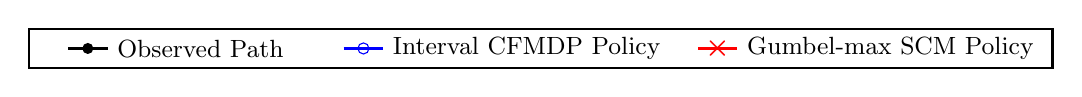
\begin{tikzpicture}[scale=1.0, every node/.style={scale=1.0}]
            \draw[thick, black] (-3, -0.25) rectangle (10, 0.25);
            %
            \draw[black, line width=1pt] (-2.5, 0.0) -- (-2,0.0);
            \fill[black] (-2.25,0.0) circle (2pt); %
            \node[right] at (-2,0.0) {\small Observed Path};
            
            %
            \draw[blue, line width=1pt] (1.0,0.0) -- (1.5,0.0);
            \node[draw=blue, circle, minimum size=4pt, inner sep=0pt] at (1.25,0.0) {}; %
            \node[right] at (1.5,0.0) {\small Interval CFMDP Policy};
            
            %
            \draw[red, line width=1pt] (5.5,0) -- (6,0);
            \node[red] at (5.75,0) {$\boldsymbol{\times}$}; %
            \node[right] at (6,0) {\small Gumbel-max SCM Policy};
        \end{tikzpicture}
    }\\
    %
    \subfigure[\footnotesize Lowest cumulative reward: Interval CFMDP ($312$), Gumbel-max SCM ($312$)]{%
        \resizebox{0.76\columnwidth}{!}{
             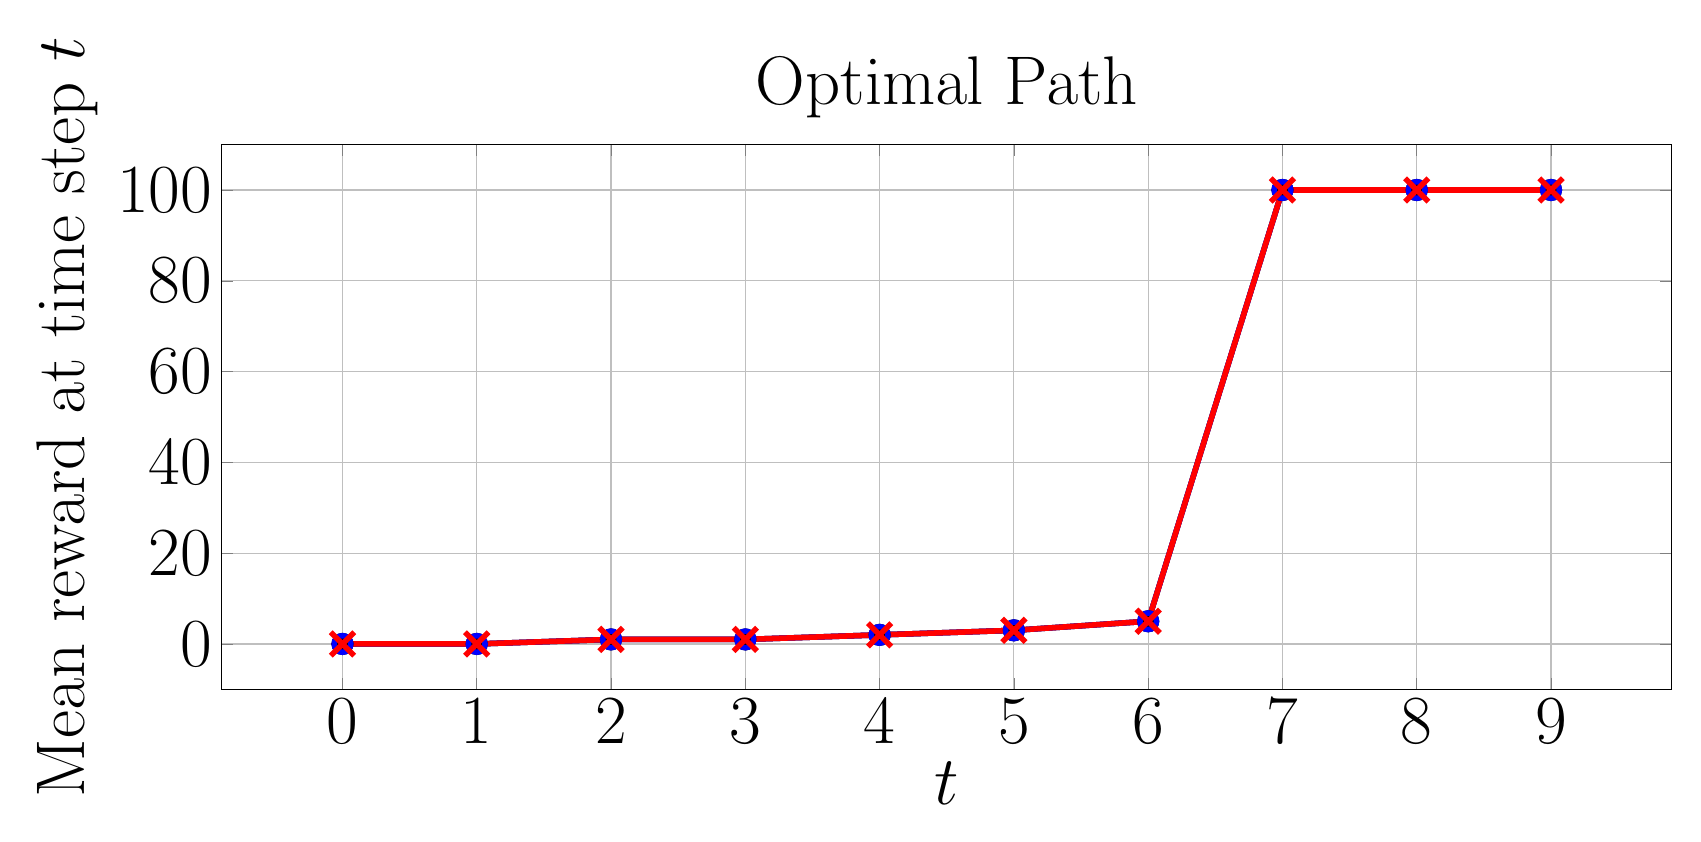
\begin{tikzpicture}
                \begin{axis}[
                    xlabel={$t$},
                    ylabel={Mean reward at time step $t$},
                    title={Optimal Path},
                    grid=both,
                    width=20cm, height=8.5cm,
                    every axis/.style={font=\Huge},
                    %
                ]
                \addplot[
                    color=black, %
                    mark=*, %
                    line width=2pt,
                    mark size=3pt,
                    error bars/.cd,
                    y dir=both, %
                    y explicit, %
                    error bar style={line width=1pt,solid},
                    error mark options={line width=1pt,mark size=4pt,rotate=90}
                ]
                coordinates {
                    (0, 0.0)  +- (0, 0.0)
                    (1, 0.0)  +- (0, 0.0) 
                    (2, 1.0)  +- (0, 0.0) 
                    (3, 1.0)  +- (0, 0.0)
                    (4, 2.0)  +- (0, 0.0)
                    (5, 3.0) +- (0, 0.0)
                    (6, 5.0) +- (0, 0.0)
                    (7, 100.0) +- (0, 0.0)
                    (8, 100.0) +- (0, 0.0)
                    (9, 100.0) +- (0, 0.0)
                };
                %
                \addplot[
                    color=blue, %
                    mark=o, %
                    line width=2pt,
                    mark size=3pt,
                    error bars/.cd,
                    y dir=both, %
                    y explicit, %
                    error bar style={line width=1pt,solid},
                    error mark options={line width=1pt,mark size=4pt,rotate=90}
                ]
                 coordinates {
                    (0, 0.0)  +- (0, 0.0)
                    (1, 0.0)  +- (0, 0.0) 
                    (2, 1.0)  +- (0, 0.0) 
                    (3, 1.0)  +- (0, 0.0)
                    (4, 2.0)  +- (0, 0.0)
                    (5, 3.0) +- (0, 0.0)
                    (6, 5.0) +- (0, 0.0)
                    (7, 100.0) +- (0, 0.0)
                    (8, 100.0) +- (0, 0.0)
                    (9, 100.0) +- (0, 0.0)
                };
                %
                \addplot[
                    color=red, %
                    mark=x, %
                    line width=2pt,
                    mark size=6pt,
                    error bars/.cd,
                    y dir=both, %
                    y explicit, %
                    error bar style={line width=1pt,solid},
                    error mark options={line width=1pt,mark size=4pt,rotate=90}
                ]
                coordinates {
                    (0, 0.0)  +- (0, 0.0)
                    (1, 0.0)  +- (0, 0.0) 
                    (2, 1.0)  +- (0, 0.0) 
                    (3, 1.0)  +- (0, 0.0)
                    (4, 2.0)  +- (0, 0.0)
                    (5, 3.0) +- (0, 0.0)
                    (6, 5.0) +- (0, 0.0)
                    (7, 100.0) +- (0, 0.0)
                    (8, 100.0) +- (0, 0.0)
                    (9, 100.0) +- (0, 0.0)
                };
                \end{axis}
            \end{tikzpicture}
         }
    }
    \hspace{1cm}
    \subfigure[\footnotesize Lowest cumulative reward: Interval CFMDP ($19$), Gumbel-max SCM ($-88$)]{%
         \resizebox{0.76\columnwidth}{!}{
            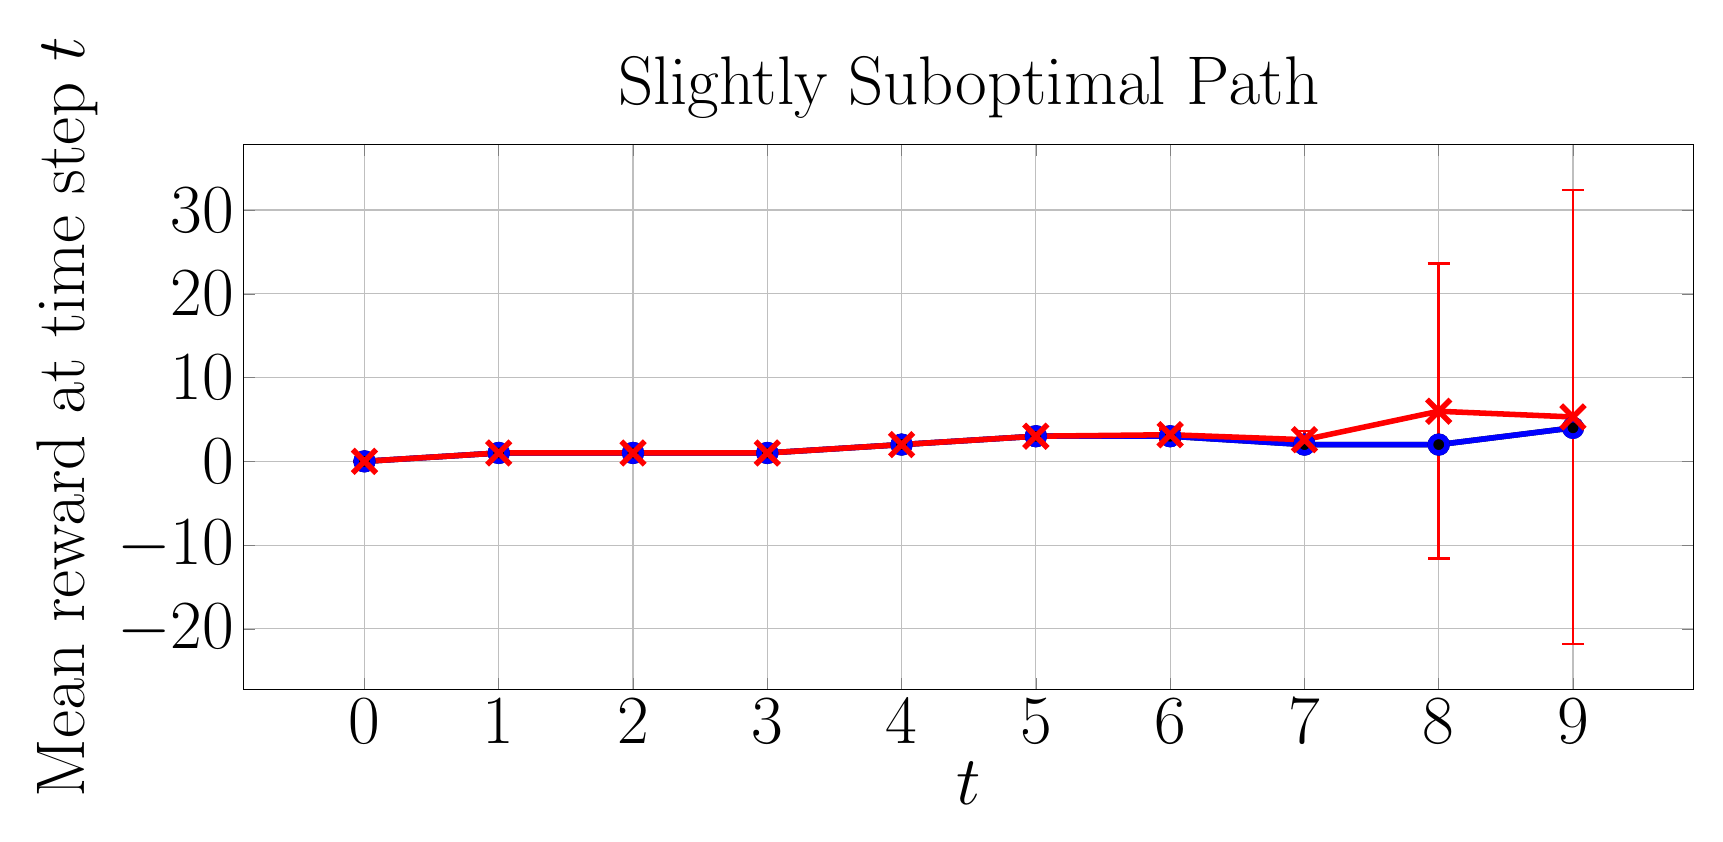
\begin{tikzpicture}
                \begin{axis}[
                    xlabel={$t$},
                    ylabel={Mean reward at time step $t$},
                    title={Slightly Suboptimal Path},
                    grid=both,
                    width=20cm, height=8.5cm,
                    every axis/.style={font=\Huge},
                    %
                ]
                \addplot[
                    color=black, %
                    mark=*, %
                    line width=2pt,
                    mark size=3pt,
                    error bars/.cd,
                    y dir=both, %
                    y explicit, %
                    error bar style={line width=1pt,solid},
                    error mark options={line width=1pt,mark size=4pt,rotate=90}
                ]
              coordinates {
                    (0, 0.0)  +- (0, 0.0)
                    (1, 1.0)  +- (0, 0.0) 
                    (2, 1.0)  +- (0, 0.0) 
                    (3, 1.0)  +- (0, 0.0)
                    (4, 2.0)  +- (0, 0.0)
                    (5, 3.0) +- (0, 0.0)
                    (6, 3.0) +- (0, 0.0)
                    (7, 2.0) +- (0, 0.0)
                    (8, 2.0) +- (0, 0.0)
                    (9, 4.0) +- (0, 0.0)
                };
                %
                \addplot[
                    color=blue, %
                    mark=o, %
                    line width=2pt,
                    mark size=3pt,
                    error bars/.cd,
                    y dir=both, %
                    y explicit, %
                    error bar style={line width=1pt,solid},
                    error mark options={line width=1pt,mark size=4pt,rotate=90}
                ]
              coordinates {
                    (0, 0.0)  +- (0, 0.0)
                    (1, 1.0)  +- (0, 0.0) 
                    (2, 1.0)  +- (0, 0.0) 
                    (3, 1.0)  +- (0, 0.0)
                    (4, 2.0)  +- (0, 0.0)
                    (5, 3.0) +- (0, 0.0)
                    (6, 3.0) +- (0, 0.0)
                    (7, 2.0) +- (0, 0.0)
                    (8, 2.0) +- (0, 0.0)
                    (9, 4.0) +- (0, 0.0)
                };
                %
                \addplot[
                    color=red, %
                    mark=x, %
                    line width=2pt,
                    mark size=6pt,
                    error bars/.cd,
                    y dir=both, %
                    y explicit, %
                    error bar style={line width=1pt,solid},
                    error mark options={line width=1pt,mark size=4pt,rotate=90}
                ]
                coordinates {
                    (0, 0.0)  +- (0, 0.0)
                    (1, 1.0)  +- (0, 0.0) 
                    (2, 1.0)  +- (0, 0.0) 
                    (3, 1.0)  +- (0, 0.0)
                    (4, 2.0)  += (0, 0.0)
                    (5, 3.0)  += (0, 0.0)
                    (6, 3.17847) += (0, 0.62606746) -= (0, 0.62606746)
                    (7, 2.5832885) += (0, 1.04598233) -= (0, 1.04598233)
                    (8, 5.978909) += (0, 17.60137623) -= (0, 17.60137623)
                    (9, 5.297059) += (0, 27.09227512) -= (0, 27.09227512)
                };
                \end{axis}
            \end{tikzpicture}
         }
    }\\[-1.5pt]
    \subfigure[\footnotesize Lowest cumulative reward: Interval CFMDP ($14$), Gumbel-max SCM ($-598$)]{%
         \resizebox{0.76\columnwidth}{!}{
             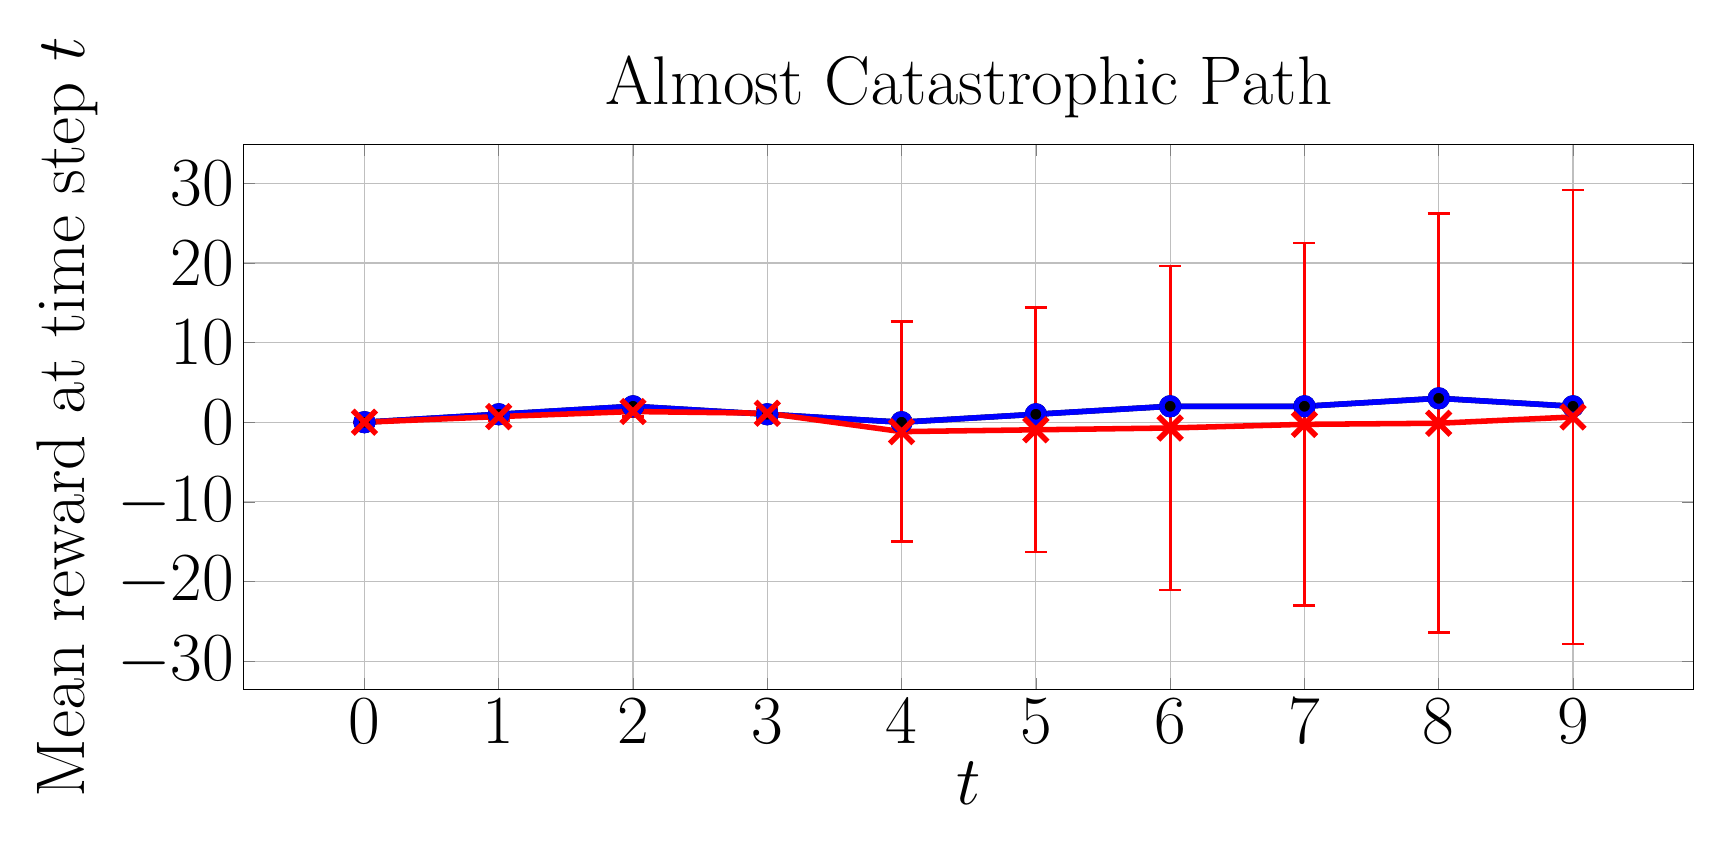
\begin{tikzpicture}
                \begin{axis}[
                    xlabel={$t$},
                    ylabel={Mean reward at time step $t$},
                    title={Almost Catastrophic Path},
                    grid=both,
                    width=20cm, height=8.5cm,
                    every axis/.style={font=\Huge},
                    %
                ]
                \addplot[
                    color=black, %
                    mark=*, %
                    line width=2pt,
                    mark size=3pt,
                    error bars/.cd,
                    y dir=both, %
                    y explicit, %
                    error bar style={line width=1pt,solid},
                    error mark options={line width=1pt,mark size=4pt,rotate=90}
                ]
                coordinates {
                    (0, 0.0)  +- (0, 0.0)
                    (1, 1.0)  +- (0, 0.0) 
                    (2, 2.0)  +- (0, 0.0) 
                    (3, 1.0)  +- (0, 0.0)
                    (4, 0.0)  +- (0, 0.0)
                    (5, 1.0) +- (0, 0.0)
                    (6, 2.0) +- (0, 0.0)
                    (7, 2.0) +- (0, 0.0)
                    (8, 3.0) +- (0, 0.0)
                    (9, 2.0) +- (0, 0.0)
                };
                %
                \addplot[
                    color=blue, %
                    mark=o, %
                    line width=2pt,
                    mark size=3pt,
                    error bars/.cd,
                    y dir=both, %
                    y explicit, %
                    error bar style={line width=1pt,solid},
                    error mark options={line width=1pt,mark size=4pt,rotate=90}
                ]
                coordinates {
                    (0, 0.0)  +- (0, 0.0)
                    (1, 1.0)  +- (0, 0.0) 
                    (2, 2.0)  +- (0, 0.0) 
                    (3, 1.0)  +- (0, 0.0)
                    (4, 0.0)  +- (0, 0.0)
                    (5, 1.0) +- (0, 0.0)
                    (6, 2.0) +- (0, 0.0)
                    (7, 2.0) +- (0, 0.0)
                    (8, 3.0) +- (0, 0.0)
                    (9, 2.0) +- (0, 0.0)
                };
                %
                \addplot[
                    color=red, %
                    mark=x, %
                    line width=2pt,
                    mark size=6pt,
                    error bars/.cd,
                    y dir=both, %
                    y explicit, %
                    error bar style={line width=1pt,solid},
                    error mark options={line width=1pt,mark size=4pt,rotate=90}
                ]
                coordinates {
                    (0, 0.0)  +- (0, 0.0)
                    (1, 0.7065655)  +- (0, 0.4553358) 
                    (2, 1.341673)  +- (0, 0.67091621) 
                    (3, 1.122926)  +- (0, 0.61281824)
                    (4, -1.1821935)  +- (0, 13.82444042)
                    (5, -0.952399)  +- (0, 15.35195457)
                    (6, -0.72672) +- (0, 20.33508414)
                    (7, -0.268983) +- (0, 22.77861454)
                    (8, -0.1310835) +- (0, 26.31013314)
                    (9, 0.65806) +- (0, 28.50670214)
                };
                %
            %
            %
            %
            %
            %
            %
            %
            %
            %
            %
            %
            %
            %
            %
            %
            %
            %
            %
                \end{axis}
            \end{tikzpicture}
         }
    }
    \hspace{1cm}
    \subfigure[\footnotesize Lowest cumulative reward: Interval CFMDP ($-698$), Gumbel-max SCM ($-698$)]{%
         \resizebox{0.76\columnwidth}{!}{
            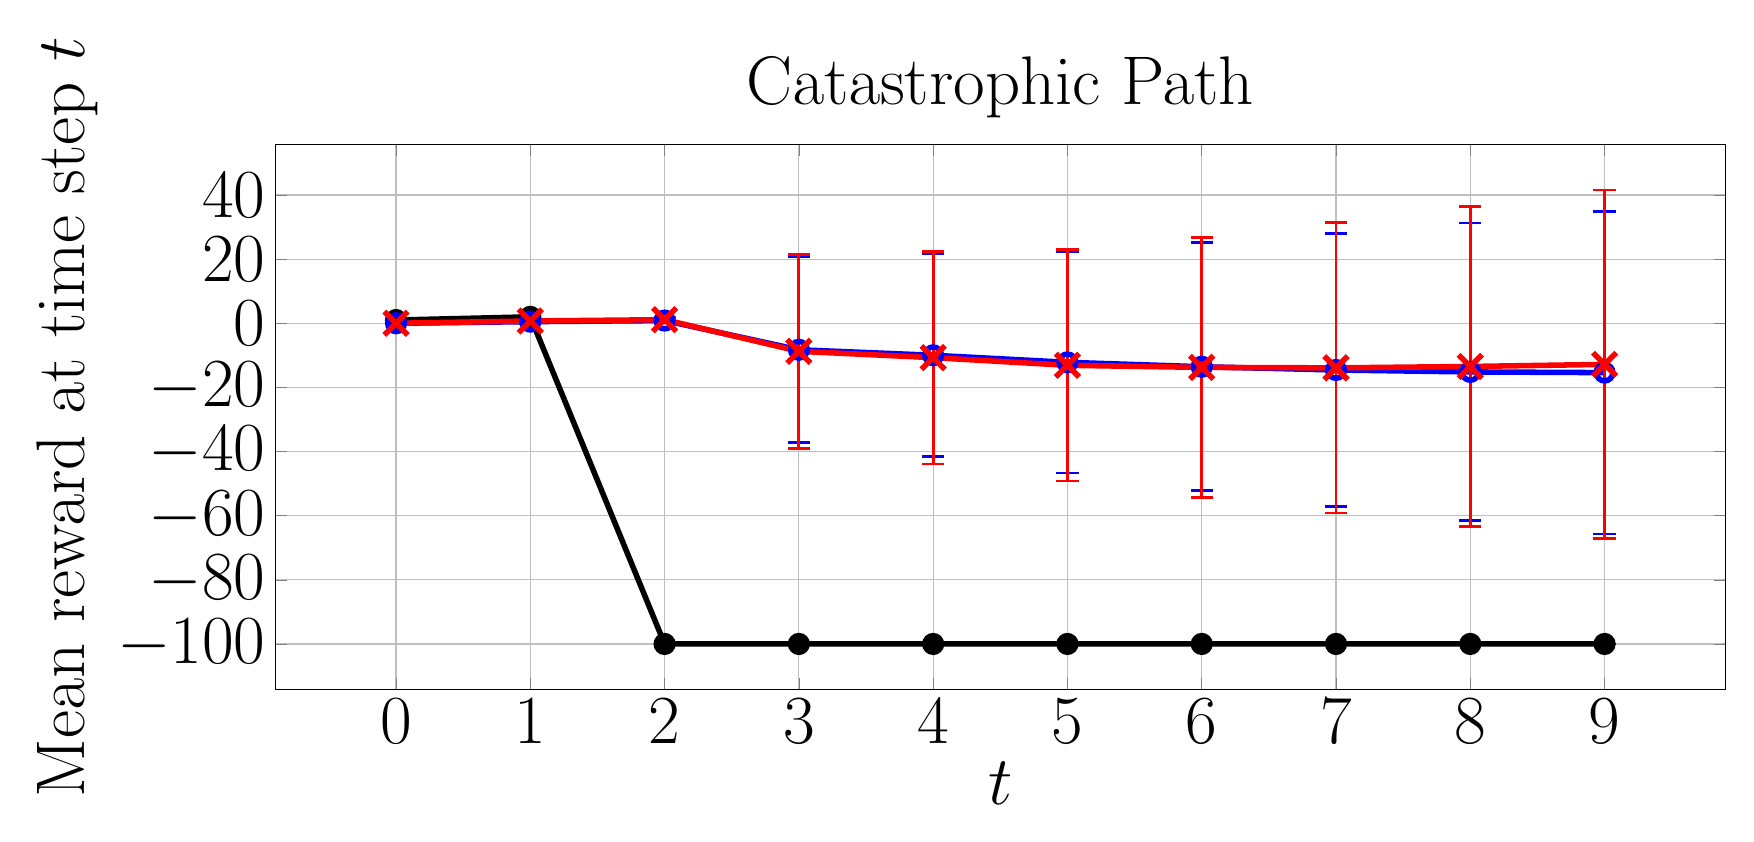
\begin{tikzpicture}
                \begin{axis}[
                    xlabel={$t$},
                    ylabel={Mean reward at time step $t$},
                    title={Catastrophic Path},
                    grid=both,
                    width=20cm, height=8.5cm,
                    every axis/.style={font=\Huge},
                    %
                ]
                \addplot[
                    color=black, %
                    mark=*, %
                    line width=2pt,
                    mark size=3pt,
                    error bars/.cd,
                    y dir=both, %
                    y explicit, %
                    error bar style={line width=1pt,solid},
                    error mark options={line width=1pt,mark size=4pt,rotate=90}
                ]
                coordinates {
                    (0, 1.0)  +- (0, 0.0)
                    (1, 2.0)  +- (0, 0.0) 
                    (2, -100.0)  +- (0, 0.0) 
                    (3, -100.0)  +- (0, 0.0)
                    (4, -100.0)  +- (0, 0.0)
                    (5, -100.0) +- (0, 0.0)
                    (6, -100.0) +- (0, 0.0)
                    (7, -100.0) +- (0, 0.0)
                    (8, -100.0) +- (0, 0.0)
                    (9, -100.0) +- (0, 0.0)
                };
                %
                \addplot[
                    color=blue, %
                    mark=o, %
                    line width=2pt,
                    mark size=3pt,
                    error bars/.cd,
                    y dir=both, %
                    y explicit, %
                    error bar style={line width=1pt,solid},
                    error mark options={line width=1pt,mark size=4pt,rotate=90}
                ]
                coordinates {
                    (0, 0.0)  +- (0, 0.0)
                    (1, 0.504814)  +- (0, 0.49997682) 
                    (2, 0.8439835)  +- (0, 0.76831917) 
                    (3, -8.2709165)  +- (0, 28.93656754)
                    (4, -9.981082)  +- (0, 31.66825363)
                    (5, -12.1776325) +- (0, 34.53463233)
                    (6, -13.556076) +- (0, 38.62845372)
                    (7, -14.574418) +- (0, 42.49603359)
                    (8, -15.1757075) +- (0, 46.41913968)
                    (9, -15.3900395) +- (0, 50.33563368)
                };
                %
                \addplot[
                    color=red, %
                    mark=x, %
                    line width=2pt,
                    mark size=6pt,
                    error bars/.cd,
                    y dir=both, %
                    y explicit, %
                    error bar style={line width=1pt,solid},
                    error mark options={line width=1pt,mark size=4pt,rotate=90}
                ]
                coordinates {
                    (0, 0.0)  +- (0, 0.0)
                    (1, 0.701873)  +- (0, 0.45743556) 
                    (2, 1.1227805)  +- (0, 0.73433129) 
                    (3, -8.7503255)  +- (0, 30.30257976)
                    (4, -10.722092)  +- (0, 33.17618589)
                    (5, -13.10721)  +- (0, 36.0648089)
                    (6, -13.7631645) +- (0, 40.56553451)
                    (7, -13.909043) +- (0, 45.23829402)
                    (8, -13.472517) +- (0, 49.96270296)
                    (9, -12.8278835) +- (0, 54.38618735)
                };
                %
            %
            %
            %
            %
            %
            %
            %
            %
            %
            %
            %
            %
            %
            %
            %
            %
            %
            %
                \end{axis}
            \end{tikzpicture}
         }
    }
    \caption{Average instant reward of CF paths induced by policies on GridWorld $p=0.4$.}
    \label{fig: reward p=0.4}
\end{figure*}

\subsection{Experimental Setup}
To compare policy performance, we measure the average rewards of counterfactual paths induced by our policy and the Gumbel-max policy by uniformly sampling $200$ counterfactual MDPs from the ICFMDP and generating $10,000$ counterfactual paths over each sampled CFMDP. \jl{Since the interval CFMDP depends on the observed path, we select $4$  paths of varying optimality to evaluate how the observed path impacts the performance of both policies: an optimal path, a slightly suboptimal path that could reach the optimal reward with a few changes, a catastrophic path that enters a catastrophic, terminal state with low reward, and an almost catastrophic path that was close to entering a catastrophic state.} When measuring the average probability bound widths and execution time needed to generate the ICFMDPs, we averaged over $20$ randomly generated observed paths
\footnote{Further training details are provided in Appendix \ref{app: training details}, and the code is provided at \href{https://github.com/ddv-lab/robust-cf-inference-in-MDPs}{https://github.com/ddv-lab/robust-cf-inference-in-MDPs}
%
%
.}.

\subsection{GridWorld}
\jl{The GridWorld MDP is a $4 \times 4$ grid where an agent must navigate from the top-left corner to the goal state in the bottom-right corner, avoiding a dangerous terminal state in the centre. At each time step, the agent can move up, down, left, or right, but there is a small probability (controlled by hyper-parameter $p$) of moving in an unintended direction. As the agent nears the goal, the reward for each state increases, culminating in a reward of $+100$ for reaching the goal. Entering the dangerous state results in a penalty of $-100$. We use two versions of GridWorld: a less stochastic version with $p=0.9$ (i.e., $90$\% chance of moving in the chosen direction) and a more stochastic version with $p=0.4$.}

\paragraph{GridWorld ($p=0.9$)}
When $p=0.9$, the counterfactual probability bounds are typically narrow (see Table \ref{tab:nonzero_probs} for average measurements). Consequently, as shown in Figure \ref{fig: reward p=0.9}, both policies are nearly identical and perform similarly well across the optimal, slightly suboptimal, and catastrophic paths.
%
However, for the almost catastrophic path, the interval CFMDP path is more conservative and follows the observed path more closely (as this is where the probability bounds are narrowest), which typically requires one additional step to reach the goal state than the Gumbel-max SCM policy.
%

\paragraph{GridWorld ($p=0.4$)}
\jl{When $p=0.4$, the GridWorld environment becomes more uncertain, increasing the risk of entering the dangerous state even if correct actions are chosen. Thus, as shown in Figure \ref{fig: reward p=0.4}, the interval CFMDP policy adopts a more conservative approach, avoiding deviation from the observed policy if it cannot guarantee higher counterfactual rewards (see the slightly suboptimal and almost catastrophic paths), whereas the Gumbel-max SCM is inconsistent: it can yield higher rewards, but also much lower rewards, reflected in the wide error bars.} For the catastrophic path, both policies must deviate from the observed path to achieve a higher reward and, in this case, perform similarly.
%
%
%
%
\subsection{Sepsis}
The Sepsis MDP \citep{oberst2019counterfactual} simulates trajectories of Sepsis patients. Each state consists of four vital signs (heart rate, blood pressure, oxygen concentration, and glucose levels), categorised as low, normal, or high.
and three treatments that can be toggled on/off at each time step (8 actions in total). Unlike \citet{oberst2019counterfactual}, we scale rewards based on the number of out-of-range vital signs, between $-1000$ (patient dies) and $1000$ (patient discharged). \jl{Like the GridWorld $p=0.4$ experiment, the Sepsis MDP is highly uncertain, as many states are equally likely to lead to optimal and poor outcomes. Thus, as shown in Figure \ref{fig: reward sepsis}, both policies follow the observed optimal and almost catastrophic paths to guarantee rewards are no worse than the observation.} However, improving the catastrophic path requires deviating from the observation. Here, the Gumbel-max SCM policy, on average, performs better than the interval CFMDP policy. But, since both policies have lower bounds clipped at $-1000$, neither policy reliably improves over the observation. In contrast, for the slightly suboptimal path, the interval CFMDP policy performs significantly better, shown by its higher lower bounds. 
Moreover, in these two cases, the worst-case counterfactual path generated by the interval CFMDP policy is better than that of the Gumbel-max SCM policy,
indicating its greater robustness.
%
\begin{figure*}
    \centering
     \resizebox{0.6\textwidth}{!}{
        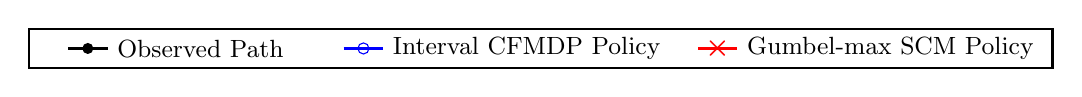
\begin{tikzpicture}[scale=1.0, every node/.style={scale=1.0}]
            \draw[thick, black] (-3, -0.25) rectangle (10, 0.25);
            %
            \draw[black, line width=1pt] (-2.5, 0.0) -- (-2,0.0);
            \fill[black] (-2.25,0.0) circle (2pt); %
            \node[right] at (-2,0.0) {\small Observed Path};
            
            %
            \draw[blue, line width=1pt] (1.0,0.0) -- (1.5,0.0);
            \node[draw=blue, circle, minimum size=4pt, inner sep=0pt] at (1.25,0.0) {}; %
            \node[right] at (1.5,0.0) {\small Interval CFMDP Policy};
            
            %
            \draw[red, line width=1pt] (5.5,0) -- (6,0);
            \node[red] at (5.75,0) {$\boldsymbol{\times}$}; %
            \node[right] at (6,0) {\small Gumbel-max SCM Policy};
        \end{tikzpicture}
    }\\
    \subfigure[\footnotesize Lowest cumulative reward: Interval CFMDP ($8000$), Gumbel-max SCM ($8000$)]{%
         \resizebox{0.76\columnwidth}{!}{
             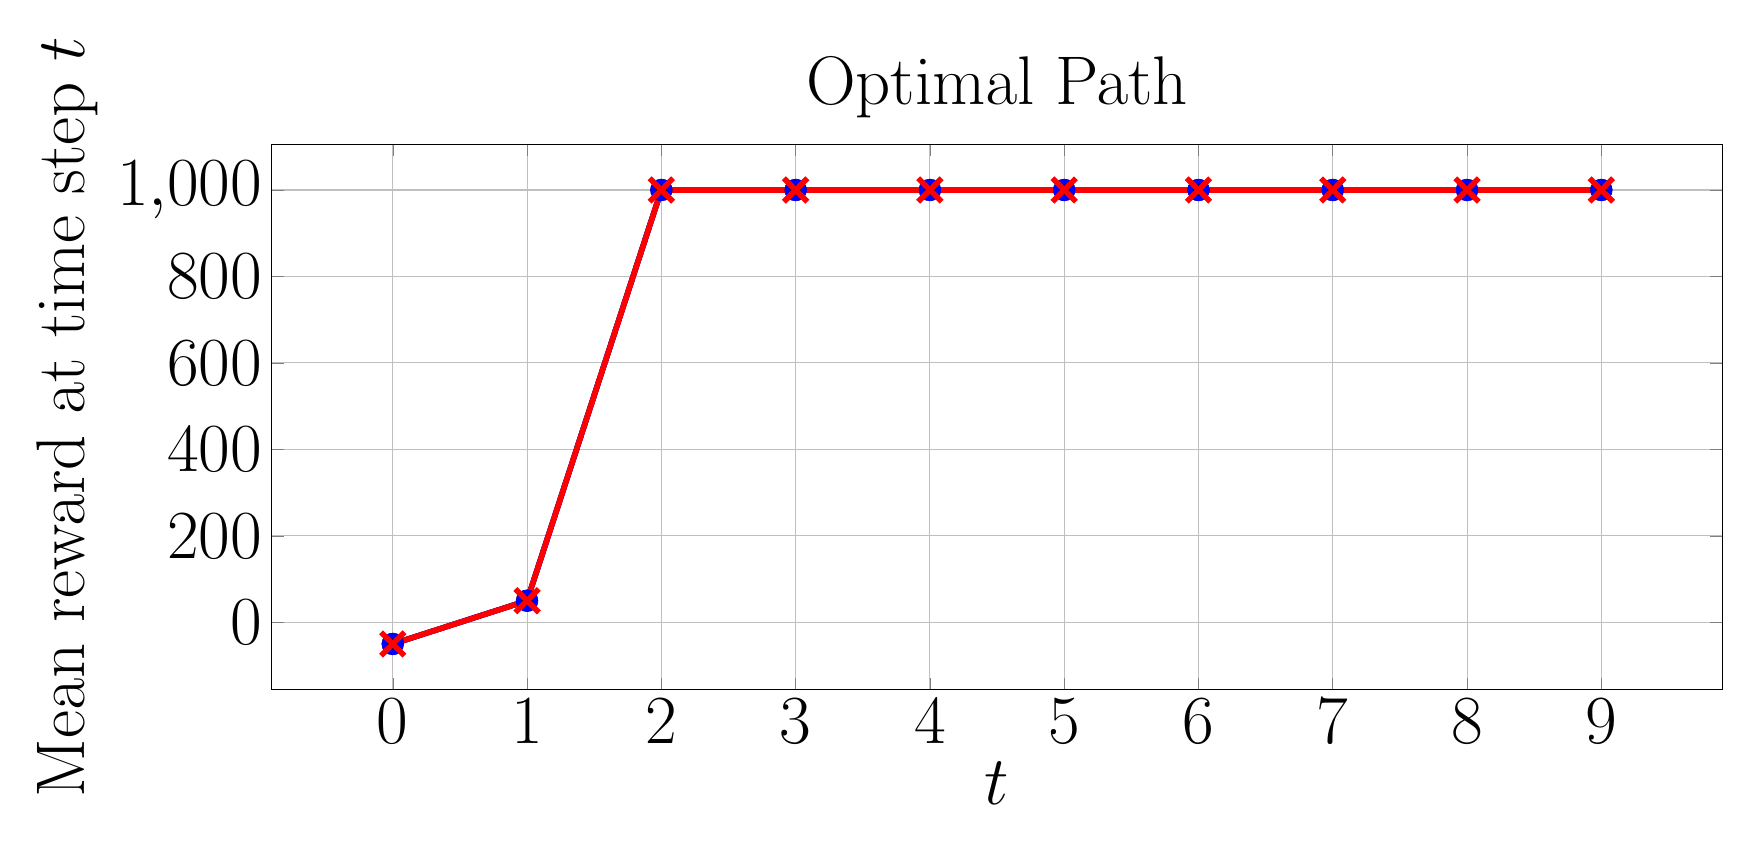
\begin{tikzpicture}
                \begin{axis}[
                    xlabel={$t$},
                    ylabel={Mean reward at time step $t$},
                    title={Optimal Path},
                    grid=both,
                    width=20cm, height=8.5cm,
                    every axis/.style={font=\Huge},
                    %
                ]
                \addplot[
                    color=black, %
                    mark=*, %
                    line width=2pt,
                    mark size=3pt,
                ]
                coordinates {
                    (0, -50.0)
                    (1, 50.0)
                    (2, 1000.0)
                    (3, 1000.0)
                    (4, 1000.0)
                    (5, 1000.0)
                    (6, 1000.0)
                    (7, 1000.0)
                    (8, 1000.0)
                    (9, 1000.0)
                };
                %
                \addplot[
                    color=blue, %
                    mark=o, %
                    line width=2pt,
                    mark size=3pt,
                    error bars/.cd,
                    y dir=both, %
                    y explicit, %
                    error bar style={line width=1pt,solid},
                    error mark options={line width=1pt,mark size=4pt,rotate=90}
                ]
                coordinates {
                    (0, -50.0)  +- (0, 0.0)
                    (1, 50.0)  +- (0, 0.0) 
                    (2, 1000.0)  +- (0, 0.0) 
                    (3, 1000.0)  +- (0, 0.0)
                    (4, 1000.0)  +- (0, 0.0)
                    (5, 1000.0) +- (0, 0.0)
                    (6, 1000.0) +- (0, 0.0)
                    (7, 1000.0) +- (0, 0.0)
                    (8, 1000.0) +- (0, 0.0)
                    (9, 1000.0) +- (0, 0.0)
                };
                %
                \addplot[
                    color=red, %
                    mark=x, %
                    line width=2pt,
                    mark size=6pt,
                    error bars/.cd,
                    y dir=both, %
                    y explicit, %
                    error bar style={line width=1pt,solid},
                    error mark options={line width=1pt,mark size=4pt,rotate=90}
                ]
                coordinates {
                    (0, -50.0)  +- (0, 0.0)
                    (1, 50.0)  +- (0, 0.0) 
                    (2, 1000.0)  +- (0, 0.0) 
                    (3, 1000.0)  +- (0, 0.0)
                    (4, 1000.0)  +- (0, 0.0)
                    (5, 1000.0) +- (0, 0.0)
                    (6, 1000.0) +- (0, 0.0)
                    (7, 1000.0) +- (0, 0.0)
                    (8, 1000.0) +- (0, 0.0)
                    (9, 1000.0) +- (0, 0.0)
                };
                %
                \end{axis}
            \end{tikzpicture}
         }
    }
    \hspace{1cm}
    \subfigure[\footnotesize Lowest cumulative reward: Interval CFMDP ($-5980$), Gumbel-max SCM ($-8000$)]{%
         \resizebox{0.76\columnwidth}{!}{
            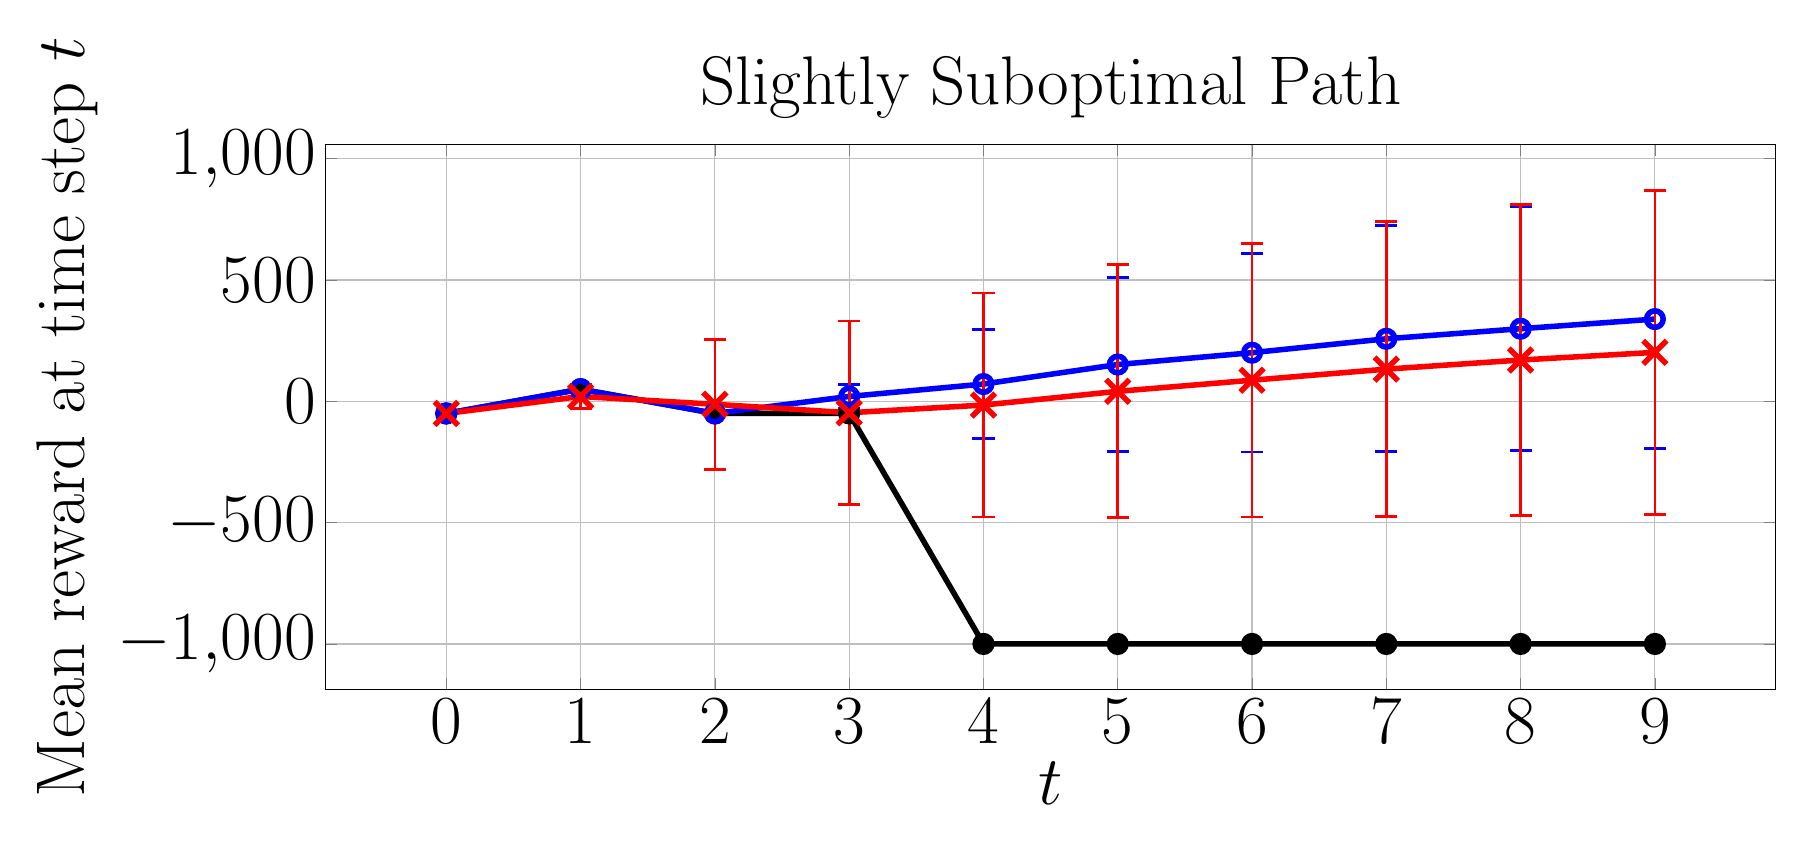
\begin{tikzpicture}
                \begin{axis}[
                    xlabel={$t$},
                    ylabel={Mean reward at time step $t$},
                    title={Slightly Suboptimal Path},
                    grid=both,
                    width=20cm, height=8.5cm,
                    every axis/.style={font=\Huge},
                    %
                ]
               \addplot[
                    color=black, %
                    mark=*, %
                    line width=2pt,
                    mark size=3pt,
                ]
                coordinates {
                    (0, -50.0)
                    (1, 50.0)
                    (2, -50.0)
                    (3, -50.0)
                    (4, -1000.0)
                    (5, -1000.0)
                    (6, -1000.0)
                    (7, -1000.0)
                    (8, -1000.0)
                    (9, -1000.0)
                };
                %
                \addplot[
                    color=blue, %
                    mark=o, %
                    line width=2pt,
                    mark size=3pt,
                    error bars/.cd,
                    y dir=both, %
                    y explicit, %
                    error bar style={line width=1pt,solid},
                    error mark options={line width=1pt,mark size=4pt,rotate=90}
                ]
                coordinates {
                    (0, -50.0)  +- (0, 0.0)
                    (1, 50.0)  +- (0, 0.0) 
                    (2, -50.0)  +- (0, 0.0) 
                    (3, 20.0631)  +- (0, 49.97539413)
                    (4, 71.206585)  +- (0, 226.02033693)
                    (5, 151.60797) +- (0, 359.23292559)
                    (6, 200.40593) +- (0, 408.86185176)
                    (7, 257.77948) +- (0, 466.10372804)
                    (8, 299.237465) +- (0, 501.82579506)
                    (9, 338.9129) +- (0, 532.06124996)
                };
                %
                \addplot[
                    color=red, %
                    mark=x, %
                    line width=2pt,
                    mark size=6pt,
                    error bars/.cd,
                    y dir=both, %
                    y explicit, %
                    error bar style={line width=1pt,solid},
                    error mark options={line width=1pt,mark size=4pt,rotate=90}
                ]
                coordinates {
                    (0, -50.0)  +- (0, 0.0)
                    (1, 20.00736)  +- (0, 49.99786741) 
                    (2, -12.282865)  +- (0, 267.598755) 
                    (3, -47.125995)  +- (0, 378.41755832)
                    (4, -15.381965)  +- (0, 461.77616558)
                    (5, 41.15459) +- (0, 521.53189262)
                    (6, 87.01595) +- (0, 564.22243126 )
                    (7, 132.62376) +- (0, 607.31338037)
                    (8, 170.168145) +- (0, 641.48013693)
                    (9, 201.813135) +- (0, 667.29441777)
                };
                %
                %
                %
                %
                %
                %
                %
                %
                %
                %
                %
                %
                %
                %
                %
                %
                %
                %
                %
                \end{axis}
            \end{tikzpicture}
         }
    }\\[-1.5pt]
    \subfigure[\footnotesize Lowest cumulative reward: Interval CFMDP ($100$), Gumbel-max SCM ($100$)]{%
         \resizebox{0.76\columnwidth}{!}{
             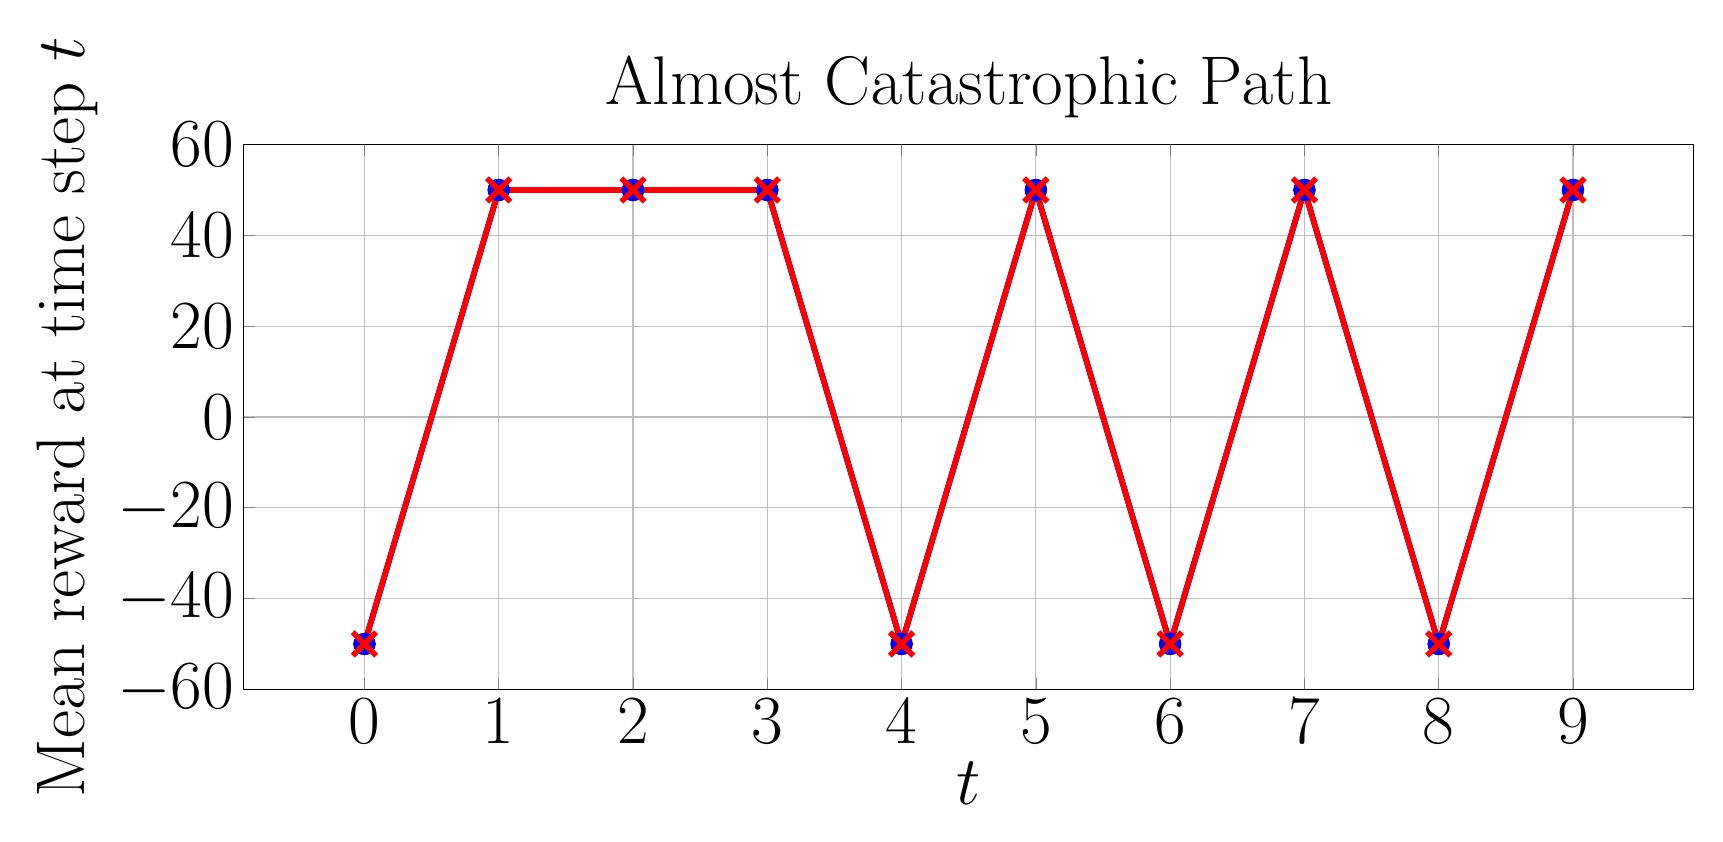
\begin{tikzpicture}
                \begin{axis}[
                    xlabel={$t$},
                    ylabel={Mean reward at time step $t$},
                    title={Almost Catastrophic Path},
                    grid=both,
                    every axis/.style={font=\Huge},
                    width=20cm, height=8.5cm,
                    %
                ]
               \addplot[
                    color=black, %
                    mark=*, %
                    line width=2pt,
                    mark size=3pt,
                ]
                coordinates {
                    (0, -50.0)
                    (1, 50.0)
                    (2, 50.0)
                    (3, 50.0)
                    (4, -50.0)
                    (5, 50.0)
                    (6, -50.0)
                    (7, 50.0)
                    (8, -50.0)
                    (9, 50.0)
                };
                %
                %
                \addplot[
                    color=blue, %
                    mark=o, %
                    line width=2pt,
                    mark size=3pt,
                    error bars/.cd,
                    y dir=both, %
                    y explicit, %
                    error bar style={line width=1pt,solid},
                    error mark options={line width=1pt,mark size=4pt,rotate=90}
                ]
                coordinates {
                    (0, -50.0)  +- (0, 0.0)
                    (1, 50.0)  +- (0, 0.0) 
                    (2, 50.0)  +- (0, 0.0) 
                    (3, 50.0)  +- (0, 0.0)
                    (4, -50.0)  +- (0, 0.0)
                    (5, 50.0) +- (0, 0.0)
                    (6, -50.0) +- (0, 0.0)
                    (7, 50.0) +- (0, 0.0)
                    (8, -50.0) +- (0, 0.0)
                    (9, 50.0) +- (0, 0.0)
                };
                %
                \addplot[
                    color=red, %
                    mark=x, %
                    line width=2pt,
                    mark size=6pt,
                    error bars/.cd,
                    y dir=both, %
                    y explicit, %
                    error bar style={line width=1pt,solid},
                    error mark options={line width=1pt,mark size=4pt,rotate=90}
                ]
                coordinates {
                    (0, -50.0)  +- (0, 0.0)
                    (1, 50.0)  +- (0, 0.0) 
                    (2, 50.0)  +- (0, 0.0) 
                    (3, 50.0)  +- (0, 0.0)
                    (4, -50.0)  +- (0, 0.0)
                    (5, 50.0) +- (0, 0.0)
                    (6, -50.0) +- (0, 0.0)
                    (7, 50.0) +- (0, 0.0)
                    (8, -50.0) +- (0, 0.0)
                    (9, 50.0) +- (0, 0.0)
                };
                %
                %
                %
                %
                %
                %
                %
                %
                %
                %
                %
                %
                %
                %
                %
                %
                %
                %
                %
                \end{axis}
            \end{tikzpicture}
         }
    }
    \hspace{1cm}
    \subfigure[\footnotesize Lowest cumulative reward: Interval CFMDP ($-7150$), Gumbel-max SCM ($-9050$)]{%
         \resizebox{0.76\columnwidth}{!}{
            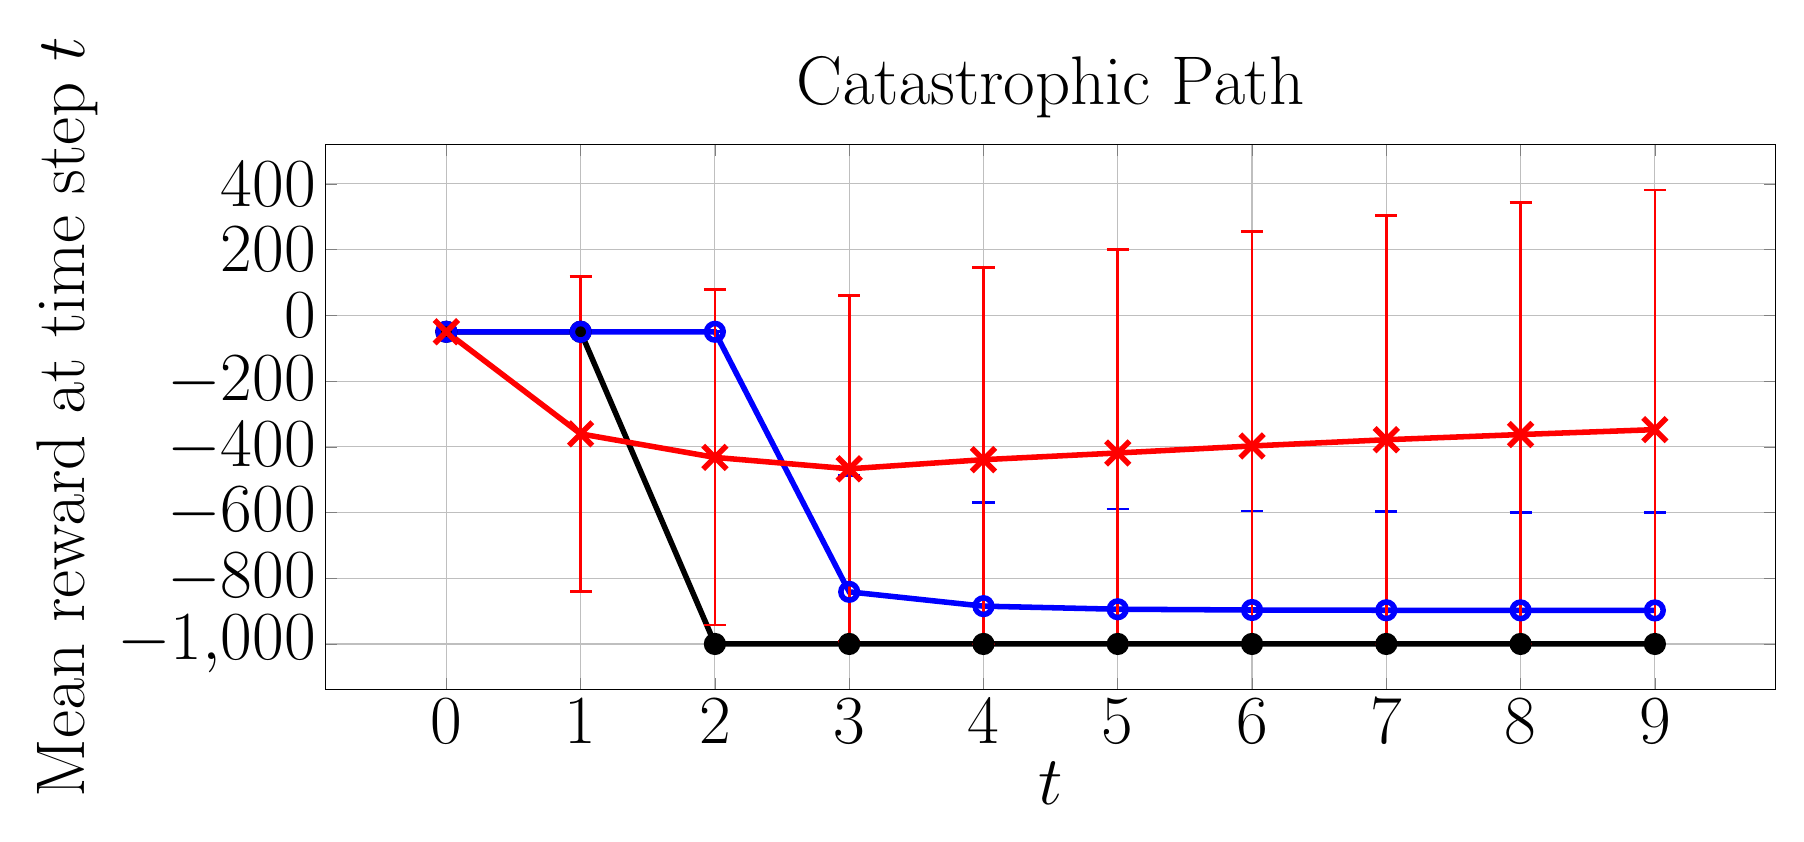
\begin{tikzpicture}
                \begin{axis}[
                    xlabel={$t$},
                    ylabel={Mean reward at time step $t$},
                    title={Catastrophic Path},
                    grid=both,
                    width=20cm, height=8.5cm,
                    every axis/.style={font=\Huge},
                    %
                ]
               \addplot[
                    color=black, %
                    mark=*, %
                    line width=2pt,
                    mark size=3pt,
                ]
                coordinates {
                    (0, -50.0)
                    (1, -50.0)
                    (2, -1000.0)
                    (3, -1000.0)
                    (4, -1000.0)
                    (5, -1000.0)
                    (6, -1000.0)
                    (7, -1000.0)
                    (8, -1000.0)
                    (9, -1000.0)
                };
                %
                %
                \addplot[
                    color=blue, %
                    mark=o, %
                    line width=2pt,
                    mark size=3pt,
                    error bars/.cd,
                    y dir=both, %
                    y explicit, %
                    error bar style={line width=1pt,solid},
                    error mark options={line width=1pt,mark size=4pt,rotate=90}
                ]
                coordinates {
                    (0, -50.0)  +- (0, 0.0)
                    (1, -50.0)  +- (0, 0.0) 
                    (2, -50.0)  +- (0, 0.0) 
                    (3, -841.440725)  += (0, 354.24605512) -= (0, 158.559275)
                    (4, -884.98225)  += (0, 315.37519669) -= (0, 115.01775)
                    (5, -894.330425) += (0, 304.88572805) -= (0, 105.669575)
                    (6, -896.696175) += (0, 301.19954514) -= (0, 103.303825)
                    (7, -897.4635) += (0, 299.61791279) -= (0, 102.5365)
                    (8, -897.77595) += (0, 298.80392585) -= (0, 102.22405)
                    (9, -897.942975) += (0, 298.32920557) -= (0, 102.057025)
                };
                %
                \addplot[
                    color=red, %
                    mark=x, %
                    line width=2pt,
                    mark size=6pt,
                    error bars/.cd,
                    y dir=both, %
                    y explicit, %
                    error bar style={line width=1pt,solid},
                    error mark options={line width=1pt,mark size=4pt,rotate=90}
                ]
            coordinates {
                    (0, -50.0)  +- (0, 0.0)
                    (1, -360.675265)  +- (0, 479.39812699) 
                    (2, -432.27629)  +- (0, 510.38620897) 
                    (3, -467.029545)  += (0, 526.36009628) -= (0, 526.36009628)
                    (4, -439.17429)  += (0, 583.96638919) -= (0, 560.82571)
                    (5, -418.82704) += (0, 618.43027478) -= (0, 581.17296)
                    (6, -397.464895) += (0, 652.67322574) -= (0, 602.535105)
                    (7, -378.49052) += (0, 682.85407033) -= (0, 621.50948)
                    (8, -362.654195) += (0, 707.01412023) -= (0, 637.345805)
                    (9, -347.737935) += (0, 729.29076479) -= (0, 652.262065)
                };
                %
                %
                %
                %
                %
                %
                %
                %
                %
                %
                %
                %
                %
                %
                %
                %
                %
                %
                %
                \end{axis}
            \end{tikzpicture}
         }
    }
    \caption{Average instant reward of CF paths induced by policies on Sepsis.}
    \label{fig: reward sepsis}
\end{figure*}

%
%
%
\subsection{Interval CFMDP Bounds}
%
%
Table \ref{tab:nonzero_probs} presents the mean counterfactual probability bound widths (excluding transitions where the upper bound is $0$) for each MDP, averaged over 20 observed paths. We compare the bounds under counterfactual stability (CS) and monotonicity (M) assumptions, CS alone, and no assumptions. This shows that the assumptions marginally reduce the bound widths, indicating the assumptions tighten the bounds without excluding too many causal models, as intended.
\renewcommand{\arraystretch}{1}

\begin{table}
\centering
\caption{Mean width of counterfactual probability bounds}
\resizebox{0.8\columnwidth}{!}{%
\begin{tabular}{|c|c|c|c|}
\hline
\multirow{2}{*}{\textbf{Environment}} & \multicolumn{3}{c|}{\textbf{Assumptions}} \\ \cline{2-4}
 & \textbf{CS + M} & \textbf{CS} & \textbf{None\tablefootnote{\jl{Equivalent to \citet{li2024probabilities}'s bounds (see Section \ref{sec: equivalence with Li}).}}} \\ \hline
\textbf{GridWorld} ($p=0.9$) & 0.0817 & 0.0977 & 0.100 \\ \hline
\textbf{GridWorld} ($p=0.4$) & 0.552  & 0.638  & 0.646 \\ \hline
\textbf{Sepsis} & 0.138 & 0.140 & 0.140 \\ \hline
\end{tabular}
}
\label{tab:nonzero_probs}
\end{table}


\subsection{Execution Times}
Table \ref{tab: times} compares the average time needed to generate the interval CFMDP vs.\ the Gumbel-max SCM CFMDP for 20 observations.
The GridWorld algorithms were run single-threaded, while the Sepsis experiments were run in parallel.
Generating the interval CFMDP is significantly faster as it uses exact analytical bounds, whereas the Gumbel-max CFMDP requires sampling from the Gumbel distribution to estimate counterfactual transition probabilities. \jl{Since constructing the counterfactual MDP models is the main bottleneck in both approaches, ours is more efficient overall and suitable for larger MDPs.}
\begin{table}
\centering
\caption{Mean execution time to generate CFMDPs}
\resizebox{0.99\columnwidth}{!}{%
\begin{tabular}{|c|c|c|}
\hline
\multirow{2}{*}{\textbf{Environment}} & \multicolumn{2}{c|}{\textbf{Mean Execution Time (s)}} \\ \cline{2-3} 
                                      & \textbf{Interval CFMDP} & \textbf{Gumbel-max CFMDP} \\ \hline
\textbf{GridWorld ($p=0.9$) }                  & 0.261                   & 56.1                      \\ \hline
\textbf{GridWorld ($p=0.4$)  }                 & 0.336                   & 54.5                      \\ \hline
\textbf{Sepsis}                                 & 688                     & 2940                      \\ \hline
\end{tabular}%
}
\label{tab: times}
\end{table}

\section{Conclusion}
In this work, we propose a simple yet effective approach, called SMILE, for graph few-shot learning with fewer tasks. Specifically, we introduce a novel dual-level mixup strategy, including within-task and across-task mixup, for enriching the diversity of nodes within each task and the diversity of tasks. Also, we incorporate the degree-based prior information to learn expressive node embeddings. Theoretically, we prove that SMILE effectively enhances the model's generalization performance. Empirically, we conduct extensive experiments on multiple benchmarks and the results suggest that SMILE significantly outperforms other baselines, including both in-domain and cross-domain few-shot settings.
% \IEEEtriggeratref{16}
\bibliographystyle{IEEEtran}
\bibliography{cite}

\end{document}
